\documentclass[10pt,a4paper]{article}
\newcommand{\runningtitle}{Neural topic scores in diabetic foot ulcer research}
\usepackage[margin=15mm,top=16mm,bottom=17mm,headheight=12pt,headsep=5mm,footskip=9mm]{geometry}
\usepackage{fontspec}
\setmainfont{TeX Gyre Termes}
\setsansfont{Arial}
\usepackage{amsmath,amssymb,mathtools,bm}
\usepackage{unicode-math}
\setmathfont{TeX Gyre Termes Math}
\usepackage{graphicx,booktabs,array,tabularx,longtable}
% Keep captions visually separated from their artwork/table rules, while
% retaining a compact single-column manuscript.  The same defaults are used
% by both papers so appendix tables and main-text figures do not drift apart.
\usepackage[font=small,labelfont=normalfont,labelsep=period,skip=8pt]{caption}
\usepackage{flafter,placeins,needspace}
\usepackage[sort&compress,numbers]{natbib}
\usepackage[unicode,colorlinks=true,linkcolor=black,citecolor=black,urlcolor=black]{hyperref}
% longtable 4.24 uses infinitely shrinkable glue before a kernel box split.
% Backport the upstream 4.25 finite-shrink fix (latex3/latex2e issue 1907)
% locally. etoolbox is already loaded by hyperref; no runtime/package changes.
% Patch both nested vbox branches. Already-fixed versions are left unchanged.
\makeatletter
\patchcmd{\LT@output}{\vss}{\vskip\z@\@plus1fil\@minus\normalbaselineskip}{}{}
\patchcmd{\LT@output}{\vss}{\vskip\z@\@plus1fil\@minus\normalbaselineskip}{}{}
\makeatother
\usepackage{xcolor,microtype,titlesec,enumitem,fancyhdr}
\usepackage{bookmark}
\hypersetup{pdfcreator={XeLaTeX},pdfauthor={Zeyu Fu}}
\graphicspath{{figures/}}
\setlength{\parindent}{1em}
\setlength{\parskip}{1pt plus .4pt}
\linespread{1.02}
\setlength{\textfloatsep}{12pt plus 2pt minus 1pt}
\setlength{\floatsep}{10pt plus 2pt minus 1pt}
\setlength{\intextsep}{12pt plus 2pt minus 1pt}
\renewcommand{\topfraction}{.94}
\renewcommand{\bottomfraction}{.88}
\renewcommand{\textfraction}{.06}
\renewcommand{\floatpagefraction}{.78}
\setcounter{topnumber}{3}
\setcounter{bottomnumber}{2}
\setcounter{totalnumber}{4}
\setlength{\abovedisplayskip}{4pt plus 1pt minus 2pt}
\setlength{\belowdisplayskip}{4pt plus 1pt minus 2pt}
\setlength{\abovedisplayshortskip}{2pt plus 1pt}
\setlength{\belowdisplayshortskip}{3pt plus 1pt}
\titlespacing*{\section}{0pt}{8pt plus 1pt minus 2pt}{3pt}
\titlespacing*{\subsection}{0pt}{6pt plus 1pt minus 1pt}{2pt}
\titleformat{\section}{\large\bfseries}{\thesection}{.6em}{}
\titleformat{\subsection}{\normalsize\bfseries}{\thesubsection}{.6em}{}
\setlist{nosep,leftmargin=1.7em,topsep=4pt}
\setlength{\bibsep}{1.5pt}
\renewcommand{\bibfont}{\small\let\emph\textnormal}
\setlength{\tabcolsep}{4pt}
% Longtable captions sit above the first rule.  These pre/post skips prevent
% adjacent appendix tables from reading as one continuous table while still
% allowing a continued table head to remain visually attached to its rows.
\setlength{\LTpre}{8pt plus 2pt minus 1pt}
\setlength{\LTpost}{8pt plus 2pt minus 1pt}
\setlength{\LTcapwidth}{\textwidth}
\captionsetup[figure]{skip=8pt}
\captionsetup[table]{skip=8pt}
\captionsetup[longtable]{font=footnotesize,skip=8pt}
\renewcommand{\arraystretch}{1.12}
\setlength{\emergencystretch}{1.2em}
\widowpenalty=10000
\clubpenalty=10000
\raggedbottom
\pagestyle{fancy}
\fancyhf{}
\fancyhead[L]{\sffamily\fontsize{8}{10}\selectfont\runningtitle}
\fancyfoot[C]{\small\thepage}
\renewcommand{\headrulewidth}{.25pt}
\newcommand{\papertitle}[1]{\thispagestyle{plain}\begin{center}\vspace*{-5mm}{\fontsize{19}{22}\selectfont\bfseries #1\par}\vspace{2mm}{\normalsize Zeyu Fu\par}\end{center}\vspace{-2mm}}
\newcommand{\paperfigure}[3]{\begin{figure}[!htbp]\centering\includegraphics[width=\linewidth]{#1.pdf}\caption{#3}\label{#2}\end{figure}}
\newcommand{\supplement}{\FloatBarrier\section*{Supplementary methods and numerical results}\addcontentsline{toc}{section}{Supplementary methods and numerical results}\setcounter{section}{0}\setcounter{table}{0}\setcounter{equation}{0}\renewcommand{\thesection}{S\arabic{section}}\renewcommand{\thetable}{S\arabic{table}}\renewcommand{\theequation}{S\arabic{equation}}\renewcommand{\theHsection}{supp.\arabic{section}}\renewcommand{\theHtable}{supp.\arabic{table}}\renewcommand{\theHequation}{supp.\arabic{equation}}}
\newcolumntype{L}{>{\raggedright\arraybackslash}X}
\newcommand{\doi}[1]{\href{https://doi.org/#1}{doi: #1}}
\newcommand{\E}{\mathbb{E}}
\newcommand{\R}{\mathbb{R}}
\newcommand{\ind}{\mathbf{1}}

\hypersetup{pdftitle={Neural topic modelling of fibroblast measurements and diabetic foot ulcer healing: a patient-level audit}}

\title{Neural topic modelling of fibroblast measurements and diabetic foot ulcer healing: a patient-level audit}
\author{Zeyu Fu$^{1,*}$\\[3pt]\small $^1$State Key Laboratory of Trauma and Chemical Poisoning,\\\small Institute of Combined Injury, Chongqing Engineering Research Center for Nanomedicine,\\\small College of Preventive Medicine, Army Medical University, Chongqing, China\\\small $^*$Correspondence: \texttt{fuzeyu09@gmail.com}; \texttt{fuzeyu99@126.com}}\date{}
\usepackage[numbers,sort&compress]{natbib}
\usepackage[switch]{lineno}
\begin{document}
\renewcommand{\thefigure}{S\arabic{figure}}
\maketitle
\modulolinenumbers[5]\linenumbers\supplement
\section*{Supplementary Note: Extended results}
\subsection{Observed tissue composition provides the context for a fibroblast readout}

% Queue the full-page figure before the opening prose crosses a page boundary.
% The placement check still requires it on the citation page or the next page.



The physical research object is sampled foot skin from diabetic-ulcer and non-diabetic groups, measured after dissociation rather than by tracking cells through healing (Figure~1a\label{call:p1f1}). The 25 specimens represent 7 healed, 4 non-healed and 9 non-diabetic patients; cohort roles and analysis units are specified in Table~\ref{tab:p1cohorts}. The full-width schematic asks whether a higher programme mean describes within-cell intensity or high-score prevalence. Recovered fibroblast composition comes from cell counts; the fibroblast-restricted mean/fraction and primary all-cell patient contrast branch separately from the frozen scores. These are different estimands, not successive processing stages. Conceptual anatomy does not locate individual specimens or measure spatial cell density. The encoder and decoder in Equations~\eqref{eq:p1encoder} and~\eqref{eq:p1decoder} define the coordinate; the centered-log-ratio display in Equation~\eqref{eq:p1display} changes only its visualization. The recovered landscape includes stromal, epithelial, vascular and immune compartments among 76,461 cells; fibroblasts account for 19,410 cells, or 25.4\% of the retained population (Figure~1b). Coloring the same coordinates by loading connects that continuous measurement to the operational lineage assignments (Figure~1c), without identifying a new cell type or trajectory.

Raw-count reconstruction reproduced all saved lineage assignments and their sample order. The measured marker profiles provide an expression-level view of those assignments and of the programme-associated genes (Figure~1d). Because some displayed markers also contributed to annotation, this is descriptive support rather than an independent validation of cell identity. Loading distributions within fibroblasts retain both low and high values across the clinical groups (Figure~1e), while individual specimens differ in their recovered cell composition (Figure~1f). Consequently, a pooled expression map, a cell fraction and a patient outcome contrast describe different aspects of the material. The mapped patient readouts are retained in Table~\ref{tab:p1biologicalpatients}.

% Fill the first Results page with the next measurement subsection while the
% full-size Figure 1 floats to the immediately following page.

\subsection{The frozen representation is structured, but its principal loading is a mixture coordinate}
The discovery representation retained 76,461 quality-controlled cells from 25 selected foot-skin samples in the original 54-sample series. Beta perplexity was 243, and the manifold audit passed its recorded integrity checks. The connectivity statistic in Supplementary equation~(S1) does not establish local geometric fidelity. The fitted loss in Equation~\eqref{eq:p1loss} uses Gaussian sampling and regularization as specified in Equation~\eqref{eq:p1gaussian}; deterministic readouts use the encoder mean, not a newly sampled latent state. Fibroblast topic was enriched for TIMP1, COL3A1, DCN, FN1, LUM and CHI3L1, with immediate-early and oxidative-stress genes also present among the top-ranked terms. The gene list therefore supports a fibroblast-associated inflammatory/stress description; it does not by itself establish a unique cell state or a healing mechanism.

Applying the mean--fraction identity in Equation~\eqref{eq:p1identity} to all 19,410 discovery fibroblasts clarified the remaining within-bin contribution. Empirical low-bin means ranged from 0.0120 to 0.1021, and nonempty high-bin means from 0.2264 to 0.5778. Nine of 25 specimens had an empty high bin. The approximation residual defined in Equation~\eqref{eq:p1residual} had RMS of 0.01575 and a residual range of $-0.02434$ to $0.04377$. The exact mean identity held to below $10^{-15}$ in every specimen (Table~\ref{tab:p1math}). The constant-state approximation is therefore explicit and imperfect; a mean--fraction correlation cannot establish invariant programme intensity.

A historical exploratory scan of 31 covariates across 25 specimens yielded 14 numerical BH q values below 0.05 under a naive independent-row analysis. Repeated patients invalidate that row-independence premise, so these are not 14 false-discovery-rate-controlled findings. The largest positive association was with the assigned B/plasma-cell fraction ($\rho=0.828$); CFD/APOD-rich topic mean loading was negatively associated ($\rho=-0.766$). Fibroblast PTPRC positivity and median UMI count were also associated ($\rho=0.727$ and 0.663). The complete scan, including non-significant covariates, is in Table~\ref{tab:p1covariates}. These marginal, sample-unit correlations do not establish causal drivers or independence from tissue composition; the positive depth association remains relevant despite the successful count-matching control.

Recomputing all 31 covariates after denominator-specific aggregation to 20 patients retained descriptive correlations of 0.859 with B/plasma-cell fraction, $-0.765$ with the CFD/APOD-rich mean, 0.772 with PTPRC positivity and 0.662 with the fibroblast-count-weighted average of specimen median UMI counts. Their leave-one-patient-out ranges were 0.841--0.912, $-0.792$ to $-0.725$, 0.735--0.831 and 0.621--0.772, respectively (Table~\ref{tab:p1patientcovariates}). Thus, these associations are not removed by correcting the repeated-specimen unit. They remain marginal comparisons across mixed clinical groups with shared cells and compositional dependence, not adjusted effects or evidence for a causal immune mechanism. No significance probabilities or discovery labels are assigned to this retrospective patient-level scan.

The saved six-fit diagnostic does not replace the discovery fit or its patient readouts. Inherited-panel held reconstruction decreased from 5.93852 and 5.91006 at 20,000 steps to 5.88759 and 5.88567 at 40,000 steps, compared with the same-panel equal-training-patient null of 6.74522. Median square-root decoder cosine decreased from approximately 0.508 in both shorter fits to 0.355 and 0.345, while effective held usage at 40,000 steps was 10.484 and 10.551 topics (Table~\ref{tab:p1budgetdiagnostic}). Each reconstruction average uses 128 fixed evaluation cells per patient in its named partition. The full set spans all clinical groups, but the held partition contains three healed and one non-healed DFU patient, with no non-diabetic patient. These are reconstruction diagnostics, not outcome tests. Budget therefore affected differentiation under this contract; these figures do not establish independent biological identities for all 15 topics or reproduce the frozen discovery fit's batch schedule.

Only the inherited-panel 40,000-step seed-0 fit passed the training plateau screen; no fit passed its held screen. The two training-selected-panel fits had held reconstruction 5.96985 and 6.02562 against their own null of 6.78361, while each retained a maximum decoder cosine above 0.997. Their raw errors are not compared with those from the inherited panel. These results separate within-panel reconstruction from construct reproducibility and retain both improving and adverse diagnostics. They add no independent healing outcomes, do not justify reference-correlation-based fit selection and supply no biological repeatability estimate.

\FloatBarrier
The hard-threshold fraction in Equation~\eqref{eq:p1fraction} uses a pooled two-Gaussian fit for a descriptive threshold; this fit did not test a continuous-shift model against a biological mixture model. High-loading samples retained a low-state tail overlapping the low-loading samples. Across the 25 analyzable samples, the sample mean and hard-threshold high-state fraction had Spearman $\rho=0.933$ (Figure~2a\label{call:p1f2}).




Quantile-based sample categories summarize the coexistence of low and high loadings without assigning a biological mechanism to those categories (Figure~2b). The historical specimen-bootstrap interval of 0.789--0.983 and specimen-omission range of 0.924--0.957 are retained only as row-level diagnostics in Table~\ref{tab:p1semantics}, not patient-level uncertainty. The permutation null was centred near zero (Table~\ref{tab:p1semantics}). This is the central measurement result: in this dataset, the sample average is strongly associated with the high-state fraction. The two summaries are calculated from the same cells, so their correlation alone does not prove that component intensities are constant. The result does not say that high-state cells have no intrinsic biology. Together with the low-state tail, it shows that the mean contains information about high-score prevalence; it does not identify the relative biological contributions of prevalence and within-state expression. Patient aggregation gave a correlation of 0.937 across 20 patients, with a 10,000-draw patient-bootstrap 95\% interval of 0.776--0.990. Omitting one patient at a time gave correlations of 0.927--0.964 (Figure~2c; Table~\ref{tab:p1robustness}). These descriptive patient-resampling summaries replace specimen resampling as the primary uncertainty display, without adding independent observations.

The median and 10th--90th percentile ranges preserve the within-specimen loading spread behind the shape categories (Figure~2d). The ordered display is descriptive: a thresholded summary of these continuous measurements does not identify a discrete biological state.

The complete patient-level mean--fraction scatter retains all 20 mapped patients and distinguishes one from two contributing specimens (Figure~2e). Low- and high-bin means vary across specimens when the corresponding bin contains cells (Figure~2f). These displays expose the observations behind the correlation and the within-bin terms of Equation~\eqref{eq:p1identity}; they do not supply separate biological replication.

\subsection{The operational high-state pattern survives selected technical controls}

The operational high-state pattern survived the originally specified artifact challenges, while the expanded controls identify measurement dependence. The dissociation stress standardized mean difference was +0.246, below the rejection threshold. PTPRC positivity was 0.98\% in high-state cells and 0.62\% in low-state cells, a rate ratio of 1.60. Exact panel-count matching produced 99.5\% cell-label agreement and a specimen high-state-fraction correlation of 0.984 among 14,561 higher-depth retained fibroblasts under fixed lineage labels. This does not test the 4,849 excluded fibroblasts or rerun the quality-control and lineage-assignment pipeline after count reduction. The result therefore supports conditional score stability, not depth invariance of the entire tissue measurement. PTPRC positivity is only a proxy and does not exclude all doublets. A raw-count structureless control preserved every gene\textquotesingle{}s value multiset but changed the topic concentration substantially (perplexity 3.44 to 11.23 of 15), showing sensitivity to the joint perturbation of co-expression and row-wise library-size and detection-rate variation. The adaptive marker reference changed 9.21\% of cell labels and shifted the maximum specimen mean by 0.0371 and high-state fraction by 0.0695; there is no independent identity truth set to select between gates (Table~\ref{tab:p1gatecontrol}).

The unchanged-label count match and the alternative marker gate address different perturbations: the former reduces counts within an existing cell set, while the latter changes assignments. Agreement under one contract cannot justify replacing the baseline denominator in another. 
\FloatBarrier
The stress and PTPRC challenge ratios are displayed relative to their prespecified rejection bounds (Figure~3a\label{call:p1f3}), whereas the matched-depth scatter retains individual specimen fractions rather than a single agreement statistic (Figure~3b). These displays address conditional measurement stability, not independent cell identity or an outcome mechanism.




Whole-pipeline perturbations expose losses of baseline QC cells (Figure~3d) and changing lineage assignments among shared survivors (Figure~3e). The ranges of patient contrasts across these same perturbations are shown separately (Figure~3f), so persistence of a contrast is not mistaken for stability of the cells entering its denominator.

The full released-count audit reproduced the 81,602 pre-QC cells, 76,461 baseline survivors and all 19,410 fibroblast assignments, with a maximum deterministic-coordinate discrepancy below $4.77\times10^{-7}$. At 75\%, 50\%, 25\% and 10\% count retention, the three seeded runs retained 76,375--76,393, 75,724--75,738, 72,145--72,197 and 61,366--61,397 cells, respectively. Among cells surviving both QC passes, 3.18--3.30\%, 6.23--6.34\%, 10.29--10.48\% and 15.31--15.40\% changed lineage labels. At 10\%, only 80.11--80.15\% of original survivors remained, while 111--115 original failures newly passed QC. The gate assigned a winning label to 92 baseline QC survivors with no detected annotation marker; this increased to 1,410--1,462 at 10\% depth (Table~\ref{tab:p1fulldepth}). These labels are not identity truth. At 10\%, score rank correlation was about 0.910 on original retained cells with estimable scores, versus about 0.947 among QC survivors, exposing selection in a survivor-only stability claim. The full-pipeline all-cell patient contrast ranged from 0.0288 to 0.0296, with exact probabilities 109/330--114/330, versus baseline 90/330. All four readouts and rates are retained in Table~\ref{tab:p1depthoutcomes}. Persistence of a group contrast therefore coexists with substantial changes to the cells and labels being summarized.

Removing cells carrying any of the prespecified immune transcripts left the specimen high-state fractions nearly unchanged ($\rho=0.989$) and increased the BIC support for two components fitted to the sample fractions (Figure~3c). This supports stability under the specified immune-transcript exclusion rule; it does not identify or exclude ambient RNA contamination. The placebo analysis was deliberately retained: unrelated tissue covariates flattened residual bimodality as well as immune covariates. At 24 matched samples, the data cannot determine whether the state is statistically separable from every tissue-composition axis. The matched exclusion comparison contains 24 samples, while each residual regression uses 25 samples. The immune and placebo regressions explained 49.5\% and 35.5\% of the variance, respectively, and both residual BIC differences favoured one component (Table~\ref{tab:p1ambient}). A clean technical control is not evidence that the state is a healing marker.

\subsection{High-state abundance does not establish healing specificity}

The lineage marker list shared no genes with the specified top-gene list used to describe the tested topic. This limited non-overlap does not make the gate independent of the full-panel learned representation. Fibroblast composition itself differed between the healing and non-healing sample groups only descriptively (ratio 1.42, $p=0.438$). Within the fibroblast gate, the discovery contrast was 2.89-fold, with a bootstrap 95\% interval of 1.06--13.97 and sample-level $p=0.04196$. This value is retained as a discovery observation, not as an independent patient validation, because the 14 samples represent 11 patients and include repeated same-wound, same-day specimens. The complete lineage and composition contrasts are in Table~\ref{tab:p1lineage}.

The high-state pattern was not restricted to samples labelled as healing. Four of nine healing samples and none of five non-healing samples were classified as high-mode samples, Fisher exact $p=0.2208$. The most extreme high-state fraction (0.841) came from one healthy non-diabetic foot-skin specimen. That specimen is the exception rather than the rule: eight of the nine non-diabetic donors had fractions of at most 0.019, and the projection of intact diabetic foot skin and forearm skin below shows that the state is concentrated in ulcer tissue.

For the separate all-cell mean-loading contrast in Equation~\eqref{eq:p1delta}, collapsing repeats to 11 patients gave a healing-minus-non-healing difference of 0.0293. This is not a patient-level recalculation of the 2.89-fold fibroblast-restricted contrast. Exhaustive enumeration in Equation~\eqref{eq:p1exact} gave a two-sided probability of 0.272727 (90/330 allocations at least as extreme); the bootstrap 95\% interval was {[}−0.0024, 0.0667{]}. The Welch standard error was 0.019446, and the data-derived equivalence infimum was 0.065375. The earlier 14-sample diagnostic contrast was 0.0457 with exhaustive $p=0.078921$ and an equivalence infimum of 0.079644; it is retained as a specimen-unit sensitivity analysis. The two-one-sided-test rule in Equation~\eqref{eq:p1tost} and boundary in Equation~\eqref{eq:p1margin} explain these data-derived sensitivity limits; neither margin is a clinical MCID. The corrected result is therefore a unit-aware discovery result with substantial uncertainty, not a definitive null test (Table~\ref{tab:p1exact}). Mapped scores are given in Table~\ref{tab:p1patients}; equal weighting of repeated specimen means gave 0.0297. Restricting the secondary specimen-label null to the 14 DFU specimens, rather than allowing healthy controls into pseudo-outcome groups, gave exact probabilities 0.0894, 0.1199 and 0.2697 for the fibroblast mean, high-state fraction and fibroblast composition, respectively; repeated specimens make these secondary quantities (Table~\ref{tab:p1dfunull}). A constructed continuous-score example produced a median mean--fraction Spearman correlation of 0.951, at least as large as the observed 0.933 in 76\% of draws, so the correlation cannot identify a discrete mixture without further assumptions. This construction is illustrative rather than a fitted null or calibrated probability. The full equivalence sensitivity grid is in Table~\ref{tab:p1equivalence}. Patient omission left the all-cell contrast positive, from 0.0143 to 0.0365 across 11 deletions (Table~\ref{tab:p1robustness}); this is an influence range, not a confidence interval or evidence of clinical discrimination.

The specimen-level arm fractions display the non-diabetic counterexample (Supplementary Fig.~S1\label{call:p1f4}). The all-cell contrast display separately retains specimen- and patient-unit intervals, with patient-omission points showing influence rather than extra outcomes (Supplementary Fig.~S1).





\subsection{Retrospective design simulations do not resolve outcome uncertainty}

A retrospective simulation substituted the observed specimen-level high-state-fraction effect and pooled spread into a hypothetical 9-versus-5 independent-specimen design, giving 24.9\% estimated power. Under that simulation, the difference associated with 80\% power was 0.519. The observed specimens include repeated patients, so this is neither the power of the corrected 7-versus-4 patient comparison nor independent evidence explaining its nonsignificance. These conditional design calculations cannot exclude a moderate or large healing association.

We also ran a design calculation for the next cohort, keeping it separate from the biological results. Under the deterministic specimen-derived arm spreads, hypothetical independent observations, 80\% target power and no missing outcomes, a candidate difference of 0.03 gave a total of 47, while a candidate equivalence margin of 0.05 gave 20. These spreads include repeated specimens and are not patient-population variance estimates. These values are design inputs rather than findings: the clinical MCID is still open, repeated samples increase the design effect, and the calculation cannot turn the discovery cohort into an adequately powered study. Tables~\ref{tab:p1design} and~\ref{tab:p1aucdesign} give the full difference, equivalence and exploratory AUC-gap design calculations.

The six saved difference-detection scenarios are shown together rather than as an isolated power bar (Supplementary Fig.~S1). They concern the all-cell loading readout, not the historical high-state-fraction power calculation. The original 11 patient all-cell values and contributing specimen counts remain separately visible (Supplementary Fig.~S1), without equating a hypothetical design with observed outcomes.

Because repeated biopsies do not add outcomes, the fibroblast readouts were next summarized for each patient, together with their sampling and influence sensitivities (Figure~4a--h\label{call:p1f5}).

\subsection{Fibroblast-restricted patient comparisons retain substantial uncertainty}




We next evaluated the two fibroblast-restricted readouts at the same independent patient unit used for the all-cell analysis (Figure~4a and~b). This closes the gap between the original sample-level lineage comparison and the mapped clinical outcomes. The denominator-specific pooling rules in Equation~\eqref{eq:p1lineagepatients} gave mean within-fibroblast loadings of 0.1729 in seven healed patients and 0.0837 in four non-healed patients. Their difference was 0.0892, with a 10,000-draw patient-bootstrap interval of $[-0.0486,0.2177]$ and an exhaustive two-sided permutation probability of 0.3121. The corresponding high-state fractions were 0.3010 and 0.1496; the difference was 0.1514, with interval $[-0.1331,0.4153]$ and $p=0.3697$. These comparisons use the existing gate and threshold, without searching for a cut that improves outcome separation.

Equal weighting of repeated specimen summaries within each patient gave differences of 0.0974, 0.1683 and 0.0679 for the programme mean, high-state fraction and fibroblast composition, respectively. All DFU specimens already contained at least 100 assigned fibroblasts, so imposing that requirement changed no outcome observation and supplies no independent robustness evidence. Omitting one patient at a time left the three differences positive, with ranges 0.0593--0.1445, 0.0850--0.2720 and 0.0279--0.1173, respectively. These influence ranges coexist with bootstrap intervals spanning zero; they are not confidence bounds. Table~\ref{tab:p1biologicalcontrasts} reports the complete weighting comparisons and exact probabilities.

Individual patient loadings and high-state fractions retain the observed spread within each outcome group (Figure~4a and~b). Their positive group differences must therefore be interpreted together with intervals that include zero.

The three patient-bootstrap intervals all cross zero (Figure~4g). In contrast, every leave-one-patient-out point estimate remains positive (Figure~4h). These displays answer different questions: the omission analysis measures sensitivity to one observed patient and cannot convert uncertain group effects into a validated prognostic association.

Fibroblast composition was evaluated separately, retaining all recovered cells as its denominator. The patient-level fractions were 0.2825 and 0.2118, a difference of 0.0708 with interval $[-0.0708,0.2146]$ and $p=0.4697$ (Figure~4c). Benjamini--Hochberg adjustment across these three new readouts gave $q=0.4697$ for each. These are retrospective within-cohort comparisons; neither the positive point estimates nor their lack of significance establishes prognostic validity or equivalence.

The threshold-free patient distribution statistic in Equation~\eqref{eq:p1ecdf} was 0.3045, with exhaustive $p=0.1848$ over 330 patient-label allocations. Across the eight fixed cuts and the original midpoint, high-fraction differences remained positive (0.0570--0.2485); all unadjusted probabilities exceeded 0.22 and all support-wide max-statistic probabilities exceeded 0.31 (Figure~4d; Table~\ref{tab:p1thresholdpatient}). Thus, the uncertain outcome association persists when the evaluation considers the whole loading distribution or multiple fixed thresholds, instead of relying only on the fitted midpoint.

Equalizing each specimen to 100 sampled fibroblasts left the programme-mean contrast positive in all 250 draws (0.0749--0.1233) and the high-state contrast positive in all draws (0.1098--0.2229); their smallest exact probabilities were 0.1273 and 0.1515 (Figure~4e). Selecting one specimen per patient in all eight possible combinations gave programme-mean, high-state and composition ranges of 0.0777--0.1170, 0.1284--0.2081 and 0.0440--0.0918, respectively (Figure~4f; Table~\ref{tab:p1samplingsensitivity}). These computations narrow the explanation that the observed direction is solely caused by unequal recovery or a particular repeated specimen, while retaining uncertainty about the healing association.


Direct comparison of the five repeated-specimen pairs, including three DFU patients, showed that within-specimen cell partitioning does not describe all between-specimen variation. In G7 and G8 from the same wound and day, fibroblast mean loading was 0.3504 versus 0.0921, an absolute difference of 0.2583. The separate within-specimen split-half 97.5th-percentile mean differences were 0.0553 and 0.0185; the full-distribution CDF supremum between specimens was 0.5789 (Table~\ref{tab:p1repeats}). This diagnostic leaves tissue microheterogeneity, preparation and annotation differences confounded. It does not estimate clinical repeatability or a patient-level significance probability.

\subsection{Method constants expose both stable and fragile claims}



The mean-versus-weight association remained positive across the cut grid, from $\rho=0.909$ to 0.948 (Supplementary Fig.~S2\label{call:p1f6}), and across K=10, 15 and 20, from $\rho=0.924$ to 0.947 (Supplementary Fig.~S2). The association therefore persisted over the tested cut and capacity choices.


The healthy-skin counterexample was more conditional. It held at all 18 tested cuts, but it failed at K=10 because the topic carrying TIMP1 belonged to a different IGFBP-rich programme. It held at K=15 and K=20 when the CHI3L1/COL3A1/DCN/FN1 state resolved as its own topic. The defensible wording is consequently ``the counterexample holds for the tested K=15 and K=20 fits but not the K=10 fit,'' not ``the counterexample is invariant to model capacity.''

The healing-arm p value moved between 0.042 and 0.062 over the cut grid, with only 4 of 18 cuts below 0.05 (Supplementary Fig.~S2; Tables~\ref{tab:p1cuts} and~\ref{tab:p1capacity}). That sensitivity is a reason to avoid presenting the discovery p value as a stable healing signal. It also independently supports the decision to keep the healing claim unvalidated.

\subsection{Negative controls and representation comparisons constrain interpretation}

The DFU-only label-permutation calibration used the 9 healing and 5 non-healing specimens, excluding all 11 healthy controls before allocation. Its observed high-state-fraction difference was +0.2380, with a central 95\% null interval {[}−0.3167, +0.3222{]} and exact $p=0.1199$ over 2,002 allocations (Supplementary Fig.~S2). Because this null relabels specimen outcomes and includes repeated patients, it is a secondary specimen-unit calibration rather than a patient-level clinical test. The observed contrast was not exceptional under this label-exchangeability null, and this single calibration does not prove pipeline-wide false-positive control. The raw-count structure control used a fixed 6,000-cell source-order subset and shuffled gene values across cells while preserving each gene\textquotesingle{}s observed value multiset; real data had perplexity 3.44/15, whereas the shuffled input had 11.23/15 and lower HHI (0.574 to 0.147). The shuffle therefore reduced coordinate concentration while also narrowing row-wise library-size and detection-rate variation; because it does not preserve row-wise library sizes, it is a co-expression-structure control rather than a complete technical null (Supplementary Fig.~S2; Table~\ref{tab:p1rawcontrol}). In the anatomical permutation control, the observed p value was 0.0015 and 5.0\% of permuted comparisons fell below 0.05 (Supplementary Fig.~S2). That fraction describes this permutation reference; it is not an independent repeated-dataset test of pipeline-wide type-I error.

The historical specimen-level scoring procedure used the pairwise AUC statistic in Equation~\eqref{eq:p1auc} and gave point AUCs of 0.822 for fibroblast-associated topic, 0.844 for the module score, 0.533 for PCA and 0.878 for NMF. No pairwise fixed-score bootstrap interval for an AUC difference excluded zero. The module score alone separated its procedure-specific permutation null at $p=0.0424$; fibroblast-associated topic and NMF gave $p=0.0604$ and $p=0.0597$, while PCA gave $p=0.4527$. Null means also differed from 0.5 (fibroblast-associated topic, 0.562; NMF, 0.553). These historical outputs pool raw coordinates from different fitted folds and include repeated patients; a permutation calculation does not make those coordinates comparable. They document the earlier procedure rather than supply evidence for a representation ranking (Supplementary Fig.~S3\label{call:p1f7}; Tables~\ref{tab:p1sampleauc}, \ref{tab:p1correlations} and~\ref{tab:p1aucdifferences}).

The sample-level readouts had pairwise Spearman correlations from 0.174 to 0.710 (Supplementary Fig.~S3). Their relatedness does not determine the ordering of their discrimination estimates.




\subsection{Same-model patient-pair discrimination and paired anatomical sensitivity}

The revised held-pair statistic in Equation~\eqref{eq:p1pairauc} evaluated all 28 healing/non-healing pairs from the 11 patients, fitting each scoring rule on the other nine patients. Within-model pair discrimination was 0.714 for the frozen topic (20 wins, no ties), 0.786 for the module (22 wins, no ties), 0.500 for PCA (14 wins, no ties) and 0.232 for NMF (five wins and three half-credit ties). These descriptive estimates use comparable scores within each pair and do not pool raw coordinates across fitted models (Table~\ref{tab:p1pairauc}). Changing held-patient expression or labels did not change fold preprocessing, component selection or orientation in the isolation tests; positive component rescaling also preserved NMF selection and pair order. The comparisons nevertheless reuse 11 discovery patients and a discovery-trained panel and encoder, and establish neither external validation nor a population representation ranking.

The earlier leave-one-patient-out procedure remains separately documented: topic AUC was 0.714 with add-one permutation $p=0.2991$, module AUC was 0.786 with $p=0.166$, PCA was 0.500 and NMF was 0.125. Its fixed-score bootstrap intervals and pairwise contrasts are historical procedure diagnostics, not uncertainty estimates for the revised held-pair estimand (Tables~\ref{tab:p1patientauc} and~\ref{tab:p1aucdifferences}). The change in the NMF estimate reflects the revised fold, projection and component-selection procedure; it is not an isolated estimate of a fold-scale effect.




The scoring-rule summary (Figure~5a\label{call:p1f8}) is complemented by the complete pair-level win, tie and loss display, retaining all 28 dependent comparisons (Figure~5c). Individual tissue pairs likewise show the dispersion behind the anatomical mean (Figure~5d); neither display increases the number of independent patients.

Across 10 paired patients, the fibroblast-associated topic was higher in foot than in forearm skin by +0.0476 (exhaustive sign-flip $p=0.0107$, BH $q=0.0402$); the fibroblast-restricted contrast was +0.1398 ($p=0.0146$). Four of 15 topics remained significant after BH correction (Figure~5b; Table~\ref{tab:p1anatomy}). This contrast is not an anatomical positive control. Five of the ten foot specimens are ulcers, and the large differences come from three ulcer pairs and the one healthy outlier; in the other intact-skin pairs the foot-minus-forearm difference in high-score fraction was at most 0.017. The comparison therefore shows that the frozen encoder responds to ulcer tissue, which the tissue-context analysis below examines directly.

\subsection{External projections remain construct audits}

A separate projection into GSE231643 provides a weaker, label-only concordance of direction: the within-fibroblast ratio falls from 2.89 in the discovery analysis to 1.66 (sample-bootstrap 95\% interval 1.01--6.10; two-sided Mann--Whitney $p=0.1429$; Table~\ref{tab:p1lineage}). The separate GSE241132 acute-wound cohort gave a broad immune-axis rho of $-0.070$ and an author-annotated B/plasma-cell rho of $+0.210$ across three donors; both values are descriptive and were not combined with the DFU outcome analyses.

The external immune-axis analysis used mutually exclusive lineage compartments. GSE223964 and GSE245703 gave immune-axis correlations of −0.024 and +0.846, respectively. Within the immune compartment, B/plasma-cell share was weakly related to the topic signal (−0.071 and +0.077), while correlations with median detected genes per cell were negative in both datasets (−0.429 and −0.427). The signs are inconsistent for a generalized immune-axis effect, and neither dataset has an authoritative patient-level healing endpoint (Table~\ref{tab:p1external}).

GSE268834 supplied another descriptive projection: the topic-associated fibroblast signal correlated with exclusive immune fraction at +0.714, and the diabetic-minus-non-diabetic fibroblast-topic contrast was +0.0464 with $p=0.2812$. This is compatible with an immune/tissue-context hypothesis but cannot distinguish it from other between-sample differences.

GSE248247 was a deliberately low-yield stress test of the frozen projection. It contained 561 raw cells and 358 quality-controlled cells, with 6,994 of 7,002 panel genes covered in each sample. The fibroblast topic contrast between one diabetic and one non-diabetic sample was −0.0204 with descriptive permutation $p=1.0$. All correlations were non-estimable because n=2. The exclusive compartment sum was exactly one in both samples, demonstrating that the lineage gate was non-overlapping; the dataset cannot validate healing or support pooled patient inference.

Across these projections, immune-axis correlations, library-complexity associations and diabetic/non-diabetic contrasts target different estimands and stay cohort-specific. The specimen-level displays retain individual immune fractions, detected-gene summaries and group readouts. They expose the dispersion behind the aggregate statistics, while the low-yield two-specimen comparison remains descriptive rather than being treated as patient-level outcome validation.

% Keep the explicit visual summary together after the preceding patient figure.
\Needspace{6\baselineskip}
The cohort correlations appear in Supplementary Fig.~S4\label{call:p1f9}; lineage-share and library-complexity associations in Supplementary Fig.~S4; and group contrasts in Supplementary Fig.~S4. Individual immune fractions (Supplementary Fig.~S4), detected-gene summaries (Supplementary Fig.~S4) and diabetic/non-diabetic specimen values (Supplementary Fig.~S4) retain the observations underlying those summaries.




\subsection{Patient restriction and saved-fit pooling distinguish the remaining audit units}

Restriction to the same 11 DFU patients changed several descriptive associations without adding patients or an outcome test. All 31 covariates had 11 finite pairs, and all 341 patient omissions were estimable with ten pairs. B/plasma-cell fraction, PTPRC positivity and weighted specimen median UMI count gave $\rho=0.827$, 0.491 and 0.455, with omission ranges 0.770--0.867, 0.321--0.758 and 0.273--0.624. In contrast, the CFD/APOD-rich mean weakened from $-0.765$ in the mixed-20 comparison to $-0.200$ in DFU11; its omission range was $[-0.3697,+0.04242]$, with two of 11 omissions reversing sign. The DCN/CFD-rich mean likewise changed from $-0.615$ to $-0.018$, with three omission sign reversals. The complete family and every omission are retained, including near-zero and unstable directions (Tables~\ref{tab:p1dfu31} and~\ref{tab:p1dfuomissions}). These correlations target the high-score fraction, not healing; disease restriction neither establishes adjustment nor separates shared-cell, simplex, tissue-composition and technical effects. The mixed-patient display in Figure~2e is not an independent DFU-only validation.

The saved pooling bridge retained all six topic/cut contracts and 120 patient--fit rows, with the same 16 training and four held patients in every fit (Tables~\ref{tab:p1poolfits} and~\ref{tab:p1poolpatients}). Five of 20 patients had repeated specimens: four in training and one held. Single-specimen pooled-minus-equal differences were zero. Across all patients, the six fits' maximum absolute changes ranged from 0.001485 to 0.091484 for fibroblast mean and from 0.048288 to 0.126804 for high-score fraction. Held-patient maxima ranged from 0.00009151 to 0.005624 for mean and from 0.004579 to 0.007621 for fraction; complete signed means and absolute maxima are reported for all, training and held partitions (Table~\ref{tab:p1poolsummary}). The topic IDs and training-only cuts differ across fits, so these changes assess weighting within each representation rather than a common biological-effect scale. Pooling corrects an estimand mismatch; it does not reproduce independent patients, resolve inherited preprocessing/reference dependence or replace the primary discovery outcome values in Figure~4a--c.

\subsection{Capacity and initialization distinguish measurement association from programme identity}

All nine fixed 40,000-step fits and their full checkpoint projections passed replay, with zero maximum absolute projection discrepancy. Primary one-to-one decoder correlations ranged from 0.6038 to 0.9876, whereas the specimen mean--fraction association remained high at $\rho=0.9060$--0.9503 (Supplementary Fig.~S5\label{call:p1f10}; Table~\ref{tab:p1qualityfits}). The weakest primary match occurred at K=20, seed 2; this fit was retained. The all-topic display retains 120 assigned reference correlations and all 15 capacity-limited reference omissions rather than substituting rowwise best matches (Supplementary Fig.~S5); the full numerical matching table also retains the 15 unmatched new topics. K=10 cannot reproduce 15 distinct reference programmes under a one-to-one assignment, regardless of optimizer budget. Thus, a persistent mean--fraction association coexists with changes in programme identity and fit-specific loading cuts (0.0824--0.1798).




All 240 person-specific computational range rows contained three estimable seeds. The largest within-K fibroblast-only widths were 0.2774 for mean loading and 0.3647 for the fraction above the descriptive cut (Supplementary Fig.~S5; Table~\ref{tab:p1qualityranges}); the readouts were therefore not uniformly seed-insensitive. The complete numerical family retains all-cell counterparts, available and missing seed counts, every density comparison and every scored specimen. For M1 versus C1, specimen-median held-cell log-score differences were positive in every fit (0.0949--0.2513 nats/cell), but person-specific differences spanned $-0.5625$ to 1.1232 and only 13--16 of the existing 20 people favored M1 in a given fit (Supplementary Fig.~S5; Table~\ref{tab:p1qualitydensity}). Against the more flexible continuous C2 comparator, M1 specimen medians ranged from $-0.0081$ to 0.0604; K=15/seed 1 and K=20/seed 1 favored C2. These contrary comparisons prevent interpreting the M1--C1 result as proof of a biological mixture. Density/threshold fitting excludes the scored patient's specimens, but the expression representation still uses full-discovery data. The computations address representation and conditional density sensitivity, not independent state identity, healing validation, clinical risk or optimizer convergence. They add nine computational fits and no biological patients.

\subsection{Topic selection, tissue context and the composition of the mean}

Repository records show that topic 0 was named after the per-arm topic means of the discovery fit were inspected, when it had the largest healed/non-healed ratio of the 15 topics. A sensitivity to searching among topics used the largest ratio of patient means for each of the 330 allocations of 7 healed among the 11 DFU patients. This patient-weighted statistic differs from the original cell-weighted arm means. The observed all-cell ratio of topic 0 (1.96) was smaller than the median largest ratio under random labels (2.28), giving a maximum-calibrated p of 0.785 (Figure~6a\label{call:p1f11}); the corresponding values for named topic 0 were 0.609 for the fibroblast mean and 0.955 for fit-specific topic-cut fractions. The global maximum-fraction test gave 0.885, but its observed maximum belonged to topic 14, not topic 0. When the topic was chosen on ten patients and scored on the eleventh, leave-one-out AUCs were 0.39--0.57. These calculations remain conditional on an encoder and gene panel learned from discovery expression. The positive contrasts are compatible with topic searching under random labels; they neither establish an association nor prove its absence.

The excluded intact foot-skin specimens from diabetic donors and the forearm specimens were projected through the frozen pipeline (Figure~6b). High-scoring fibroblasts (fraction above 0.02) were present in 9 of 11 DFU patients, in 2 of 15 intact foot-skin donors and in none of 11 forearm samples. The intact diabetic versus non-diabetic comparison had high-score fraction exact rank $p=0.34$, whereas ulcers exceeded intact foot skin in the presence of high-scoring fibroblasts (exact $p=0.0009$; rank $p=0.0055$ for the fraction). These retrospective contrasts describe enrichment in the sampled ulcers. The ten paired site comparisons mix five ulcer--forearm and five intact-foot--forearm pairs; the intact pairs include one high-scoring outlier. Tissue condition and site cannot be separated by the pooled paired contrast, and a non-significant diabetes comparison does not establish equivalence.

The exact mean decomposition was quantified directly (Figure~6c). At the pooled bin means, the prevalence term contributed 88.4\% of between-specimen variance in the fibroblast mean and 89.1\% between patients. The specimen-level within-bin term contributed 1.2\%, and twice the covariance contributed 10.4\%. These are descriptive variance shares under the chosen cut and reference bin means, not causal contributions. High-bin means rose with prevalence (slope 0.31); the two tested fixed-component nulls did not reproduce that slope in 1,000 parametric draws. Among these fitted candidate densities, allowing the high component's location to vary gave the lowest BIC-style score under the declared penalty convention. Those model checks do not uniquely identify a discrete biological state: thresholded continuous distributions can also give rising bin means, and no tested null reproduced every diagnostic.

\paragraph{Supplementary fixed-component model checks.} These checks differ from the cross-validated grid-density audit. Topic scores are clipped to $[10^{-7},1-10^{-7}]$ and transformed to logits. Across the 25 discovery specimens, C1g fits a specimen-specific location with one pooled within-specimen standard deviation; C2g fits both location and scale per specimen. M1g estimates two pooled Gaussian components and a mixing weight per specimen; M2g additionally varies the high-component location per specimen, holding the low-component location and both component scales fixed. The declared parameter penalties are 26, 50, 29 and 54. These two-stage, conditional comparisons use the BIC-style score $-2\ell+k\log N$, using all recovered fibroblasts. The empirical-location null resamples pooled centered logit residuals, and the threshold-bin null resamples pooled low and high scores with each specimen\textquotesingle{}s observed high-score fraction. Each null generates 1,000 sets with the observed specimen cell counts, preserving patient identities for aggregation; the high-bin-mean versus prevalence slope is recalculated in each set. The separate likelihood-ratio sensitivity uses 200 draws. These are retrospective model checks, not independent specimens or a proof of discrete cell states.

Finally, the healing contrast was recomputed for each of the nine capacity/seed refits and six diagnostic refits, using each fit's own matched topic and cut (Figure~6d). All 45 refit contrasts were positive, but none reached an exact permutation $p$ below 0.05 (smallest 0.085), and the contrast shrank as the matched topic diverged from frozen topic 0. Readout rank tests gave AUCs of 0.71--0.75 ($p=0.23$--0.32). In the same 11 patients, healed patients were a Hodges--Lehmann nine years older (exact rank $p=0.291$; Table~\ref{tab:p1clinicalbalance}), and every other clinical-balance probability was larger. These underpowered comparisons do not exclude confounding. Melanocytes carried the highest topic-0 loading, and the decoder included melanocyte-associated genes. Removing the 0.9\% of cells scored as doublets left the contrasts materially unchanged, which addresses that tested technical explanation without identifying the topic's biological specificity.




\subsection{Clinical balance and an independent bulk wound score}

Age, sex, BMI, HbA1c, wound area and diabetes duration were compared within the same 11 DFU patients (Table~\ref{tab:p1clinicalbalance}). Healed medians were 63 years, BMI 34.9, HbA1c 8.5, wound area 1.00 cm\textsuperscript{2} and diabetes duration 13 years, against 52.5, 36.3, 7.6, 1.15 and 12.5. Exact rank probabilities were 0.291, 0.788, 0.400, 0.961 and 1.000. Two of seven healed patients and two of four non-healed patients were male (Fisher $p=0.576$). HbA1c was missing for three healed patients and diabetes duration for one. Across the four readouts and five covariates, the largest absolute Spearman correlation was 0.647, between fibroblast composition and HbA1c ($n=8$, permutation $p=0.092$; Table~\ref{tab:p1clinicalassoc}). The high-score fraction correlated with age at 0.255 ($p=0.450$). None of these calculations adjusts the healing contrast.

Three frozen decoder scores were then evaluated in 12 independent bulk foot samples, six ulcers and six intact-skin samples, on the full mapped array (Table~\ref{tab:p1bulkwound}). The 50 genes with the largest topic-0 weights were not higher in ulcers than intact skin (difference $-0.125$, exact $p=0.738$). The weight-averaged score over every overlapping gene was likewise compatible with label exchange (difference $-0.199$, $p=0.539$). The topic-specific set of 50 genes was higher in ulcers than intact skin (difference 0.662, $p=0.0022$); 0.0043 of 4,000 size-matched random gene sets were at least as extreme. That set did not separate diabetic from non-diabetic intact skin (difference 0.113, $p=0.500$, three samples per group). The same three scores inside the submitters' differentially expressed gene list are a sensitivity only: random sets from that list are already shifted toward lower ulcer values, because the list was filtered for an ulcer-versus-intact contrast. The bulk series has no healing labels. Twelve samples and three prespecified scores do not validate a healing measurement or a fibroblast-specific state.



\section*{Supplementary Note: Extended discussion}

The frozen fibroblast readout is enriched in the sampled ulcers, and its mean is dominated by high-score prevalence under the chosen cut. The prevalence term contributed close to nine-tenths of between-specimen and between-patient variance, while within-bin levels and their covariance also contributed. This decomposition describes the measurement without identifying a discrete biological state. The topic was named after inspecting healing-group means; repeating that selection under random labels yielded non-significant contrasts, and selection within cross-validation gave AUCs spanning chance, conditional on discovery-trained upstream processing. These calculations do not establish healing prediction or prove the absence of a prognostic association. Independent outcome evaluation and orthogonal state measurements remain separate requirements.


The nine-fit capacity and initialization audit sharpens the distinction between a measurement association and a reproducible programme identity. Mean--fraction correlations remained high while decoder matches, loading cuts and some person-specific readouts varied substantially. Conditional density comparisons favored reweighting over a shift-only continuous family in their specimen medians, but not uniformly over a shift-and-scale comparator or within every person. This dependence on the comparator prevents treating a favorable log score as evidence of discrete biological states. Replaying every checkpoint establishes that the numerical readouts can be regenerated; it does not supply an orthogonal biological truth set or independent healing outcomes.
Mean fibroblast loading and the fraction of high-scoring fibroblasts were closely associated across the discovery specimens, and the association persisted after patient aggregation. This shows that the mean carries high-score prevalence information. It does not make the measurements interchangeable, and fixed-component descriptions did not reproduce the rising bin means. Low- and high-bin means varied across specimens, and some specimens contained no high-bin cells. An approximation that replaced these means with pooled values left a measurable residual. The defensible interpretation therefore includes both prevalence and within-bin score variation, conditional on the representation, gate and threshold used to define the measurement \citep{altman2006,buettner2021}.

The patient-unit extension connects the fibroblast interpretation directly to the available healing categories. Averaging programme scores within fibroblasts, counting high-scoring fibroblasts and counting fibroblasts among all cells all gave higher point estimates in healed patients, but each comparison retained considerable uncertainty. Reweighting repeated biopsies did not remove that uncertainty. A patient-level comparison of the entire loading distribution also retained uncertainty, while equal-cell sampling and every one-specimen-per-patient choice preserved the direction of the point contrast. These checks address selected measurement and sampling choices within the discovery material; they do not validate the readout in a new cohort. Because the topic was selected with knowledge of the outcome groups, a positive direction is expected even without an association, so these results do not motivate the topic as a candidate biomarker; any prospective study would need to fix the topic, cut and readout without reference to these data. Correcting the unit of analysis is necessary even when a sample-level contrast appears more favorable \citep{squair2021,zimmerman2021}.

The different uncertainty summaries answer different questions. Patient bootstrap intervals resample the observed outcome arms and inherit the limitations of their small empirical distributions \citep{efron1993}. Exhaustive label enumeration includes the observed allocation, whereas an add-one correction is commonly motivated for randomly sampled permutations \citep{phipson2010,hemerik2018}. Retaining the earlier convention alongside the exhaustive fraction makes that arithmetic transparent without making observational labels randomized. Likewise, Benjamini--Hochberg adjustment concerns a stated testing family under its dependence assumptions \citep{benjamini1995}; it cannot repair repeated specimens treated as independent patients. The retrospective power simulation substitutes the discovery effect and specimen spread into a hypothetical sampling model. It supplies no independent evidence about whether the uncertain patient association is real, absent or clinically important.

The cell atlas and expression profiles also clarify what is still missing experimentally. Melanocytes carried the highest loading, so the score is not a count of one anatomically defined fibroblast population, and doublet removal left the contrasts unchanged. Independent spatial or multiplex protein measurements in mapped biopsies would be needed to localize high-scoring cells and test whether their abundance changes within comparable tissue compartments \citep{foster2021,philippeos2018}. Perturbing a selected programme in an appropriate wound system could then ask whether it contributes to repair, rather than merely accompanying it \citep{mascharak2021}. These experiments address localization and function; neither can be supplied by adding more resamples to the present cell matrix.

This distinction has biological consequences. A high mean could accompany recruitment or recovery of a particular fibroblast population, increased expression within an existing population, or changes in several populations at once. Studies of dermal lineages and cross-tissue fibroblast organization show why these possibilities cannot be resolved by a small marker list alone \citep{driskell2013,muhl2020,buechler2021}. The enrichment of matrix and inflammatory genes supplies a useful description of the loading, but does not identify a unique lineage, a stable attractor or a causal repair mechanism. The broader separation between cell identity and cellular activity remains relevant when a continuous transcriptional programme is summarized at the tissue level \citep{kotliar2019}.

The threshold should be understood as an operational convention. It permits a reproducible high-state fraction and makes the denominator explicit, while assigning nearby scores on opposite sides of the cut to different bins. Information within those bins remains in the continuous score. This is one reason to retain both summaries rather than interpreting the binary fraction as a complete description of the programme \citep{altman2006}. The sensitivity to topic capacity also shows that a gene-associated coordinate need not have identical meaning across independently fitted representations. Neighborhood abundance methods could provide a complementary analysis of continuous state space, but they would introduce their own representation, neighborhood and replication choices \citep{dann2022}. They cannot retrospectively turn a descriptive threshold into proof of a discrete biological state.

The technical controls provide evidence about selected perturbations of this operational measurement. Most state labels survived count matching under fixed lineage assignments, and specimen fractions were stable after specified immune-transcript exclusions. Rerunning QC and the frozen gate on all released count columns reveals a different result: low depth removes many original cells, changes lineage labels among survivors and increases forced assignments without detected marker support. Stability conditional on a fixed or surviving population is therefore not stability of the whole tissue measurement. A relatively stable patient contrast can coexist with changed population membership and should not obscure that sensitivity. Neither stress test establishes cell-identity truth or excludes ambient RNA and doublets. Dedicated contamination and doublet procedures address different aspects of those processes \citep{young2020,wolock2019}. Dissociation responses can remain entangled with genuine injury responses \citep{vandenbrink2017}, and the similar attenuation of residual bimodality by immune and unrelated covariates limits attribution to one immune mechanism. Patient aggregation retained several descriptive composition and depth associations, so repeated specimens alone do not explain those patterns. Restricting the same material to DFU patients retained some positive associations but weakened the negative CFD/APOD association and exposed omission sign reversals. The apparent stability of a mixed-group pattern therefore need not describe within-DFU stability. Restriction does not adjust for covariates or add replication: shared measurements, simplex constraints and correlated tissue/technical effects still prevent causal attribution.

The difference between a tissue measurement and a healing predictor becomes clearer at the patient level. One healthy specimen had the highest fraction. High-scoring fibroblasts met the presence rule in 2 of 15 intact-foot donors, so the readout is neither specific to diabetes nor categorically absent from intact skin. Collapsing repeated specimens reduced the all-cell healing contrast and made its uncertainty explicit. This comparison concerns a different readout from the fibroblast-restricted fraction, so their effect estimates should not be treated as interchangeable measures of the same clinical association. More cells improve characterization of the sampled tissue but do not increase the number of independent outcomes \citep{squair2021,zimmerman2021}. The available healing categories also do not support a model of individual time to closure \citep{armstrong2017}.

The representation comparison remains an internal audit. Historical pooled-fold PCA and NMF coordinates are not directly comparable across fitted models, and their bootstrap contrasts cannot establish representation quality. The revised held-pair procedure uses the same fitted scoring rule for each healing/non-healing comparison and makes NMF component selection invariant to positive rescaling. It repairs that computational comparison without creating independent data: all pairs reuse the same 11 patients, and the frozen topic encoder and gene panel already used discovery expression. Overlapping training folds also share information \citep{bengio2004}. Exploring several thresholds, capacities and representations in the same cohort makes independent evaluation especially important, even when each individual comparison has a clearly specified computational rule \citep{cawley2010}. The uncertainty concerns the selection and transport of the readout as well as the arithmetic of a particular discrimination estimate.

The separate budget and training-panel fits distinguish optimization sensitivity from clinical validation. Longer fits reduced decoder similarity and reconstruction error within the inherited panel, but most training screens and all held screens failed the fixed engineering plateau rule. Training-only panel selection left near-duplicate decoder rows in the shorter fits and remained conditional on discovery-derived upstream processing. A lower reconstruction error is not a stable biological identity, and a reference decoder containing held expression is not an independent truth set. Reaggregating the six saved representations also showed that equal-specimen and cell-pooled fibroblast summaries can differ substantially for repeated biopsies. Those differences are conditional on fit-specific topics and training cuts, not additional biological effects or replicated outcomes. The same patients recur in every fit, and held-out optimization does not remove inherited QC, gene-universe or reference dependence. This weighting audit does not substitute diagnostic values for the primary frozen discovery measurement. The primary patient findings consequently remain an audit of one frozen measurement, rather than evidence that an initialization-invariant clinical construct has been learned.

Even reliable discrimination would leave other clinical questions unanswered. AUC describes ordering of outcomes, whereas calibration concerns whether predicted risks agree with observed risks in the population where the model is used \citep{steyerberg2010,vancalster2019}. The current loadings are expression summaries rather than calibrated clinical probabilities. Their value for a decision would also depend on the consequences of false reassurance and unnecessary intervention at clinically meaningful thresholds \citep{vickers2006}. This study does not fit such a decision model. Its contribution is to make the measurement and analysis unit sufficiently explicit that a later prognostic study can evaluate incremental value beyond routinely available clinical information.

The paired foot--forearm contrast illustrates the importance of sampling context. Half of its foot specimens were ulcers, and one of the five intact-foot pairs had a large high-score fraction. The pooled contrast therefore mixes tissue condition, site and donor heterogeneity; the small intact-site subset cannot establish anatomical equivalence. Fibroblast organization varies across dermal compartments and with age \citep{driskell2013,soleboldo2020}, and comparisons of intact sites would require more paired donors than the five available here. Spatial localization and an independently measured protein or transcript readout would help distinguish altered cellular abundance from altered activity within a compartment \citep{foster2021,kotliar2019}. Such measurements would address a different uncertainty from increasing the number of cells sequenced from the same biopsy.

An independent bulk foot series, with no healing labels, gave a higher topic-specific gene score in ulcers than in intact skin and no corresponding separation of diabetic from non-diabetic intact skin. The genes with the largest decoder weights, and a weight taken over the whole overlapping panel, remained compatible with exchange of those sample labels. Twelve bulk samples and three prespecified scores describe a frozen gene summary; they leave the patient-level healing uncertainty unchanged. External projection adds tissue contexts in which the frozen coordinate can be computed. It does not make the cohorts interchangeable. Different sampling designs, gene coverage, cell yields and compartment definitions can alter a summary before any difference in healing biology is considered. Benchmarking of single-cell integration demonstrates the importance of assessing technical alignment and conservation of biological variation together \citep{luecken2022}. Freezing the representation reduces one source of analytical flexibility, but does not ensure comparable measurement across source studies. The inconsistent immune associations and absence of independently adjudicated patient healing outcomes limit these cohorts to construct evaluation. The smallest projection, with two specimens, is chiefly a check of computational feasibility.

Future evaluation needs a defined outcome horizon, fixed sampling and readout, and a prespecified prognostic estimand. Amputation was not an evaluated endpoint, so this audit cannot estimate amputation risk or support amputation-related treatment decisions. A future amputation study would require separately ascertained events and follow-up, rather than relabelling non-healing as amputation. Prediction-model sample size also depends on outcome frequency and model complexity \citep{riley2019}. Equivalence requires a justified margin, not the smallest margin compatible with the observed data \citep{lakens2017}; a margin is not a prerequisite for every association or discrimination analysis. The present contribution is an executable measurement audit, not a new topic-model algorithm or biological law. It quantifies the limits of equating mean loading with prevalence, conditional stability with full-pipeline robustness, or specimen contrasts with patient outcomes. Computational reproducibility makes those limits inspectable; independent patients and orthogonal measurements are needed to establish clinical value.




Table~\ref{tab:p1cohorts} fixes the role of each accession. Specimen counts, donor counts and cell counts answer different questions. The 54-sample source series is not the 25-sample frozen foot-skin subset, and neither is the 11-patient outcome subset. Cells in an external specimen are not independent replications of that specimen's clinical label.
\begin{table}[!htbp]\centering\small
\caption{Cohort roles, analysis units and interpretation limits. GEO accessions identify the public source studies. Counts refer to specimens, mapped patients or donors as explicitly stated, rather than independent cells. DFU denotes diabetic foot ulcer and QC denotes quality control. The original discovery series, selected foot-skin representation and outcome subset have different denominators; external projections test construct associations or feasibility without a qualifying patient-level healing validation.}\label{tab:p1cohorts}
\begin{tabularx}{\linewidth}{@{}p{26mm}p{32mm}L@{}}\toprule
Cohort & Units & Role and limit \\\midrule
\href{https://www.ncbi.nlm.nih.gov/geo/query/acc.cgi?acc=GSE165816}{GSE165816} & 54 original specimens; 25 selected foot specimens & Discovery representation; 14 DFU specimens map to 11 outcome patients. The original series maps to 27 participants. \\
\href{https://www.ncbi.nlm.nih.gov/geo/query/acc.cgi?acc=GSE231643}{GSE231643} & 8 specimens & Title-derived healing labels (5, 3); no authoritative independent patient mapping. \\
\href{https://www.ncbi.nlm.nih.gov/geo/query/acc.cgi?acc=GSE241132}{GSE241132} & 3 donors; 12 timepoint samples & Healthy acute-wound construct audit; no DFU prognosis inference. \\
\href{https://www.ncbi.nlm.nih.gov/geo/query/acc.cgi?acc=GSE223964}{GSE223964} & 8 specimens & Frozen projection and exclusive immune-compartment audit; no qualifying healing outcome. \\
\href{https://www.ncbi.nlm.nih.gov/geo/query/acc.cgi?acc=GSE245703}{GSE245703} & 12 specimens & Frozen projection and immune-compartment audit; no qualifying healing outcome. \\
\href{https://www.ncbi.nlm.nih.gov/geo/query/acc.cgi?acc=GSE268834}{GSE268834} & 8 specimens & Descriptive diabetes-group and immune-context contrasts, not healing validation. \\
\href{https://www.ncbi.nlm.nih.gov/geo/query/acc.cgi?acc=GSE248247}{GSE248247} & 2 specimens; 358 QC cells & Low-yield projection check from 561 raw cells; correlations not estimated. \\\bottomrule
\end{tabularx}\end{table}

Discovery lineage scores average gene-wise standardized $\log(1+10^4x_{ig}/\sum_hx_{ih})$ values within marker sets; the highest lineage score assigns the label. The fibroblast markers are COL1A1, COL1A2, PDGFRA, TWIST2, COL6A3, MMP2 and CCDC80. The circularity check concerns overlap with the tested topic's specified top-gene list; it does not imply independence from all genes contributing to the neural representation. The loading is a learned function of the full panel.

In external audits, immune assignment is PTPRC detection or detection of at least two markers within a T, NK, myeloid, B or plasma panel. These panels respectively contain CD3D, CD3E, CD2, TRBC1, TRBC2, NKG7, GNLY; LYZ, CD68, CD14, ITGAX, FCER1G, TYROBP, AIF1; MS4A1, CD79A, CD79B, BANK1; and MZB1, JCHAIN, DERL3, TNFRSF17. Fibroblast-like cells require at least two of COL1A1, COL1A2, COL3A1, DCN, LUM, PDGFRA, THY1 and no immune assignment. B/plasma cells are immune-assigned cells detecting at least one B or plasma marker. All remaining cells form the other compartment. Unlike the discovery lineage list, this external structural list includes topic-associated genes; it is a descriptive operational gate and is not evidence of gene-disjoint external validation.

The disjoint immune, fibroblast-like and other compartments sum to one. B/plasma is a subset of immune, so its within-immune share must not be added as a fourth exclusive compartment. The older overlapping marker-detection fractions are not used for the current external associations.

For distributional descriptions, pure high requires the sample's fibroblast 10th percentile to be at least 0.10; pure low requires its 90th percentile to be at most 0.15; mixed requires a 10th percentile at most 0.05 and a 90th percentile at least 0.40. Remaining samples are labelled other. These operational categories do not prove distinct biological attractors.

Let the reference and candidate $k$-nearest-neighbour graphs have component labels $r_i,c_i$. If $n_{ab}$ counts cells jointly in reference component $a$ and candidate component $b$, and $n_a=\sum_bn_{ab}$, the implementation computes reachability preservation exactly as
\begin{equation}
R_{\rm reach}=\frac{\sum_{a,b}n_{ab}^2-N}{\sum_an_a^2-N},\label{eq:p1reach}
\end{equation}
Equation~\eqref{eq:p1reach} is assigned value one when the denominator is zero. This sparse component-count calculation avoids materializing all pairwise reachability values. It is a connectivity statistic: two connected graphs can give one despite severely distorted local geometry. The separate edge-survival score is reported but is not included in the binary integrity condition.

Mean cell perplexity is $\overline P=N^{-1}\sum_i\exp[-\sum_k\theta_{ik}\log\theta_{ik}]$. The recorded integrity condition is $R_{\rm reach}>0.70$ and $\overline P\leq0.95K$. A fixed 6,000-cell raw-count subset was permuted gene by gene across cells. This preserves each gene\textquotesingle{}s observed value multiset but not row-wise library sizes; it raises $\overline P$ from 3.44 of 15 to 11.23 of 15 and lowers the mean HHI from 0.574 to 0.147. The shuffled input is therefore less concentrated and more structureless under this coordinate summary, but the experiment is not a complete technical null because library-size and detection-rate variation also narrow. It does not validate every topological feature or every cut at the fixed reachability bound. The $K$ and state-cut grids in the main text do not constitute a sensitivity scan of the 0.70 connectivity bound.

Every interval names its resampling unit. The primary semantic bootstrap resamples the 20 mapped patients after fibroblast-count-weighted pooling; the earlier sample-row bootstrap remains a historical diagnostic, not the primary uncertainty estimate. The all-cell outcome bootstrap resamples patients within arms after replicate collapse. Historical pooled-fold AUC intervals resample fixed out-of-fold predictions; they do not refit the encoder or reproduce the entire learning algorithm on each bootstrap draw, and do not apply to the revised same-model held-pair estimand. Permutation inference reruns outcome-dependent score orientation and representation selection, which is why the appropriate null AUC need not be 0.5. The unadjusted $p=0.0424$ for the sample-level module is exploratory across several readouts and is not a confirmatory multiplicity-controlled endpoint.

The next-study design calculation uses sample-derived arm spreads. This creates uncertainty not reflected by its Monte Carlo standard error; at estimated power 0.8 and 4,000 simulations, the conditional standard error is about $\sqrt{0.8(0.2)/4000}=0.0063$. Candidate equivalence designs assume a true difference of zero. Bounded topic scores are approximated by Gaussian locations and variances, and proposed totals near 80\% power are approximate search outputs rather than guaranteed minima.

For the exploratory AUC-design simulator, a unit-variance binormal score with class-mean separation $d$ has $\mathrm{AUC}=\Phi(d/\sqrt2)$, hence $d=\sqrt2\Phi^{-1}(\mathrm{AUC})$. Correlation is imposed on within-class noise, not on the full mean-shifted scores. Its standard-error approximation is estimated across simulated AUC differences; it is a model-based planning exercise, not a validated patient-level test. Neither these AUC calculations nor an intrapatient design-effect formula licenses treating repeated biopsies as independent prognosis cases.

Tables~\ref{tab:p1patients}--\ref{tab:p1external} present the mapped patient scores, discrimination intervals, cross-method associations, conditional design calculations, semantic uncertainty and external immune-context summaries. Their denominators and limits accompany the values so that the three distinct readouts---all-cell mean, fibroblast mean and high-state fraction---remain identifiable.
Tables~\ref{tab:p1covariates} and~\ref{tab:p1ambient} retain the complete covariate screen and immune/placebo residual summaries. Tables~\ref{tab:p1lineage}, \ref{tab:p1aucdifferences}, \ref{tab:p1anatomy} and~\ref{tab:p1equivalence} distinguish the lineage, discrimination, paired-anatomy and equivalence estimands. Tables~\ref{tab:p1cuts} and~\ref{tab:p1capacity} retain every tested threshold and topic capacity, including adverse sensitivities. Table~\ref{tab:p1aucdesign} records the exploratory AUC-gap simulation. The separate arithmetic conversion from specimens to patients under assumed intrapatient correlation is not a validated patient-prognosis design and is not used as a recruitment recommendation.
{\renewcommand{\arraystretch}{1.00}{\small
\begin{longtable}{@{}p{22mm}p{29mm}p{39mm}p{26mm}p{49mm}@{}}
\caption{Author-mapped GSE165816 DFU patient scores (7 healed, 4 not healed). Each score is the mean frozen fibroblast-associated topic loading over all retained cells in the listed foot specimens; pooling cells weights repeated specimens by retained cell count. Cells are counts, not independent outcome observations. Patient identifiers are study-derived pseudonyms and G labels identify specimens. The outcome is the source-study category within 12 weeks, not an individual healing day. Scores are on the topic-loading scale from zero to one.}\label{tab:p1patients}\\
\toprule
Patient & Outcome & Specimens & Cells & All-cell mean \\
\midrule\endfirsthead
\multicolumn{5}{l}{\tablename\ \thetable\ (continued)}\\[6pt]
\toprule
Patient & Outcome & Specimens & Cells & All-cell mean \\
\midrule\endhead
\bottomrule\endfoot
S01 & not healed & G6 & 2279 & 0.0498 \\*
S02 & healed & G23, G4 & 7495 & 0.1496 \\
S03 & healed & G2 & 3951 & 0.0185 \\
S04 & healed & G15 & 2250 & 0.0758 \\
S05 & not healed & G9 & 4290 & 0.0346 \\
S06 & not healed & G33, G34 & 7681 & 0.0103 \\
S07 & not healed & G39 & 2481 & 0.0277 \\
S08 & healed & G7, G8 & 4192 & 0.0754 \\
S09 & healed & G49 & 2928 & 0.0534 \\
S10 & healed & G42 & 1838 & 0.0167 \\*
S11 & healed & G45 & 3374 & 0.0297 \\
\end{longtable}
}

{\small
\begin{longtable}{@{}p{25mm}p{20mm}p{49mm}p{37mm}p{34mm}@{}}
\caption{Historical scoring diagnostics across 9 healing and 5 non-healing GSE165816 specimens. AUC is the area under the ROC curve for pooled leave-one-sample-out scores; higher values favour healing. The percentile 95\% intervals use 4,000 arm-stratified resamples of fixed out-of-fold scores. One-sided permutation probabilities and null means rerun fold-dependent orientation and fitting. PCA is principal component analysis; NMF is nonnegative matrix factorization. Their raw coordinates are not calibrated across fitted folds, so these estimates cannot rank representations. The frozen topic encoder used discovery expression, and repeated patients limit independence. None of the six historical paired AUC-difference intervals excludes zero.}\label{tab:p1sampleauc}\\
\toprule
Readout & AUC & Bootstrap 95\% interval & Permutation p & Null mean \\
\midrule\endfirsthead
\multicolumn{5}{l}{\tablename\ \thetable\ (continued)}\\[6pt]
\toprule
Readout & AUC & Bootstrap 95\% interval & Permutation p & Null mean \\
\midrule\endhead
\bottomrule\endfoot
Fibroblast topic & 0.822 & 0.556 to 1.000 & 0.0604 & 0.562 \\*
Module & 0.844 & 0.578 to 1.000 & 0.0424 & 0.497 \\
PCA & 0.533 & 0.156 to 0.889 & 0.4527 & 0.480 \\*
NMF & 0.878 & 0.655 to 1.000 & 0.0597 & 0.553 \\
\end{longtable}
}

{\small
\begin{longtable}{@{}p{45mm}p{25mm}p{59mm}p{38mm}@{}}
\caption{Historical patient-unit scoring diagnostics and paired anatomical sensitivity within GSE165816. The first four rows are pooled leave-one-patient-out AUCs for 7 healing and 4 non-healing patients, with 4,000 arm-stratified bootstrap draws of fixed scores and one-sided label-permutation probabilities. PCA and NMF denote principal component analysis and nonnegative matrix factorization; their coordinates are not comparable across fitted folds. These historical estimates are not uncertainty summaries for the revised held-pair procedure and do not rank representations. The final row is the foot-minus-forearm all-cell fibroblast-associated topic mean difference in 10 paired patients, with a 4,000-draw paired bootstrap interval and a two-sided exhaustive sign-flip probability using add-one correction. Its Benjamini--Hochberg q value across 15 topics is 0.0402. These row types have different estimands; neither supplies external validation.}\label{tab:p1patientauc}\\
\toprule
Readout & Estimate & Bootstrap 95\% interval & Permutation p \\
\midrule\endfirsthead
\multicolumn{4}{l}{\tablename\ \thetable\ (continued)}\\[6pt]
\toprule
Readout & Estimate & Bootstrap 95\% interval & Permutation p \\
\midrule\endhead
\bottomrule\endfoot
Fibroblast topic & 0.7143 & 0.3571 to 1.0000 & 0.2991 \\*
Module & 0.7857 & 0.5000 to 1.0000 & 0.1662 \\
PCA & 0.5000 & 0.0000 to 1.0000 & 0.5025 \\
NMF & 0.1250 & 0.0000 to 0.4286 & 0.9751 \\*
foot minus forearm & 0.0476 & 0.0119 to 0.0916 & 0.0107 \\
\end{longtable}
}

\Needspace{155pt}
{\small
\begin{longtable}{@{}p{53mm}p{53mm}p{65mm}@{}}
\caption{Spearman correlations between the four representative sample-level prediction scores across the same 14 DFU specimens (9 healing, 5 non-healing). Fibroblast topic is the frozen all-cell loading, Module the specified fibro-inflammatory score, PCA principal component analysis and NMF nonnegative matrix factorization. Each row is one pair of readouts; values are descriptive point estimates without confidence intervals or multiplicity-adjusted tests. Related scores do not establish equivalent discrimination or rank methods.}\label{tab:p1correlations}\\
\toprule
Readout A & Readout B & Spearman correlation \\
\midrule\endfirsthead
\multicolumn{3}{l}{\tablename\ \thetable\ (continued)}\\[6pt]
\toprule
Readout A & Readout B & Spearman correlation \\
\midrule\endhead
\bottomrule\endfoot
Fibroblast topic & Module & 0.7099 \\*
Fibroblast topic & PCA & 0.1736 \\
Fibroblast topic & NMF & 0.6067 \\
Module & PCA & 0.4022 \\
Module & NMF & 0.6756 \\*
PCA & NMF & 0.3200 \\
\end{longtable}
}

{\small
\begin{longtable}{@{}p{50mm}p{30mm}p{20mm}p{30mm}p{35mm}@{}}
\caption{Conditional next-cohort simulations for all-cell fibroblast-associated topic mean loading. Rows assume hypothetical independent observations, no missing outcomes, healing allocation near 9/14, and arm SDs 0.05170 and 0.01686 estimated from deterministic discovery specimens. These descriptive spreads include repeated specimens and are not patient-population variance estimates. Two-sided Welch tests assess candidate mean differences; Welch two-one-sided tests assess equivalence under a true difference of zero, at alpha=0.05. Total and arm columns give the simulated observation counts; power uses 4,000 draws per candidate size. Values near 0.80 have Monte Carlo error and are approximate search outputs. Candidate differences and margins are inputs, not clinical minimum important differences or validated recruitment targets.}\label{tab:p1design}\\
\toprule
Design & Difference / margin & Total & Healing / other & Estimated power \\
\midrule\endfirsthead
\multicolumn{5}{l}{\tablename\ \thetable\ (continued)}\\[6pt]
\toprule
Design & Difference / margin & Total & Healing / other & Estimated power \\
\midrule\endhead
\bottomrule\endfoot
Detect difference & 0.02 & 100 & 64 / 36 & 0.797 \\*
Detect difference & 0.03 & 47 & 30 / 17 & 0.821 \\
Detect difference & 0.0457 & 21 & 14 / 7 & 0.811 \\
Detect difference & 0.06 & 14 & 9 / 5 & 0.804 \\
Detect difference & 0.08 & 9 & 6 / 3 & 0.807 \\
Detect difference & 0.1 & 8 & 5 / 3 & 0.880 \\
Equivalence under zero difference & 0.02 & 110 & 71 / 39 & 0.815 \\
Equivalence under zero difference & 0.03 & 49 & 32 / 17 & 0.826 \\
Equivalence under zero difference & 0.05 & 20 & 13 / 7 & 0.830 \\
Equivalence under zero difference & 0.075 & 11 & 7 / 4 & 0.880 \\*
Equivalence under zero difference & 0.1 & 8 & 5 / 3 & 0.915 \\
\end{longtable}
}

{\small
\begin{longtable}{@{}p{44mm}p{38mm}p{51mm}p{34mm}@{}}
\caption{Exploratory binormal planning simulation for paired AUC differences. Two candidate AUCs are centred on 0.80, separated by the stated gap, with within-class score-noise correlation 0.5045 and healing allocation near 9/14. Each searched total uses 4,000 simulation draws and a model-based normal approximation for the paired difference at alpha=0.05. Totals assume one observation per independent patient and no missing outcome. The gaps are hypothetical inputs; the approximate 80\% power search does not establish actual clinical performance, calibrated patient-test power or a validated recruitment target.}\label{tab:p1aucdesign}\\
\toprule
Candidate AUC gap & Total observations & Healing / non-healing & Estimated power \\
\midrule\endfirsthead
\multicolumn{4}{l}{\tablename\ \thetable\ (continued)}\\[6pt]
\toprule
Candidate AUC gap & Total observations & Healing / non-healing & Estimated power \\
\midrule\endhead
\bottomrule\endfoot
0.05 & 706 & 454 / 252 & 0.800 \\*
0.1 & 181 & 116 / 65 & 0.814 \\
0.15 & 85 & 55 / 30 & 0.797 \\*
0.2 & 50 & 32 / 18 & 0.800 \\
\end{longtable}
}

{\small
\begin{longtable}{@{}p{63mm}p{28mm}p{39mm}p{37mm}@{}}
\caption{Association between mean fibroblast-associated topic loading within fibroblasts and the threshold-defined high-state fraction across 25 GSE165816 specimens. The Spearman row gives the observed correlation and percentile 95\% limits from 10,000 sample-row bootstrap draws. The leave-one-out row gives the minimum and maximum of 25 recalculations, not a confidence interval; a dash means no single point estimate applies. A separate 10,000-draw permutation analysis gave a two-sided add-one probability of 0.00010 and a central null interval from -0.4025 to 0.4072. Samples may share patients, and the two summaries share cells.}\label{tab:p1semantics}\\
\toprule
Summary & Estimate & Lower endpoint & Upper endpoint \\
\midrule\endfirsthead
\multicolumn{4}{l}{\tablename\ \thetable\ (continued)}\\[6pt]
\toprule
Summary & Estimate & Lower endpoint & Upper endpoint \\
\midrule\endhead
\bottomrule\endfoot
spearman rho & 0.9325 & 0.7887 & 0.9828 \\*
leave one out rho & — & 0.9235 & 0.9566 \\
\end{longtable}
}

{\small
\begin{longtable}{@{}p{29mm}p{18mm}p{29mm}p{29mm}p{29mm}p{29mm}@{}}
\caption{External sample-level Spearman correlations with the frozen fibroblast-associated topic mean under exclusive lineage gates. Immune fraction divides immune-assigned cells by all retained cells; B/plasma share divides B/plasma cells by immune-assigned cells. Detected genes and unique molecular identifiers (UMIs) are separate per-sample medians over QC cells. All entries are descriptive point estimates without confidence intervals. Specimens are not verified independent patients, and no listed cohort supplies a qualifying patient-level healing outcome.}\label{tab:p1external}\\
\toprule
Cohort & Samples & Immune fraction & B/plasma share & Detected genes & UMIs \\
\midrule\endfirsthead
\multicolumn{6}{l}{\tablename\ \thetable\ (continued)}\\[6pt]
\toprule
Cohort & Samples & Immune fraction & B/plasma share & Detected genes & UMIs \\
\midrule\endhead
\bottomrule\endfoot
GSE223964 & 8 & -0.024 & -0.071 & -0.429 & -0.476 \\*
GSE245703 & 12 & 0.846 & 0.077 & -0.427 & -0.308 \\*
GSE268834 & 8 & 0.714 & -0.500 & 0.238 & 0.262 \\
\end{longtable}
}

{\small
\begin{longtable}{@{}p{76mm}p{20mm}p{25mm}p{22mm}p{22mm}@{}}
\caption{Complete exploratory covariate screen in 25 discovery specimens. Each row correlates the fibroblast high-state fraction, using the historical rule loading at least 0.184, with one of 31 covariates. Lineage fractions use all retained cells; technical summaries and topic means use fibroblasts. Values are Spearman rho, two-sided asymptotic p and Benjamini--Hochberg q across all 31 tests, ordered by absolute rho; 14 rows have q below 0.05. UMI means unique molecular identifier. The G label is an identifier, not an established batch or time variable. Repeated patients invalidate the naive independent-row premise of these historical p values; their BH transforms do not establish false-discovery-rate control or 14 independent discoveries. Shared cells and compositional constraints further limit interpretation; these are descriptive row-level summaries, not causal or healing-validation tests.}\label{tab:p1covariates}\\
\toprule
Covariate & Specimens & Spearman rho & Raw p & BH q \\
\midrule\endfirsthead
\multicolumn{5}{l}{\tablename\ \thetable\ (continued)}\\[6pt]
\toprule
Covariate & Specimens & Spearman rho & Raw p & BH q \\
\midrule\endhead
\bottomrule\endfoot
B/plasma fraction & 25 & 0.8279 & 3.26e-07 & 1.01e-05 \\*
Fibroblast CFD/APOD mean & 25 & -0.7664 & 7.95e-06 & 0.000123 \\
Fibroblast PTPRC-positive fraction & 25 & 0.7267 & 3.88e-05 & 0.000401 \\
Fibroblast median UMI count & 25 & 0.6632 & 0.000302 & 0.00234 \\
Fibroblast IGFBP7/TAGLN mean & 25 & 0.6514 & 0.000421 & 0.00261 \\
Sweat-gland fraction & 25 & -0.5832 & 0.00222 & 0.0114 \\
Fibroblast FOS/IGFBP7 mean & 25 & -0.5687 & 0.00302 & 0.0134 \\
Fibroblast DCN/CFD mean & 25 & -0.5592 & 0.00366 & 0.0142 \\
Fibroblast IGFBP7/IGFBP5 mean & 25 & 0.5316 & 0.00624 & 0.0215 \\
Fibroblast COL1A1/COL1A2 mean & 25 & 0.5238 & 0.00721 & 0.0223 \\
Keratinocyte fraction & 25 & -0.4836 & 0.0143 & 0.0404 \\
Fibroblast HLA-DRA/CD74 mean & 25 & 0.4726 & 0.0171 & 0.0441 \\
T-cell fraction & 25 & 0.4647 & 0.0193 & 0.0459 \\
Fibroblast TAGLN/ACTA2 mean & 25 & 0.4552 & 0.0222 & 0.0492 \\
Melanocyte fraction & 25 & -0.4442 & 0.0261 & 0.054 \\
Fibroblast JUNB/DNAJB1 mean & 25 & 0.4182 & 0.0375 & 0.0726 \\
Mast-cell fraction & 25 & -0.3977 & 0.0489 & 0.0893 \\
Myeloid fraction & 25 & 0.3891 & 0.0546 & 0.094 \\
Numeric G specimen label & 25 & -0.3607 & 0.0765 & 0.125 \\
Endothelial fraction & 25 & -0.2347 & 0.259 & 0.401 \\
Total retained cells & 25 & -0.2276 & 0.274 & 0.404 \\
Fibroblast DNAJB1/FOS mean & 25 & 0.1977 & 0.344 & 0.484 \\
Fibroblast KRT14/KRT10 mean & 25 & 0.1457 & 0.487 & 0.63 \\
Fibroblast dissociation score & 25 & 0.1449 & 0.489 & 0.63 \\
Lymphatic endothelial fraction & 25 & -0.1331 & 0.526 & 0.63 \\
Fibroblast fraction & 25 & 0.1292 & 0.538 & 0.63 \\
Fibroblast FOS/JUNB mean & 25 & -0.1260 & 0.548 & 0.63 \\
Retained fibroblasts & 25 & 0.0851 & 0.686 & 0.759 \\
Pericyte/smooth-muscle fraction & 25 & -0.0473 & 0.823 & 0.879 \\
Fibroblast IGFBP7/SPARCL1 mean & 25 & -0.0354 & 0.866 & 0.895 \\*
Fibroblast DCD/SAT1 mean & 25 & -0.0236 & 0.911 & 0.911 \\
\end{longtable}
}

{\small
\begin{longtable}{@{}p{64mm}p{13mm}p{22mm}p{23mm}p{23mm}p{20mm}@{}}
\caption{Immune-transcript exclusion and residual-mixture controls. BIC denotes Bayesian information criterion, fitted to sample high-state fractions or their regression residuals; the difference is BIC for one Gaussian minus BIC for two. Positive differences favour two components. The first two rows share 24 matched specimens and have fraction correlation 0.9887. Residual regressions use all 25 specimens: immune covariates are B/plasma, T-cell and myeloid fractions plus immune-transcript positivity; placebos are pericyte/smooth-muscle, endothelial, melanocyte and sweat-gland fractions. R squared is variance explained by each regression and is inapplicable to unadjusted rows (dash). Both residual differences are negative, so the analysis does not establish immune-specific separation.}\label{tab:p1ambient}\\
\toprule
Summary & n & R squared & BIC one & BIC two & Difference \\
\midrule\endfirsthead
\multicolumn{6}{l}{\tablename\ \thetable\ (continued)}\\[6pt]
\toprule
Summary & n & R squared & BIC one & BIC two & Difference \\
\midrule\endhead
\bottomrule\endfoot
Before immune-transcript exclusion & 24 & — & 12.417 & -28.569 & 40.986 \\*
After immune-transcript exclusion & 24 & — & 5.342 & -51.341 & 56.683 \\
Immune-covariate residuals & 25 & 0.4953 & -3.900 & 0.031 & -3.931 \\*
Placebo-covariate residuals & 25 & 0.3549 & 2.235 & 10.433 & -8.198 \\
\end{longtable}
}

{\small
\begin{longtable}{@{}p{29mm}p{49mm}p{24mm}p{42mm}p{21mm}@{}}
\caption{Historical sample-level lineage and loading contrasts. Ratios divide the healing-arm mean by the non-healing-arm mean; intervals are percentile 95\% limits from 20,000 within-arm sample bootstraps, and p values are two-sided Mann--Whitney tests. GSE165816 uses 9 versus 5 DFU specimens; GSE231643 uses 5 versus 3 title-labelled specimens. The discovery ratios come from the saved lineage-projection analysis and are distinct from the later deterministic all-cell patient contrast. Fibroblast fraction uses all cells as denominator; fibroblast mean uses only assigned fibroblasts. These are separate estimands. Repeated discovery patients and unavailable external patient mappings prevent independent outcome validation.}\label{tab:p1lineage}\\
\toprule
Cohort & Readout & Mean ratio & Bootstrap 95\% interval & Raw p \\
\midrule\endfirsthead
\multicolumn{5}{l}{\tablename\ \thetable\ (continued)}\\[6pt]
\toprule
Cohort & Readout & Mean ratio & Bootstrap 95\% interval & Raw p \\
\midrule\endhead
\bottomrule\endfoot
GSE165816 & Fibroblast fraction & 1.425 & 0.873 to 2.298 & 0.438 \\*
GSE165816 & All-cell topic mean & 2.724 & 1.369 to 5.732 & 0.0599 \\
GSE165816 & Within-fibroblast topic mean & 2.889 & 1.059 to 13.966 & 0.042 \\
GSE231643 & Fibroblast fraction & 2.051 & 1.128 to 4.184 & 0.0714 \\
GSE231643 & All-cell topic mean & 2.564 & 1.310 to 8.079 & 0.143 \\*
GSE231643 & Within-fibroblast topic mean & 1.660 & 1.007 to 6.102 & 0.143 \\
\end{longtable}
}

{\small
\begin{longtable}{@{}p{31mm}p{59mm}p{26mm}p{51mm}@{}}
\caption{Historical paired AUC differences for the pooled-fold scoring procedure at each analysis unit. Each contrast subtracts the second leave-one-out readout from the first. Percentile 95\% intervals use 4,000 common-index, arm-stratified bootstrap draws of fixed out-of-fold scores: 9 versus 5 specimens or 7 versus 4 mapped patients. PCA and NMF denote principal component analysis and nonnegative matrix factorization. No sample-unit interval excludes zero; patient-unit Fibroblast topic minus NMF and Module minus NMF intervals do. Because raw PCA/NMF coordinates can change between fitted folds, neither exclusion from zero supports representation superiority. These historical intervals are unadjusted, omit refitting uncertainty and do not describe the revised within-model held-pair estimand.}\label{tab:p1aucdifferences}\\
\toprule
Unit & AUC contrast & Difference & Bootstrap 95\% interval \\
\midrule\endfirsthead
\multicolumn{4}{l}{\tablename\ \thetable\ (continued)}\\[6pt]
\toprule
Unit & AUC contrast & Difference & Bootstrap 95\% interval \\
\midrule\endhead
\bottomrule\endfoot
14 specimens & Fibroblast topic minus Module & -0.0222 & -0.2889 to 0.2222 \\*
14 specimens & Fibroblast topic minus PCA & 0.2889 & -0.0889 to 0.6667 \\
14 specimens & Fibroblast topic minus NMF & -0.0556 & -0.3556 to 0.2222 \\
14 specimens & Module minus PCA & 0.3111 & 0.0000 to 0.6667 \\
14 specimens & Module minus NMF & -0.0333 & -0.2889 to 0.2000 \\
14 specimens & PCA minus NMF & -0.3444 & -0.7111 to 0.0000 \\
11 patients & Fibroblast topic minus Module & -0.0714 & -0.4286 to 0.2857 \\
11 patients & Fibroblast topic minus PCA & 0.2143 & -0.4643 to 0.9286 \\
11 patients & Fibroblast topic minus NMF & 0.5893 & 0.1429 to 0.9643 \\
11 patients & Module minus PCA & 0.2857 & -0.1786 to 0.7857 \\
11 patients & Module minus NMF & 0.6607 & 0.2857 to 0.9652 \\*
11 patients & PCA minus NMF & 0.3750 & 0.0000 to 0.7857 \\
\end{longtable}
}

{\small
\begin{longtable}{@{}p{42mm}p{35mm}p{48mm}p{21mm}p{19mm}@{}}
\caption{Complete paired anatomical control across 15 topics in 10 author-mapped patients. Differences are mean all-cell loadings in foot minus forearm, after cell-count-weighted collapse of repeated foot specimens. Intervals are percentile 95\% limits from 4,000 paired-patient bootstrap draws. Two-sided p values enumerate all 1,024 sign allocations and retain add-one correction; q values use Benjamini--Hochberg across 15 topics. The TIMP1/COL3A1, COL1A1/COL1A2, CFD/APOD and IGFBP7/TAGLN loadings have q below 0.05. Labels list the two leading decoder genes; they do not assert cell-type identity. Bootstrap intervals and permutation tests need not be dual. This is an anatomical sensitivity control within the discovery source, not a healing endpoint.}\label{tab:p1anatomy}\\
\toprule
Leading genes & Foot minus forearm & Bootstrap 95\% interval & Sign-flip p & BH q \\
\midrule\endfirsthead
\multicolumn{5}{l}{\tablename\ \thetable\ (continued)}\\[6pt]
\toprule
Leading genes & Foot minus forearm & Bootstrap 95\% interval & Sign-flip p & BH q \\
\midrule\endhead
\bottomrule\endfoot
TIMP1/COL3A1 & 0.0476 & 0.0119 to 0.0916 & 0.0107 & 0.0402 \\*
JUNB/DNAJB1 & 0.0103 & -0.0616 to 0.0793 & 0.799 & 0.956 \\
COL1A1/COL1A2 & 0.0914 & 0.0535 to 0.1376 & 0.00293 & 0.022 \\
IGFBP7/IGFBP5 & 0.0188 & 0.0041 to 0.0361 & 0.0634 & 0.119 \\
TAGLN/ACTA2 & 0.0016 & -0.0200 to 0.0241 & 0.893 & 0.956 \\
KRT14/KRT10 & -0.2491 & -0.4274 to -0.0682 & 0.0361 & 0.0774 \\
CFD/APOD & -0.0362 & -0.0567 to -0.0169 & 0.0107 & 0.0402 \\
DCN/CFD & -0.0159 & -0.0383 to 0.0042 & 0.208 & 0.312 \\
DCD/SAT1 & -0.0001 & -0.0083 to 0.0098 & 0.975 & 0.975 \\
IGFBP7/SPARCL1 & 0.0398 & -0.0015 to 0.0897 & 0.134 & 0.223 \\
FOS/IGFBP7 & -0.0038 & -0.0087 to 0.0025 & 0.245 & 0.334 \\
HLA-DRA/CD74 & 0.0111 & -0.0591 to 0.0984 & 0.854 & 0.956 \\
IGFBP7/TAGLN & 0.0715 & 0.0436 to 0.1039 & 0.00293 & 0.022 \\
FOS/JUNB & 0.0068 & 0.0025 to 0.0118 & 0.0185 & 0.0556 \\*
DNAJB1/FOS & 0.0061 & 0.0020 to 0.0108 & 0.0224 & 0.0561 \\
\end{longtable}
}

{\small
\begin{longtable}{@{}p{33mm}p{23mm}p{33mm}p{33mm}p{43mm}@{}}
\caption{Complete Welch two-one-sided-test sensitivity grids for the all-cell mean fibroblast-associated topic contrast. The symmetric margin is on the loading scale, and both lower and upper one-sided p values must be below 0.05 for the final column to be Yes. Sample rows use 9 versus 5 specimens; patient rows use 7 versus 4 mapped patients with cell-count-weighted repeat collapse. Margins were examined retrospectively and have no externally justified clinical meaning. A Yes entry therefore records a mathematical sensitivity result, not demonstrated clinical equivalence.}\label{tab:p1equivalence}\\
\toprule
Unit & Margin & Lower-test p & Upper-test p & Both below 0.05 \\
\midrule\endfirsthead
\multicolumn{5}{l}{\tablename\ \thetable\ (continued)}\\[6pt]
\toprule
Unit & Margin & Lower-test p & Upper-test p & Both below 0.05 \\
\midrule\endhead
\bottomrule\endfoot
14 specimens & 0.05 & 0.000198 & 0.413 & No \\*
14 specimens & 0.10 & 5.59e-06 & 0.0077 & Yes \\
14 specimens & 0.20 & 3.66e-08 & 3.31e-06 & Yes \\
14 specimens & 0.30 & 1.14e-09 & 2.6e-08 & Yes \\
14 specimens & 0.50 & 9.95e-12 & 6.75e-11 & Yes \\
11 patients & 0.05 & 0.00172 & 0.159 & No \\
11 patients & 0.10 & 7.56e-05 & 0.00323 & Yes \\
11 patients & 0.20 & 1.09e-06 & 1.02e-05 & Yes \\
11 patients & 0.30 & 6.42e-08 & 3e-07 & Yes \\*
11 patients & 0.50 & 1.45e-09 & 3.72e-09 & Yes \\
\end{longtable}
}

{\small
\begin{longtable}{@{}p{43mm}p{24mm}p{21mm}p{39mm}p{39mm}@{}}
\caption{Patient-level robustness in the discovery cohort. The first row correlates fibroblast mean loading with the high-state fraction after weighting repeated specimen summaries by fibroblast count within 20 patients (25 specimens). Its percentile 95\% interval uses 10,000 patient resamples, seed 217. The second row uses the previously defined all-cell healing contrast in 7 healing and 4 non-healing patients; its original interval remains in the outcome table. Omission ranges give the minimum and maximum after deleting one patient at a time (20 or 11 omissions), not confidence limits. Neither analysis refits the expression model, changes the state cut, adds patients, or provides external validation.}\label{tab:p1robustness}\\
\toprule
Quantity & Unit & Estimate & Patient bootstrap 95\% & Patient-omission range \\
\midrule\endfirsthead
\multicolumn{5}{l}{\tablename\ \thetable\ (continued)}\\[6pt]
\toprule
Quantity & Unit & Estimate & Patient bootstrap 95\% & Patient-omission range \\
\midrule\endhead
\bottomrule\endfoot
Mean versus high-state fraction & 20 patients & 0.9372 & 0.7760 to 0.9903 & 0.9266 to 0.9643 \\*
Healing minus non-healing & 11 patients & 0.0293 & Not recalculated & 0.0143 to 0.0365 \\
\end{longtable}
}

{\small
\begin{longtable}{@{}p{12mm}p{46mm}p{25mm}p{26mm}p{21mm}p{35mm}@{}}
\caption{Topic-capacity sensitivity after tracking the TIMP1-carrying topic at each K. Gene-based descriptions identify the tracked loading; each fit supplies its own two-Gaussian midpoint cut. Semantic rho uses 25 specimens; the unadjusted healing-arm p value uses 9 versus 5 high-state-fraction summaries. The final column asks whether the maximum fraction occurs in healthy skin. At K=10 the tracked topic is a different IGFBP-rich programme and the counterexample fails. Topics across capacities are not assumed to have identical biological meaning.}\label{tab:p1capacity}\\
\toprule
K & Programme description & Derived cut & Semantic rho & Healing p & Healthy maximum \\
\midrule\endfirsthead
\multicolumn{6}{l}{\tablename\ \thetable\ (continued)}\\[6pt]
\toprule
K & Programme description & Derived cut & Semantic rho & Healing p & Healthy maximum \\
\midrule\endhead
\bottomrule\endfoot
10 & IGFBP-rich & 0.1454 & 0.9469 & 0.147 & No \\*
15 & CHI3L1/COL3A1-rich & 0.1691 & 0.9316 & 0.109 & Yes \\*
20 & CHI3L1/COL3A1-rich & 0.1695 & 0.9236 & 0.109 & Yes \\
\end{longtable}
}

{\small
\begin{longtable}{@{}p{27mm}p{31mm}p{43mm}p{25mm}p{39mm}@{}}
\caption{All 18 state-cut sensitivity evaluations for the frozen K=15 topic. Spearman rho correlates fibroblast mean loading with the threshold-defined high-state fraction across 25 specimens. The ratio compares mean high-state fractions in 9 healing versus 5 non-healing specimens; p is the unadjusted two-sided Mann--Whitney probability. The last column gives the group containing the largest fraction. The grid includes the fitted cut rounded to 0.1843. Four cuts have p below 0.05; these are dependent sensitivity analyses, not 18 independent confirmations.}\label{tab:p1cuts}\\
\toprule
State cut & Semantic rho & Healing / non-healing & Raw p & Largest fraction \\
\midrule\endfirsthead
\multicolumn{5}{l}{\tablename\ \thetable\ (continued)}\\[6pt]
\toprule
State cut & Semantic rho & Healing / non-healing & Raw p & Largest fraction \\
\midrule\endhead
\bottomrule\endfoot
0.0800 & 0.9326 & 2.966 & 0.042 & Healthy \\*
0.1000 & 0.9414 & 2.959 & 0.042 & Healthy \\
0.1200 & 0.9091 & 3.011 & 0.042 & Healthy \\
0.1400 & 0.9301 & 2.992 & 0.042 & Healthy \\
0.1600 & 0.9294 & 2.981 & 0.0599 & Healthy \\
0.1800 & 0.9349 & 3.001 & 0.0599 & Healthy \\
0.1843 & 0.9325 & 2.975 & 0.0599 & Healthy \\
0.2000 & 0.9349 & 2.987 & 0.0599 & Healthy \\
0.2200 & 0.9341 & 3.124 & 0.0599 & Healthy \\
0.2400 & 0.9228 & 3.352 & 0.0617 & Healthy \\
0.2600 & 0.9228 & 3.424 & 0.0617 & Healthy \\
0.2800 & 0.9236 & 3.465 & 0.0617 & Healthy \\
0.3000 & 0.9236 & 3.499 & 0.0617 & Healthy \\
0.3200 & 0.9479 & 3.741 & 0.0617 & Healthy \\
0.3400 & 0.9463 & 3.699 & 0.0617 & Healthy \\
0.3600 & 0.9401 & 4.040 & 0.0608 & Healthy \\
0.3800 & 0.9182 & 3.945 & 0.0608 & Healthy \\*
0.4000 & 0.9182 & 3.889 & 0.0608 & Healthy \\
\end{longtable}
}

{\small
\begin{longtable}{@{}p{63mm}p{55mm}p{49mm}@{}}
\caption{Exact mean decomposition on the saved 19,410 discovery fibroblasts in 25 specimens. The cut is 0.184295848; empirical bin means are distinct from fitted Gaussian-component means. The constant-state approximation uses the cell-pooled low/high means, and its residual is the observed specimen mean minus that approximation. RMS denotes root-mean-square residual with equal specimen weights. Ranges exclude undefined means for empty bins; zero-weight terms contribute zero to the identity. Both exact identities have maximum numerical discrepancy below $10^{-15}$. Values are on the zero-to-one loading scale, apart from the count row. They describe the frozen sample, without confidence intervals, a test of invariant state intensity or causal variance attribution.}\label{tab:p1math}\\
\toprule
Quantity & Value or range & Denominator \\
\midrule\endfirsthead
\multicolumn{3}{l}{\tablename\ \thetable\ (continued)}\\[6pt]
\toprule
Quantity & Value or range & Denominator \\
\midrule\endhead
\bottomrule\endfoot
Cell-pooled low-bin mean & 0.02380 & All 19,410 fibroblasts \\*
Cell-pooled high-bin mean & 0.51301 & All 19,410 fibroblasts \\
Specimen low-bin means & 0.01204 to 0.10213 & 25 nonempty low bins \\
Specimen high-bin means & 0.22645 to 0.57777 & 16 nonempty high bins \\
Specimens with an empty bin & 9 & 9 of 25; high bin empty \\
Within-state residual range & -0.02434 to 0.04377 & All 25 specimens \\*
Within-state residual RMS & 0.01575 & Equal specimen weights \\
\end{longtable}
}

{\small
\begin{longtable}{@{}p{100mm}p{67mm}@{}}
\caption{Independent arithmetic check of the all-cell mean-loading contrast in 11 patients (7 healing, 4 non-healing). Exhaustive allocation includes the observed labels and numerical ties: 90/330 allocations are at least as extreme in absolute mean difference. These probabilities assume observational label exchangeability and do not identify a causal effect. Welch quantities use sample variances within the two outcome groups. Standard error, interval and margin are on the loading scale; degrees of freedom and probabilities are dimensionless. A margin strictly greater than the infimum would be needed to reject both one-sided tests at 0.05. The data-derived boundary is not a clinical equivalence margin.}\label{tab:p1exact}\\
\toprule
Quantity & Value \\
\midrule\endfirsthead
\multicolumn{2}{l}{\tablename\ \thetable\ (continued)}\\[6pt]
\toprule
Quantity & Value \\
\midrule\endhead
\bottomrule\endfoot
All label allocations & 330 \\*
At least as extreme as observed & 90 \\
Exhaustive two-sided probability & 0.272727 \\
Welch standard error & 0.019446 \\
Welch degrees of freedom & 8.113833 \\
Two-sided 90\% Welch interval & -0.006816 to 0.065375 \\*
Equivalence-margin infimum & 0.065375 \\
\end{longtable}
}

{\small
\begin{longtable}{@{}p{15mm}p{25mm}p{18mm}p{23mm}p{27mm}p{25mm}p{27mm}@{}}
\caption{Observed-cell extension: mapped patient-level tissue measurements from 25 selected foot specimens. Patient labels are stable pseudonyms within this extension. The 20 rows include 9 non-diabetic participants, who do not enter healing tests, and 11 DFU patients (7 healed and 4 not healed). Repeated specimens are pooled by fibroblast count for the mean and high-state fraction, and by all-cell count for fibroblast composition. High state uses the unchanged discovery midpoint. Specimens and fibroblasts are counts; the three readouts are unitless fractions or loadings on zero-to-one scales.}\label{tab:p1biologicalpatients}\\
\toprule
Patient & Group & Specimens & Fibroblasts & Fibroblast mean & High fraction & Fibroblast fraction \\
\midrule\endfirsthead
\multicolumn{7}{l}{\tablename\ \thetable\ (continued)}\\[6pt]
\toprule
Patient & Group & Specimens & Fibroblasts & Fibroblast mean & High fraction & Fibroblast fraction \\
\midrule\endhead
\bottomrule\endfoot
01 & Not healed & 1 & 221 & 0.2496 & 0.5113 & 0.0970 \\*
02 & Healed & 2 & 2751 & 0.3473 & 0.5863 & 0.3670 \\
03 & Healed & 1 & 1238 & 0.0274 & 0.0226 & 0.3133 \\
04 & Healed & 1 & 356 & 0.3521 & 0.6994 & 0.1582 \\
05 & Not healed & 1 & 843 & 0.0125 & 0.0000 & 0.1965 \\
06 & Not healed & 2 & 1552 & 0.0179 & 0.0032 & 0.2021 \\
07 & Not healed & 1 & 872 & 0.0547 & 0.0837 & 0.3515 \\
08 & Healed & 2 & 1605 & 0.1648 & 0.2960 & 0.3829 \\
09 & Healed & 1 & 363 & 0.2087 & 0.3719 & 0.1240 \\
10 & Healed & 1 & 170 & 0.0705 & 0.0824 & 0.0925 \\
11 & Healed & 1 & 1821 & 0.0393 & 0.0483 & 0.5397 \\
12 & Non-diabetic & 1 & 1020 & 0.4663 & 0.8412 & 0.3491 \\
13 & Non-diabetic & 1 & 215 & 0.0295 & 0.0186 & 0.0866 \\
14 & Non-diabetic & 2 & 1921 & 0.0137 & 0.0000 & 0.2509 \\
15 & Non-diabetic & 1 & 1152 & 0.0120 & 0.0000 & 0.3904 \\
16 & Non-diabetic & 2 & 1562 & 0.0153 & 0.0000 & 0.1873 \\
17 & Non-diabetic & 1 & 153 & 0.0136 & 0.0000 & 0.1939 \\
18 & Non-diabetic & 1 & 974 & 0.0131 & 0.0010 & 0.1804 \\
19 & Non-diabetic & 1 & 425 & 0.0135 & 0.0000 & 0.2941 \\*
20 & Non-diabetic & 1 & 196 & 0.0205 & 0.0000 & 0.1142 \\
\end{longtable}
}

{\small
\begin{longtable}{@{}p{34mm}p{34mm}p{23mm}p{36mm}p{17mm}p{17mm}@{}}
\caption{Patient-unit extension of the three fibroblast readouts. Differences are healed minus not healed in the same 7 and 4 DFU patients. Percentile intervals use 10,000 within-arm patient resamples, seed 17. Exact two-sided probabilities enumerate all 330 label allocations including ties, without add-one correction; q values apply Benjamini--Hochberg adjustment to the three readouts within each weighting variant. These are retrospective observational comparisons without a clinical equivalence margin. Every DFU specimen already has at least 100 fibroblasts, so the 100-cell eligibility variant reproduces the pooled-cell comparison exactly and duplicate rows are omitted. Repeated-cell and specimen weighting affect only aggregation within a patient.}\label{tab:p1biologicalcontrasts}\\
\toprule
Aggregation & Readout & Difference & Bootstrap 95\% interval & Exact p & BH q \\
\midrule\endfirsthead
\multicolumn{6}{l}{\tablename\ \thetable\ (continued)}\\[6pt]
\toprule
Aggregation & Readout & Difference & Bootstrap 95\% interval & Exact p & BH q \\
\midrule\endhead
\bottomrule\endfoot
Pooled cells & Fibroblast mean & 0.0892 & -0.0486 to 0.2177 & 0.3121 & 0.4697 \\*
Pooled cells & High-state fraction & 0.1514 & -0.1331 to 0.4153 & 0.3697 & 0.4697 \\
Pooled cells & Fibroblast composition & 0.0708 & -0.0708 to 0.2146 & 0.4697 & 0.4697 \\
Equal specimens & Fibroblast mean & 0.0974 & -0.0421 to 0.2260 & 0.2788 & 0.4848 \\
Equal specimens & High-state fraction & 0.1683 & -0.1170 to 0.4310 & 0.3424 & 0.4848 \\*
Equal specimens & Fibroblast composition & 0.0679 & -0.0724 to 0.2114 & 0.4848 & 0.4848 \\
\end{longtable}
}

{\small
\begin{longtable}{@{}p{28mm}p{24mm}p{32mm}p{33mm}p{47mm}@{}}
\caption{Patient-level threshold sensitivity in the same 7 healed and 4 non-healed DFU patients. Each patient has equal group weight; recovered fibroblasts are pooled within patient. Differences are healed minus non-healed high-state fractions. Exact two-sided p values enumerate all 330 patient-label allocations, including ties, without add-one correction. The support-wide p compares each absolute contrast with the maximum absolute patient-group CDF difference over every distinct observed loading in each allocation; it accounts for searching across that complete support under the exchangeability null. The threshold-free maximum is 0.3045 with exact p=0.1848. Original denotes the unchanged fitted midpoint. These retrospective diagnostics are not independent validation.}\label{tab:p1thresholdpatient}\\
\toprule
Threshold & Original & Difference & Exact p & Support-wide p \\
\midrule\endfirsthead
\multicolumn{5}{l}{\tablename\ \thetable\ (continued)}\\[6pt]
\toprule
Threshold & Original & Difference & Exact p & Support-wide p \\
\midrule\endhead
\bottomrule\endfoot
0.0500 & False & 0.2485 & 0.2242 & 0.3182 \\*
0.1000 & False & 0.1958 & 0.3030 & 0.4515 \\
0.1500 & False & 0.1682 & 0.3424 & 0.5606 \\
0.1843 & True & 0.1514 & 0.3697 & 0.6152 \\
0.2000 & False & 0.1445 & 0.3727 & 0.6424 \\
0.3000 & False & 0.1300 & 0.3727 & 0.7182 \\
0.4000 & False & 0.1029 & 0.3909 & 0.8061 \\
0.5000 & False & 0.0819 & 0.3667 & 0.8758 \\*
0.6000 & False & 0.0570 & 0.3091 & 0.9485 \\
\end{longtable}
}

{\small
\begin{longtable}{@{}p{30mm}p{31mm}p{23mm}p{32mm}p{32mm}p{16mm}@{}}
\caption{Cell-count and repeated-specimen sensitivity at the fixed original threshold. Equal-cell rows use 250 draws of 100 fibroblasts without replacement from each DFU specimen, seed 29, followed by equal specimen weighting within each patient. The other rows enumerate every one-specimen-per-patient choice across the three repeated patients. Every comparison retains 7 healed and 4 non-healed patients and recomputes the exact 330-allocation probability. Difference ranges are healed minus non-healed; positive counts cover the listed number of comparisons. Neither range is a confidence interval. Composition is omitted from equal-fibroblast sampling because that selected subset no longer estimates the original all-cell denominator.}\label{tab:p1samplingsensitivity}\\
\toprule
Sensitivity & Readout & Comparisons & Difference range & Exact p range & Positive \\
\midrule\endfirsthead
\multicolumn{6}{l}{\tablename\ \thetable\ (continued)}\\[6pt]
\toprule
Sensitivity & Readout & Comparisons & Difference range & Exact p range & Positive \\
\midrule\endhead
\bottomrule\endfoot
100 cells per specimen & Fibroblast mean & 250 & 0.0749 to 0.1233 & 0.1273 to 0.3879 & 250/250 \\*
100 cells per specimen & High-state fraction & 250 & 0.1098 to 0.2229 & 0.1515 to 0.5667 & 250/250 \\
One specimen per patient & Fibroblast mean & 8 & 0.0777 to 0.1170 & 0.2333 to 0.3303 & 8/8 \\
One specimen per patient & High-state fraction & 8 & 0.1284 to 0.2081 & 0.2667 to 0.4394 & 8/8 \\*
One specimen per patient & Fibroblast composition & 8 & 0.0440 to 0.0918 & 0.3909 to 0.6515 & 8/8 \\
\end{longtable}
}

{\small
\begin{longtable}{@{}p{73mm}p{47mm}p{47mm}@{}}
\caption{Raw-count column-shuffle control on 6,000 cells, with 240 cells sampled from each of 25 specimens. Every one of 23,572 gene-value multisets is preserved exactly before normalization. Both branches use the same frozen encoder and deterministic projection. HHI is the sum of squared topic proportions; lower HHI and higher perplexity describe reduced concentration. Library sizes and detected-gene counts use all source genes. Detection fraction divides the detected-gene count by 23,572. Means are preserved by column marginals, but row-wise variation narrows. These descriptive values neither isolate biological co-expression from technical row structure nor show rejection by the historical integrity gate.}\label{tab:p1rawcontrol}\\
\toprule
Quantity & Original counts & Shuffled counts \\
\midrule\endfirsthead
\multicolumn{3}{l}{\tablename\ \thetable\ (continued)}\\[6pt]
\toprule
Quantity & Original counts & Shuffled counts \\
\midrule\endhead
\bottomrule\endfoot
Mean topic perplexity & 3.4383 & 11.2306 \\*
Mean HHI & 0.5740 & 0.1467 \\
Library size, mean & 9275.2065 & 9275.2065 \\
Library size, SD & 10907.9970 & 1500.9520 \\
Detected genes, mean & 2312.1958 & 2312.1958 \\
Detected genes, SD & 1367.1079 & 38.9770 \\
Detection fraction, mean & 0.0981 & 0.0981 \\*
Detection fraction, SD & 0.0580 & 0.0017 \\
\end{longtable}
}

{\small
\begin{longtable}{@{}p{43mm}p{51mm}p{25mm}p{24mm}p{24mm}@{}}
\caption{Marker-reference sensitivity in 11 DFU patients. Re-estimating marker means and SDs within each specimen changes 7,044 of 76,461 cell labels (9.21\%); fibroblast calls change from 19,410 to 19,711, with 1,119 lost and 1,420 gained. The maximum specimen changes are 0.0371 for the fibroblast mean and 0.0695 for high-state fraction. Listed differences are healed minus non-healed after count-weighted patient aggregation; exact probabilities enumerate 330 allocations, and BH q adjusts the three readouts within each gate. Applying the frozen pooled reference per specimen reproduces all original labels and is omitted as a duplicate implementation check. No independent cell-identity truth set selects the correct gate.}\label{tab:p1gatecontrol}\\
\toprule
Marker reference & Readout & Difference & Exact p & BH q \\
\midrule\endfirsthead
\multicolumn{5}{l}{\tablename\ \thetable\ (continued)}\\[6pt]
\toprule
Marker reference & Readout & Difference & Exact p & BH q \\
\midrule\endhead
\bottomrule\endfoot
Pooled reference & Fibroblast mean & 0.0892 & 0.3121 & 0.4697 \\*
Pooled reference & High-state fraction & 0.1514 & 0.3697 & 0.4697 \\
Pooled reference & Fibroblast composition & 0.0708 & 0.4697 & 0.4697 \\
Per-specimen reference & Fibroblast mean & 0.0887 & 0.3182 & 0.4970 \\
Per-specimen reference & High-state fraction & 0.1558 & 0.3667 & 0.4970 \\*
Per-specimen reference & Fibroblast composition & 0.0553 & 0.4970 & 0.4970 \\
\end{longtable}
}

{\small
\begin{longtable}{@{}p{54mm}p{28mm}p{54mm}p{31mm}@{}}
\caption{Secondary DFU-only specimen-label calibration. All 11 healthy specimens are excluded before enumerating the 2,002 allocations of 9 healed and 5 non-healed specimen labels. Differences are equal-specimen arm means, healed minus non-healed. The central 95\% null interval describes the allocation distribution and is not an effect confidence interval. Exact two-sided probabilities include the observed allocation and ties without add-one correction. Repeated specimens share patients, so the 11-patient comparisons remain primary.}\label{tab:p1dfunull}\\
\toprule
Readout & Difference & Central null 95\% & Exact p \\
\midrule\endfirsthead
\multicolumn{4}{l}{\tablename\ \thetable\ (continued)}\\[6pt]
\toprule
Readout & Difference & Central null 95\% & Exact p \\
\midrule\endhead
\bottomrule\endfoot
Fibroblast mean & 0.1335 & -0.1652 to 0.1623 & 0.0894 \\*
High-state fraction & 0.2380 & -0.3167 to 0.3222 & 0.1199 \\*
Fibroblast composition & 0.0888 & -0.1540 to 0.1460 & 0.2697 \\
\end{longtable}
}

{\small
\begin{longtable}{@{}p{24mm}p{25mm}p{25mm}p{35mm}p{29mm}p{23mm}@{}}
\caption{Disagreement between five repeated-specimen pairs from five patients, including three DFU patients. G labels retain source specimen identifiers. Mean and high-fraction differences are absolute, using fibroblast-restricted summaries and the unchanged threshold. The split-half column lists the 97.5th percentile of absolute mean differences from 250 random disjoint fibroblast partitions within each specimen, in pair order. The empirical CDF supremum compares the two full loading distributions. Cell partitions describe conditional finite-cell variability; they are not biological replicates, confidence intervals, a patient-level null, an intraclass correlation or clinical reliability estimates.}\label{tab:p1repeats}\\
\toprule
Specimens & Group & Mean difference & Split-half limits & High-fraction diff. & CDF supremum \\
\midrule\endfirsthead
\multicolumn{6}{l}{\tablename\ \thetable\ (continued)}\\[6pt]
\toprule
Specimens & Group & Mean difference & Split-half limits & High-fraction diff. & CDF supremum \\
\midrule\endhead
\bottomrule\endfoot
G23 / G4 & Healed & 0.0096 & 0.0309 / 0.0445 & 0.0025 & 0.0576 \\*
G33 / G34 & Not healed & 0.0042 & 0.0017 / 0.0041 & 0.0053 & 0.1251 \\
G7 / G8 & Healed & 0.2583 & 0.0553 / 0.0185 & 0.5458 & 0.5789 \\
G31 / G32 & Non-diabetic & 0.0002 & 0.0007 / 0.0009 & 0.0000 & 0.0337 \\*
G10 / G24 & Non-diabetic & 0.0019 & 0.0010 / 0.0013 & 0.0000 & 0.1865 \\
\end{longtable}
}

{\small
\begin{longtable}{@{}p{37mm}p{18mm}p{18mm}p{20mm}p{33mm}p{36mm}@{}}
\caption{Revised same-model held-pair discrimination in 11 mapped DFU patients (7 healing, 4 non-healing). Each of the 28 folds holds one patient from each arm out, fits on the other nine and scores both with one unchanged rule. Wins favour the healing patient; an exact tie earns one-half credit. Discrimination is total credit divided by 28, not a pooled-fold raw-coordinate AUC. Topic and module orientation and PCA/NMF fitting and component selection use training patients. NMF basis normalization and training-SD-standardized component selection remove positive scaling ambiguity. The uniform NMF cap was raised from 1,000 to 10,000 after training-convergence warnings; no final fit warned. All pairs share 11 patients, and discovery expression informed the fixed panel and encoder. No confidence intervals, p values, independent validation or representation ranking are claimed.}\label{tab:p1pairauc}\\
\toprule
Readout & Wins & Ties & Losses & Pair credit & Discrimination \\
\midrule\endfirsthead
\multicolumn{6}{l}{\tablename\ \thetable\ (continued)}\\[6pt]
\toprule
Readout & Wins & Ties & Losses & Pair credit & Discrimination \\
\midrule\endhead
\bottomrule\endfoot
Frozen topic & 20 & 0 & 8 & 20.0 / 28 & 0.7143 \\*
Module & 22 & 0 & 6 & 22.0 / 28 & 0.7857 \\
PCA & 14 & 0 & 14 & 14.0 / 28 & 0.5000 \\*
NMF & 5 & 3 & 20 & 6.5 / 28 & 0.2321 \\
\end{longtable}
}

{\small
\begin{longtable}{@{}p{25mm}p{27mm}p{25mm}p{31mm}p{30mm}p{27mm}@{}}
\caption{Full released-count depth audit of all 81,602 pre-analysis-QC columns from 25 foot-skin specimens. Baseline reproduces 76,461 retained cells and 19,410 fibroblast labels. Each nonzero count is independently binomial-thinned at the stated probability; each rate starts from original counts and uses all three fixed computational seeds. QC is at least 200 detected genes and mitochondrial fraction at most 0.20. Marker means/SDs, forced-winner gate, encoder and high-state cut remain frozen. Lost and gained cells are relative to baseline QC, not a net count. Lineage switches divide changed labels by cells surviving both QC passes. Zero-marker cells pass QC but detect none of the annotation markers; their forced labels are not independently validated. Counts are cells, not independent subjects; seeds provide no biological replication.}\label{tab:p1fulldepth}\\
\toprule
Count retention & Seed & QC cells & Lost / gained & Lineage switches & Zero-marker cells \\
\midrule\endfirsthead
\multicolumn{6}{l}{\tablename\ \thetable\ (continued)}\\[6pt]
\toprule
Count retention & Seed & QC cells & Lost / gained & Lineage switches & Zero-marker cells \\
\midrule\endhead
\bottomrule\endfoot
100\% & Baseline & 76461 & 0 / 0 & 0.00\% & 92 \\*
75\% & 20260925 & 76375 & 127 / 41 & 3.18\% & 165 \\
75\% & 20260926 & 76387 & 113 / 39 & 3.30\% & 169 \\
75\% & 20260927 & 76393 & 117 / 49 & 3.29\% & 168 \\
50\% & 20260925 & 75738 & 793 / 70 & 6.23\% & 384 \\
50\% & 20260926 & 75726 & 799 / 64 & 6.25\% & 363 \\
50\% & 20260927 & 75724 & 810 / 73 & 6.34\% & 386 \\
25\% & 20260925 & 72145 & 4419 / 103 & 10.29\% & 770 \\
25\% & 20260926 & 72197 & 4367 / 103 & 10.48\% & 842 \\
25\% & 20260927 & 72145 & 4404 / 88 & 10.45\% & 815 \\
10\% & 20260925 & 61397 & 15175 / 111 & 15.36\% & 1429 \\
10\% & 20260926 & 61366 & 15210 / 115 & 15.40\% & 1462 \\*
10\% & 20260927 & 61395 & 15178 / 112 & 15.31\% & 1410 \\
\end{longtable}
}

{\small
\begin{longtable}{@{}p{25mm}p{48mm}p{26mm}p{35mm}p{33mm}@{}}
\caption{Patient contrasts after rerunning QC and the frozen-reference gate on each depth perturbation. Differences are healed minus non-healed, with seven and four author-mapped DFU patients. Repeated specimens are pooled by the appropriate all-cell or fibroblast count. Fibroblast composition uses all current QC survivors; high state uses the unchanged discovery cut. The exact two-sided probability enumerates all 330 patient-label allocations, including ties, without add-one correction. Baseline has one run; other rows give the minimum and maximum over three fixed thinning seeds. These are computational ranges, not confidence intervals, multiplicity-adjusted discoveries, equivalence bounds or biological replication. Zero-panel cells remain explicitly missing in conditional branches rather than receiving scores from an all-zero vector.}\label{tab:p1depthoutcomes}\\
\toprule
Count retention & Readout & Estimable runs & Difference range & Exact p range \\
\midrule\endfirsthead
\multicolumn{5}{l}{\tablename\ \thetable\ (continued)}\\[6pt]
\toprule
Count retention & Readout & Estimable runs & Difference range & Exact p range \\
\midrule\endhead
\bottomrule\endfoot
100\% & All-cell mean & 1 / 1 & 0.0293 to 0.0293 & 0.2727 to 0.2727 \\*
100\% & Fibroblast mean & 1 / 1 & 0.0892 to 0.0892 & 0.3121 to 0.3121 \\
100\% & High-state fraction & 1 / 1 & 0.1514 to 0.1514 & 0.3697 to 0.3697 \\
100\% & Fibroblast composition & 1 / 1 & 0.0708 to 0.0708 & 0.4697 to 0.4697 \\
75\% & All-cell mean & 3 / 3 & 0.0291 to 0.0292 & 0.2758 to 0.2818 \\
75\% & Fibroblast mean & 3 / 3 & 0.0876 to 0.0899 & 0.2970 to 0.3182 \\
75\% & High-state fraction & 3 / 3 & 0.1451 to 0.1518 & 0.3545 to 0.3788 \\
75\% & Fibroblast composition & 3 / 3 & 0.0687 to 0.0706 & 0.4727 to 0.4788 \\
50\% & All-cell mean & 3 / 3 & 0.0289 to 0.0291 & 0.2818 to 0.2848 \\
50\% & Fibroblast mean & 3 / 3 & 0.0880 to 0.0913 & 0.2848 to 0.3152 \\
50\% & High-state fraction & 3 / 3 & 0.1485 to 0.1620 & 0.3364 to 0.3727 \\
50\% & Fibroblast composition & 3 / 3 & 0.0683 to 0.0698 & 0.4758 to 0.4848 \\
25\% & All-cell mean & 3 / 3 & 0.0292 to 0.0293 & 0.2788 to 0.2879 \\
25\% & Fibroblast mean & 3 / 3 & 0.0883 to 0.0902 & 0.2758 to 0.2758 \\
25\% & High-state fraction & 3 / 3 & 0.1526 to 0.1634 & 0.3303 to 0.3424 \\
25\% & Fibroblast composition & 3 / 3 & 0.0737 to 0.0759 & 0.4455 to 0.4727 \\
10\% & All-cell mean & 3 / 3 & 0.0288 to 0.0296 & 0.3303 to 0.3455 \\
10\% & Fibroblast mean & 3 / 3 & 0.0879 to 0.0918 & 0.1970 to 0.2212 \\
10\% & High-state fraction & 3 / 3 & 0.1645 to 0.1687 & 0.2515 to 0.3000 \\*
10\% & Fibroblast composition & 3 / 3 & 0.0845 to 0.0897 & 0.3636 to 0.4091 \\
\end{longtable}
}

{\small
\begin{longtable}{@{}p{67mm}p{18mm}p{23mm}p{37mm}p{20mm}@{}}
\caption{Complete descriptive covariate update in 20 author-mapped discovery patients. Every row correlates the patient fibroblast high-score fraction with one of the original 31 covariates, using current deterministic coordinates and the fitted cut 0.184295848. Fibroblast means/fractions pool fibroblast cells; lineage fractions pool counts with all cells as denominator, and count covariates sum. Technical scores average saved specimen summaries with fibroblast-count weights; weighted specimen UMI medians are not a pooled-patient median. G labels are averaged within patient and do not identify a verified batch. Rows retain the full covariate family; none is selected by significance. The deletion range recomputes rho after each of 20 patient omissions and is not a confidence interval. The last column counts deletions whose correlation sign differs from the full estimate. No p values, BH discoveries or adjusted associations are supplied. Mixed clinical groups, shared cells and compositional dependence prevent causal attribution or independent validation.}\label{tab:p1patientcovariates}\\
\toprule
Covariate & Patients & Spearman rho & Patient-deletion range & Sign changes \\
\midrule\endfirsthead
\multicolumn{5}{l}{\tablename\ \thetable\ (continued)}\\[6pt]
\toprule
Covariate & Patients & Spearman rho & Patient-deletion range & Sign changes \\
\midrule\endhead
\bottomrule\endfoot
Fibroblast JUNB/DNAJB1 mean & 20 & 0.5055 & 0.4480 to 0.5901 & 0 \\*
Fibroblast FOS/IGFBP7 mean & 20 & -0.4732 & -0.5604 to -0.4084 & 0 \\
Fibroblast HLA-DRA/CD74 mean & 20 & 0.4978 & 0.4390 to 0.5684 & 0 \\
Fibroblast IGFBP7/TAGLN mean & 20 & 0.7145 & 0.6905 to 0.7502 & 0 \\
Fibroblast FOS/JUNB mean & 20 & 0.0077 & -0.0882 to 0.1511 & 9 \\
Fibroblast DNAJB1/FOS mean & 20 & 0.3073 & 0.2388 to 0.4589 & 0 \\
Fibroblast COL1A1/COL1A2 mean & 20 & 0.5024 & 0.4464 to 0.6415 & 0 \\
Fibroblast IGFBP7/IGFBP5 mean & 20 & 0.5055 & 0.4588 to 0.6981 & 0 \\
Fibroblast TAGLN/ACTA2 mean & 20 & 0.5608 & 0.4858 to 0.6566 & 0 \\
Fibroblast KRT14/KRT10 mean & 20 & 0.1367 & 0.0543 to 0.2611 & 0 \\
Fibroblast CFD/APOD mean & 20 & -0.7652 & -0.7916 to -0.7251 & 0 \\
Fibroblast DCN/CFD mean & 20 & -0.6146 & -0.7181 to -0.5487 & 0 \\
Fibroblast DCD/SAT1 mean & 20 & -0.0323 & -0.1212 to 0.0740 & 4 \\
Fibroblast IGFBP7/SPARCL1 mean & 20 & 0.0338 & -0.0597 to 0.1673 & 5 \\
B/plasma fraction & 20 & 0.8592 & 0.8406 to 0.9122 & 0 \\
Endothelial fraction & 20 & -0.3319 & -0.4357 to -0.2195 & 0 \\
Fibroblast fraction & 20 & 0.0384 & -0.0594 to 0.1426 & 6 \\
Keratinocyte fraction & 20 & -0.5101 & -0.6219 to -0.4264 & 0 \\
Lymphatic endothelial fraction & 20 & -0.1967 & -0.3760 to -0.1026 & 0 \\
Mast-cell fraction & 20 & -0.3134 & -0.4138 to -0.2213 & 0 \\
Melanocyte fraction & 20 & -0.4625 & -0.5757 to -0.4009 & 0 \\
Myeloid fraction & 20 & 0.3995 & 0.3041 to 0.4750 & 0 \\
Pericyte/smooth-muscle fraction & 20 & 0.0476 & -0.0468 to 0.1363 & 3 \\
Sweat-gland fraction & 20 & -0.6240 & -0.6849 to -0.5721 & 0 \\
T-cell fraction & 20 & 0.6130 & 0.5595 to 0.6855 & 0 \\
Numeric G specimen label & 20 & -0.3303 & -0.4318 to -0.2573 & 0 \\
Total retained cells & 20 & -0.0860 & -0.2129 to 0.0071 & 1 \\
Retained fibroblasts & 20 & 0.0553 & -0.0666 to 0.1461 & 3 \\
Fibroblast dissociation score & 20 & 0.3196 & 0.2231 to 0.4444 & 0 \\
Fibroblast PTPRC-positive fraction & 20 & 0.7725 & 0.7353 to 0.8309 & 0 \\*
Weighted specimen UMI medians & 20 & 0.6622 & 0.6207 to 0.7725 & 0 \\
\end{longtable}
}

{\small
\begin{longtable}{@{}p{30mm}p{19mm}p{22mm}p{23mm}p{21mm}p{21mm}p{26mm}@{}}
\caption{All six saved budget/panel diagnostic fits. These are not replacements for the frozen discovery fit: K=15 and batch size 128, with 16 training patients (60,861 cells) and four held patients (15,600 cells) from all clinical groups. Reconstruction equally weights fixed 128-cell evaluations per patient; it is cross-entropy in nats, without the KL term. The null is the same-panel equal-training-patient mean profile (6.74522 for inherited, 6.78361 for train-selected); raw errors from different panels cannot be ranked. Cosine summarizes all decoder row pairs after square-root transformation. Effective usage is the exponential entropy of the held mean topic weights, not a count of validated cell types. The engineering screen requires all last five absolute 100-step objective changes at most 0.001, separately for training and held patients; it is not mathematical convergence or a model-selection rule. Training-selected support and dispersion exclude held expression, but the gene universe and cell QC are discovery-derived. Historical reference-topic matching includes held discovery expression and supplies no independent construct validation. All fits, including failed screens, are retained.}\label{tab:p1budgetdiagnostic}\\
\toprule
Panel / genes & Steps / seed & Held recon. & Own-null diff. & Median cosine & Effective usage & Train / held screen \\
\midrule\endfirsthead
\multicolumn{7}{l}{\tablename\ \thetable\ (continued)}\\[6pt]
\toprule
Panel / genes & Steps / seed & Held recon. & Own-null diff. & Median cosine & Effective usage & Train / held screen \\
\midrule\endhead
\bottomrule\endfoot
Inherited 7002 & 20k / 0 & 5.93852 & -0.80670 & 0.508 & 9.352 & Fail / fail \\*
Inherited 7002 & 20k / 1 & 5.91006 & -0.83516 & 0.508 & 10.498 & Fail / fail \\
Inherited 7002 & 40k / 0 & 5.88759 & -0.85763 & 0.355 & 10.484 & Pass / fail \\
Inherited 7002 & 40k / 1 & 5.88567 & -0.85956 & 0.345 & 10.551 & Fail / fail \\
Train-selected 7003 & 20k / 0 & 5.96985 & -0.81376 & 0.516 & 9.272 & Fail / fail \\*
Train-selected 7003 & 20k / 1 & 6.02562 & -0.75799 & 0.515 & 9.532 & Fail / fail \\
\end{longtable}
}
}

The saved-evidence extension retains the complete DFU-only covariate family, every single-patient omission, all six pooling contracts, all/train/held weighting summaries and all 120 patient--fit comparisons. These reuse the discovery patients and existing deterministic coordinates; they add no biological replication, clinical validation or replacement primary outcome values.
{\renewcommand{\arraystretch}{0.88}% Report-only export; no fit, encoding, resampling or count-matrix access.
% p1-dfu-only/report.json SHA256 c5155c5c38f826d146bffb7aefdaeb1f383342a7f6191a1cb50397d66c49578a
% p1-dfu-only/source_manifest.json SHA256 28e1103a3d4325efb565b158285c94aa640edd01188327cbe5b1240f62dfdb17
% p1-dfu-only/completion.json SHA256 7fe0894a4b5f33754b453f45c6e862b3b1b57451b47fe3299e003515e51f5ab9
% p1-pooling-bridge/report.json SHA256 2fa416a913929561d79be484638a818d1d7fbc5366ce4a61ab639545088edd0e
% p1-pooling-bridge/source_manifest.json SHA256 e000bdd4d388717e07e5b26eaf40b90b2fb4003633d9a39111a0e233490a254c
% p1-pooling-bridge/completion.json SHA256 54f197482e1194f53deed253067122e766604545ad1dfd34f59605ad606e1cdb
{\footnotesize
\setlength{\tabcolsep}{2pt}
\begin{longtable}{@{}p{.29\linewidth}rrrrrr@{}}
\caption{Complete saved DFU-only covariate audit. All 31 covariates correlate with the fibroblast high-score fraction at the unchanged discovery cut 0.184295848, not with healing. The 14 DFU specimens map to 11 patients (seven healed, four non-healed); the mixed comparator contains these same patients plus nine non-diabetic patients, not an independent replication. Every full estimate has 11 finite pairs, and every one-patient omission has ten. The omission range is an influence diagnostic, not a confidence interval; E/A denotes estimable/attempted omissions, and flips count signs opposite to the full DFU estimate. Technical covariates retain fibroblast-count-weighted specimen summaries; weighted specimen UMI medians are not a pooled-patient median. No p values, BH discoveries, adjusted effects or causal conclusions are supplied.}\label{tab:p1dfu31}\\
\toprule
Covariate & Pairs & $\rho_{20}$ & $\rho_{11}$ & Omission range & E/A & Flips \\
\midrule\endfirsthead
\multicolumn{7}{l}{\tablename\ \thetable\ (continued)}\\[6pt]
\toprule
Covariate & Pairs & $\rho_{20}$ & $\rho_{11}$ & Omission range & E/A & Flips \\
\midrule\endhead
\midrule
\multicolumn{7}{r}{Continued on next page}\\
\endfoot\bottomrule\endlastfoot
C01: Fibroblast topic 1 mean & 11 & 0.5055 & 0.5727 & 0.4667 to 0.7455 & 11/11 & 0 \\
C02: Fibroblast topic 2 mean & 11 & 0.5024 & -0.3182 & -0.6606 to -0.1515 & 11/11 & 0 \\
C03: Fibroblast topic 3 mean & 11 & 0.5055 & 0.7000 & 0.6606 to 0.7697 & 11/11 & 0 \\
C04: Fibroblast topic 4 mean & 11 & 0.5608 & 0.6818 & 0.5758 to 0.7576 & 11/11 & 0 \\
C05: Fibroblast topic 5 mean & 11 & 0.1367 & 0.4364 & 0.3455 to 0.6242 & 11/11 & 0 \\
C06: Fibroblast CFD/APOD mean (topic 6) & 11 & -0.7652 & -0.2000 & -0.3697 to 0.0424 & 11/11 & 2 \\
C07: Fibroblast DCN/CFD mean (topic 7) & 11 & -0.6146 & -0.0182 & -0.1515 to 0.1636 & 11/11 & 3 \\
C08: Fibroblast topic 8 mean & 11 & -0.0323 & 0.4364 & 0.3091 to 0.5879 & 11/11 & 0 \\
C09: Fibroblast topic 9 mean & 11 & 0.0338 & 0.3636 & 0.1879 to 0.5030 & 11/11 & 0 \\
C10: Fibroblast topic 10 mean & 11 & -0.4732 & 0.1091 & -0.0424 to 0.3576 & 11/11 & 2 \\
C11: Fibroblast topic 11 mean & 11 & 0.4978 & 0.5455 & 0.4545 to 0.6970 & 11/11 & 0 \\
C12: Fibroblast topic 12 mean & 11 & 0.7145 & 0.6182 & 0.5152 to 0.7455 & 11/11 & 0 \\
C13: Fibroblast topic 13 mean & 11 & 0.0077 & 0.2091 & 0.0545 to 0.5515 & 11/11 & 0 \\
C14: Fibroblast topic 14 mean & 11 & 0.3073 & 0.4455 & 0.2606 to 0.7333 & 11/11 & 0 \\
C15: B/plasma-cell fraction & 11 & 0.8592 & 0.8273 & 0.7697 to 0.8667 & 11/11 & 0 \\
C16: Endothelial fraction & 11 & -0.3319 & -0.3455 & -0.4788 to -0.1273 & 11/11 & 0 \\
C17: Fibroblast fraction & 11 & 0.0384 & -0.1364 & -0.3212 to 0.0182 & 11/11 & 1 \\
C18: Keratinocyte fraction & 11 & -0.5101 & -0.2000 & -0.3697 to 0.0667 & 11/11 & 2 \\
C19: Lymphatic endothelial fraction & 11 & -0.1967 & 0.3000 & 0.0667 to 0.6121 & 11/11 & 0 \\
C20: Mast-cell fraction & 11 & -0.3134 & 0.2909 & 0.1394 to 0.5394 & 11/11 & 0 \\
C21: Melanocyte fraction & 11 & -0.4625 & -0.2000 & -0.4061 to 0.0667 & 11/11 & 1 \\
C22: Myeloid fraction & 11 & 0.3995 & 0.4091 & 0.2121 to 0.6485 & 11/11 & 0 \\
C23: Pericyte/SMC fraction & 11 & 0.0476 & 0.1545 & 0.0303 to 0.4061 & 11/11 & 0 \\
C24: Sweat-gland fraction & 11 & -0.6240 & -0.0456 & -0.2121 to 0.2242 & 11/11 & 2 \\
C25: T-cell fraction & 11 & 0.6130 & 0.2364 & -0.0182 to 0.4909 & 11/11 & 1 \\
C26: Total recovered cell count & 11 & -0.0860 & -0.4182 & -0.6848 to -0.2485 & 11/11 & 0 \\
C27: Recovered fibroblast count & 11 & 0.0553 & -0.1545 & -0.4424 to 0.0303 & 11/11 & 1 \\
C28: Weighted specimen dissociation score & 11 & 0.3196 & 0.2818 & 0.0424 to 0.5030 & 11/11 & 0 \\
C29: Weighted specimen median UMI count & 11 & 0.6622 & 0.4545 & 0.2727 to 0.6242 & 11/11 & 0 \\
C30: Weighted specimen PTPRC positivity & 11 & 0.7725 & 0.4909 & 0.3212 to 0.7576 & 11/11 & 0 \\
C31: Mean specimen G identifier & 11 & -0.3303 & 0.0091 & -0.2121 to 0.1636 & 11/11 & 3 \\
\end{longtable}
}

{\footnotesize
\setlength{\tabcolsep}{2pt}
\begin{longtable}{@{}l*{11}{r}@{}}
\caption{All 341 saved leave-one-patient-out correlations, retaining every covariate and patient omission. C01--C31 follow the fixed family order printed with the covariate labels. S01--S11 abbreviate author-mapped identifiers NCOMMS2022\_S01--NCOMMS2022\_S11. Each entry uses the remaining ten DFU patients with no missing pairs. Positive and negative entries are retained; these are influence diagnostics, not confidence limits or replicated outcomes.}\label{tab:p1dfuomissions}\\
\toprule
Covariate & S01 & S02 & S03 & S04 & S05 & S06 & S07 & S08 & S09 & S10 & S11 \\
\midrule\endfirsthead
\multicolumn{12}{l}{\tablename\ \thetable\ (continued)}\\[6pt]
\toprule
Covariate & S01 & S02 & S03 & S04 & S05 & S06 & S07 & S08 & S09 & S10 & S11 \\
\midrule\endhead
\midrule
\multicolumn{12}{r}{Continued on next page}\\
\endfoot\bottomrule\endlastfoot
C01 & 0.5515 & 0.7455 & 0.4909 & 0.5636 & 0.4667 & 0.5758 & 0.5515 & 0.5515 & 0.5879 & 0.6485 & 0.5152 \\
C02 & -0.2848 & -0.2848 & -0.2364 & -0.3576 & -0.1515 & -0.6606 & -0.2606 & -0.3576 & -0.3212 & -0.3212 & -0.2364 \\
C03 & 0.6848 & 0.7333 & 0.6727 & 0.7333 & 0.6727 & 0.6727 & 0.6606 & 0.6606 & 0.6848 & 0.7697 & 0.6727 \\
C04 & 0.6848 & 0.7576 & 0.6364 & 0.7576 & 0.5758 & 0.6000 & 0.6606 & 0.7091 & 0.6848 & 0.7576 & 0.6242 \\
C05 & 0.4303 & 0.4303 & 0.3455 & 0.6242 & 0.5030 & 0.3455 & 0.4424 & 0.3818 & 0.3939 & 0.4909 & 0.3455 \\
C06 & -0.2242 & -0.2000 & -0.3697 & -0.1758 & 0.0061 & 0.0424 & -0.2970 & -0.2000 & -0.2242 & -0.1636 & -0.3697 \\
C07 & 0.1636 & -0.1152 & -0.0909 & -0.0545 & -0.1515 & 0.1152 & -0.0303 & -0.0303 & 0.1636 & -0.0424 & -0.1152 \\
C08 & 0.4424 & 0.5879 & 0.3333 & 0.4909 & 0.3091 & 0.4061 & 0.4424 & 0.4424 & 0.4424 & 0.5152 & 0.3333 \\
C09 & 0.3576 & 0.5030 & 0.2242 & 0.5030 & 0.1879 & 0.4061 & 0.3576 & 0.3697 & 0.3697 & 0.4303 & 0.2485 \\
C10 & 0.0545 & 0.3576 & 0.0303 & 0.1636 & -0.0182 & 0.2000 & 0.1152 & 0.1152 & 0.0545 & 0.1394 & -0.0424 \\
C11 & 0.5030 & 0.6970 & 0.4909 & 0.4909 & 0.4545 & 0.6000 & 0.5636 & 0.5152 & 0.5152 & 0.6242 & 0.4909 \\
C12 & 0.6121 & 0.7091 & 0.5152 & 0.7455 & 0.5394 & 0.5152 & 0.6606 & 0.6242 & 0.6121 & 0.6606 & 0.5394 \\
C13 & 0.1273 & 0.5515 & 0.1515 & 0.2364 & 0.0545 & 0.2485 & 0.2121 & 0.1515 & 0.1758 & 0.2242 & 0.1515 \\
C14 & 0.4667 & 0.7333 & 0.3697 & 0.3939 & 0.2606 & 0.3697 & 0.4424 & 0.4182 & 0.4667 & 0.5636 & 0.3818 \\
C15 & 0.8303 & 0.8667 & 0.8424 & 0.7939 & 0.7697 & 0.7939 & 0.8545 & 0.8667 & 0.8061 & 0.8061 & 0.8182 \\
C16 & -0.4182 & -0.1273 & -0.4788 & -0.1273 & -0.4667 & -0.4667 & -0.3697 & -0.3697 & -0.1879 & -0.3697 & -0.3818 \\
C17 & -0.0303 & -0.3212 & -0.1636 & 0.0182 & -0.1636 & -0.1636 & -0.2000 & -0.1636 & -0.0303 & -0.2121 & -0.0303 \\
C18 & -0.2485 & -0.1515 & -0.3697 & 0.0667 & 0.0667 & -0.3697 & -0.2121 & -0.2485 & -0.2848 & -0.1879 & -0.2364 \\
C19 & 0.1758 & 0.6121 & 0.3091 & 0.0667 & 0.3818 & 0.3212 & 0.3818 & 0.2727 & 0.1758 & 0.2727 & 0.3091 \\
C20 & 0.1394 & 0.3091 & 0.4424 & 0.1879 & 0.1515 & 0.5394 & 0.3212 & 0.2727 & 0.2485 & 0.2606 & 0.2970 \\
C21 & -0.2727 & -0.1152 & -0.4061 & -0.1152 & 0.0667 & -0.1152 & -0.2121 & -0.2485 & -0.1879 & -0.1758 & -0.4061 \\
C22 & 0.4061 & 0.3455 & 0.4303 & 0.2121 & 0.2121 & 0.6485 & 0.4182 & 0.4182 & 0.4667 & 0.4182 & 0.4909 \\
C23 & 0.1515 & 0.0424 & 0.4061 & 0.1879 & 0.0303 & 0.2242 & 0.1394 & 0.1879 & 0.0909 & 0.1273 & 0.1030 \\
C24 & -0.1094 & 0.1094 & -0.2121 & 0.2242 & -0.0304 & -0.0304 & -0.0365 & -0.1094 & -0.1094 & -0.0486 & -0.1702 \\
C25 & 0.2364 & 0.3333 & 0.2121 & 0.1879 & -0.0182 & 0.4909 & 0.2364 & 0.2121 & 0.2121 & 0.3455 & 0.1394 \\
C26 & -0.3818 & -0.6848 & -0.3697 & -0.2970 & -0.3455 & -0.2485 & -0.4424 & -0.4909 & -0.4061 & -0.5394 & -0.3697 \\
C27 & -0.0667 & -0.4424 & -0.1273 & 0.0303 & -0.1879 & -0.1273 & -0.1515 & -0.2364 & -0.0424 & -0.2242 & -0.1030 \\
C28 & 0.2848 & 0.5030 & 0.2121 & 0.1515 & 0.0424 & 0.2606 & 0.3455 & 0.3091 & 0.2606 & 0.4061 & 0.2970 \\
C29 & 0.4909 & 0.4909 & 0.2970 & 0.3576 & 0.2727 & 0.3455 & 0.5273 & 0.5152 & 0.4788 & 0.5515 & 0.6242 \\
C30 & 0.4182 & 0.4182 & 0.4545 & 0.3212 & 0.3212 & 0.7576 & 0.5394 & 0.5152 & 0.5152 & 0.5515 & 0.5515 \\
C31 & 0.1636 & 0.0424 & -0.2121 & 0.0424 & -0.1273 & 0.0788 & 0.0424 & 0.0667 & -0.0788 & 0.0424 & 0.0424 \\
\end{longtable}
}

{\footnotesize
\setlength{\tabcolsep}{2pt}
\begin{longtable}{@{}lllr rr r@{}}
\caption{Saved contracts for all six pooling-bridge fits. I and T identify the inherited 7,002-gene and training-selected 7,003-gene panels; fit labels then give budget in thousands of steps and seed. Topic IDs are zero-based saved one-to-one reference assignments, and each cut was estimated from training-patient fibroblasts only. The bridge preserves these contracts without a new fit, assignment, encoder call, threshold fit or checkpoint reload. Each fit reuses the same 20 patients, split into 16 optimization-training and four held patients. Upstream QC/gene-universe processing and the discovery reference remain inherited; the reference includes held expression. These diagnostic readouts do not replace primary frozen discovery values or constitute independent clinical validation.}\label{tab:p1poolfits}\\
\toprule
Fit & Saved job ID & Panel & Seed & Steps & Topic & Saved cut \\
\midrule\endfirsthead
\multicolumn{7}{l}{\tablename\ \thetable\ (continued)}\\[6pt]
\toprule
Fit & Saved job ID & Panel & Seed & Steps & Topic & Saved cut \\
\midrule\endhead
\midrule
\multicolumn{7}{r}{Continued on next page}\\
\endfoot\bottomrule\endlastfoot
I20/0 & \texttt{f70f148851e12b4431e0} & Inherited & 0 & 20000 & 11 & 0.022523826 \\
I20/1 & \texttt{76f6368750875d30ac81} & Inherited & 1 & 20000 & 9 & 0.218072171 \\
I40/0 & \texttt{57273c639c00f1b27572} & Inherited & 0 & 40000 & 11 & 0.094846275 \\
I40/1 & \texttt{095ba103be7c93beace8} & Inherited & 1 & 40000 & 9 & 0.223476775 \\
T20/0 & \texttt{f0d9c1f2d7a5a85bea3c} & Train-selected & 0 & 20000 & 14 & 0.021614843 \\
T20/1 & \texttt{9e7d88c22b55e04da892} & Train-selected & 1 & 20000 & 5 & 0.117400148 \\
\end{longtable}
}

{\footnotesize
\setlength{\tabcolsep}{2pt}
\begin{longtable}{@{}llrrcrrrr@{}}
\caption{Complete pooling summaries for all six fits and all/train/held partitions. Pooling combines recovered fibroblasts within patient; the comparator equally weights specimen fibroblast summaries. $\Delta M$ and $\Delta W$ are pooled minus equal-specimen mean loading and high-score fraction, respectively; the high rule is strictly above each saved training cut. Means equally weight patients in the named partition, and maxima are patient absolute differences. R counts patients with repeated specimens; H/N/D gives healed, non-healed and non-diabetic patient counts. Single-specimen differences are zero. The 120 patient-fit rows reuse 20 people, not 120 independent outcomes. No outcome comparison or resampling is performed.}\label{tab:p1poolsummary}\\
\toprule
Fit & Split & N & R & H/N/D & Mean $\Delta M$ & Max $|\Delta M|$ & Mean $\Delta W$ & Max $|\Delta W|$ \\
\midrule\endfirsthead
\multicolumn{9}{l}{\tablename\ \thetable\ (continued)}\\[6pt]
\toprule
Fit & Split & N & R & H/N/D & Mean $\Delta M$ & Max $|\Delta M|$ & Mean $\Delta W$ & Max $|\Delta W|$ \\
\midrule\endhead
\midrule
\multicolumn{9}{r}{Continued on next page}\\
\endfoot\bottomrule\endlastfoot
I20/0 & all & 20 & 5 & 7/4/9 & 0.000051 & 0.001502 & 0.002171 & 0.073750 \\
I20/0 & train & 16 & 4 & 4/3/9 & 0.000054 & 0.001502 & 0.002428 & 0.073750 \\
I20/0 & held & 4 & 1 & 3/1/0 & 0.000038 & 0.000151 & 0.001145 & 0.004579 \\
I20/1 & all & 20 & 5 & 7/4/9 & -0.004348 & 0.091484 & -0.006074 & 0.126804 \\
I20/1 & train & 16 & 4 & 4/3/9 & -0.005725 & 0.091484 & -0.007919 & 0.126804 \\
I20/1 & held & 4 & 1 & 3/1/0 & 0.001163 & 0.004652 & 0.001304 & 0.005217 \\
I40/0 & all & 20 & 5 & 7/4/9 & -0.000590 & 0.012600 & -0.002115 & 0.048288 \\
I40/0 & train & 16 & 4 & 4/3/9 & -0.000823 & 0.012600 & -0.003067 & 0.048288 \\
I40/0 & held & 4 & 1 & 3/1/0 & 0.000341 & 0.001363 & 0.001694 & 0.006774 \\
I40/1 & all & 20 & 5 & 7/4/9 & -0.003883 & 0.082733 & -0.006027 & 0.125826 \\
I40/1 & train & 16 & 4 & 4/3/9 & -0.005206 & 0.082733 & -0.007932 & 0.125826 \\
I40/1 & held & 4 & 1 & 3/1/0 & 0.001406 & 0.005624 & 0.001593 & 0.006370 \\
T20/0 & all & 20 & 5 & 7/4/9 & 0.000045 & 0.001485 & 0.002189 & 0.068937 \\
T20/0 & train & 16 & 4 & 4/3/9 & 0.000051 & 0.001485 & 0.002260 & 0.068937 \\
T20/0 & held & 4 & 1 & 3/1/0 & 0.000023 & 0.000092 & 0.001905 & 0.007621 \\
T20/1 & all & 20 & 5 & 7/4/9 & -0.001133 & 0.024770 & -0.004167 & 0.088789 \\
T20/1 & train & 16 & 4 & 4/3/9 & -0.001607 & 0.024770 & -0.005605 & 0.088789 \\
T20/1 & held & 4 & 1 & 3/1/0 & 0.000759 & 0.003036 & 0.001583 & 0.006333 \\
\end{longtable}
}

{\footnotesize
\setlength{\tabcolsep}{2pt}
\begin{longtable}{@{}lllrrrrrrrr@{}}
\caption{All 120 saved patient-fit pooling comparisons. S01--S11 and S19--S27 abbreviate the author-mapped NCOMMS2022 patient identifiers. The intact-donor labels 12--20 in the patient summary correspond, in order, to S19--S27 here. Sp and F are contributing specimen and recovered fibroblast counts. Subscripts P and E indicate cell-pooled and equal-specimen summaries; $\Delta M=M_P-M_E$ and $\Delta W=W_P-W_E$. Equal-specimen means are recalculated from the saved values in float64; historical float32 means were verified within $10^{-7}$ and fractions within $10^{-12}$. Values are descriptive and conditional on each saved topic and training-only cut; no primary discovery readout is replaced and no additional biological unit is created.}\label{tab:p1poolpatients}\\
\toprule
Fit & Patient & Split & Sp & F & $M_P$ & $M_E$ & $W_P$ & $W_E$ & $\Delta M$ & $\Delta W$ \\
\midrule\endfirsthead
\multicolumn{11}{l}{\tablename\ \thetable\ (continued)}\\[6pt]
\toprule
Fit & Patient & Split & Sp & F & $M_P$ & $M_E$ & $W_P$ & $W_E$ & $\Delta M$ & $\Delta W$ \\
\midrule\endhead
\midrule
\multicolumn{11}{r}{Continued on next page}\\
\endfoot\bottomrule\endlastfoot
I20/0 & S01 & train & 1 & 221 & 0.029212 & 0.029212 & 0.696833 & 0.696833 & 0.000000 & 0.000000 \\
I20/0 & S02 & held & 2 & 2751 & 0.020871 & 0.020720 & 0.360596 & 0.356017 & 0.000151 & 0.004579 \\
I20/0 & S03 & train & 1 & 1238 & 0.013096 & 0.013096 & 0.084006 & 0.084006 & 0.000000 & 0.000000 \\
I20/0 & S04 & held & 1 & 356 & 0.025912 & 0.025912 & 0.539326 & 0.539326 & 0.000000 & 0.000000 \\
I20/0 & S05 & train & 1 & 843 & 0.013167 & 0.013167 & 0.053381 & 0.053381 & 0.000000 & 0.000000 \\
I20/0 & S06 & train & 2 & 1552 & 0.018985 & 0.019205 & 0.293170 & 0.306231 & -0.000220 & -0.013061 \\
I20/0 & S07 & held & 1 & 872 & 0.020931 & 0.020931 & 0.325688 & 0.325688 & 0.000000 & 0.000000 \\
I20/0 & S08 & train & 2 & 1605 & 0.025328 & 0.023826 & 0.530218 & 0.456468 & 0.001502 & 0.073750 \\
I20/0 & S09 & train & 1 & 363 & 0.026720 & 0.026720 & 0.528926 & 0.528926 & 0.000000 & 0.000000 \\
I20/0 & S10 & train & 1 & 170 & 0.031066 & 0.031066 & 0.670588 & 0.670588 & 0.000000 & 0.000000 \\
I20/0 & S11 & held & 1 & 1821 & 0.014291 & 0.014291 & 0.112026 & 0.112026 & 0.000000 & 0.000000 \\
I20/0 & S19 & train & 1 & 1020 & 0.020061 & 0.020061 & 0.278431 & 0.278431 & 0.000000 & 0.000000 \\
I20/0 & S20 & train & 1 & 215 & 0.021234 & 0.021234 & 0.409302 & 0.409302 & 0.000000 & 0.000000 \\
I20/0 & S21 & train & 2 & 1921 & 0.018233 & 0.018237 & 0.245705 & 0.246134 & -0.000004 & -0.000429 \\
I20/0 & S22 & train & 1 & 1152 & 0.018082 & 0.018082 & 0.203993 & 0.203993 & 0.000000 & 0.000000 \\
I20/0 & S23 & train & 2 & 1562 & 0.019825 & 0.020243 & 0.353393 & 0.374811 & -0.000418 & -0.021418 \\
I20/0 & S24 & train & 1 & 153 & 0.017132 & 0.017132 & 0.235294 & 0.235294 & 0.000000 & 0.000000 \\
I20/0 & S25 & train & 1 & 974 & 0.014958 & 0.014958 & 0.134497 & 0.134497 & 0.000000 & 0.000000 \\
I20/0 & S26 & train & 1 & 425 & 0.024191 & 0.024191 & 0.411765 & 0.411765 & 0.000000 & 0.000000 \\
I20/0 & S27 & train & 1 & 196 & 0.031919 & 0.031919 & 0.765306 & 0.765306 & 0.000000 & 0.000000 \\
I20/1 & S01 & train & 1 & 221 & 0.363602 & 0.363602 & 0.601810 & 0.601810 & 0.000000 & 0.000000 \\
I20/1 & S02 & held & 2 & 2751 & 0.429881 & 0.425229 & 0.607052 & 0.601835 & 0.004652 & 0.005217 \\
I20/1 & S03 & train & 1 & 1238 & 0.072173 & 0.072173 & 0.059774 & 0.059774 & 0.000000 & 0.000000 \\
I20/1 & S04 & held & 1 & 356 & 0.530645 & 0.530645 & 0.839888 & 0.839888 & 0.000000 & 0.000000 \\
I20/1 & S05 & train & 1 & 843 & 0.016262 & 0.016262 & 0.000000 & 0.000000 & 0.000000 & 0.000000 \\
I20/1 & S06 & train & 2 & 1552 & 0.018549 & 0.018819 & 0.000644 & 0.000540 & -0.000270 & 0.000104 \\
I20/1 & S07 & held & 1 & 872 & 0.134761 & 0.134761 & 0.183486 & 0.183486 & 0.000000 & 0.000000 \\
I20/1 & S08 & train & 2 & 1605 & 0.311616 & 0.403100 & 0.452336 & 0.579140 & -0.091484 & -0.126804 \\
I20/1 & S09 & train & 1 & 363 & 0.335947 & 0.335947 & 0.526171 & 0.526171 & 0.000000 & 0.000000 \\
I20/1 & S10 & train & 1 & 170 & 0.117623 & 0.117623 & 0.111765 & 0.111765 & 0.000000 & 0.000000 \\
I20/1 & S11 & held & 1 & 1821 & 0.124547 & 0.124547 & 0.177375 & 0.177375 & 0.000000 & 0.000000 \\
I20/1 & S19 & train & 1 & 1020 & 0.699767 & 0.699767 & 0.925490 & 0.925490 & 0.000000 & 0.000000 \\
I20/1 & S20 & train & 1 & 215 & 0.033230 & 0.033230 & 0.009302 & 0.009302 & 0.000000 & 0.000000 \\
I20/1 & S21 & train & 2 & 1921 & 0.016098 & 0.016060 & 0.000000 & 0.000000 & 0.000038 & 0.000000 \\
I20/1 & S22 & train & 1 & 1152 & 0.014406 & 0.014406 & 0.000000 & 0.000000 & 0.000000 & 0.000000 \\
I20/1 & S23 & train & 2 & 1562 & 0.016678 & 0.016567 & 0.000000 & 0.000000 & 0.000111 & 0.000000 \\
I20/1 & S24 & train & 1 & 153 & 0.015665 & 0.015665 & 0.000000 & 0.000000 & 0.000000 & 0.000000 \\
I20/1 & S25 & train & 1 & 974 & 0.014987 & 0.014987 & 0.000000 & 0.000000 & 0.000000 & 0.000000 \\
I20/1 & S26 & train & 1 & 425 & 0.016870 & 0.016870 & 0.000000 & 0.000000 & 0.000000 & 0.000000 \\
I20/1 & S27 & train & 1 & 196 & 0.024999 & 0.024999 & 0.000000 & 0.000000 & 0.000000 & 0.000000 \\
I40/0 & S01 & train & 1 & 221 & 0.186536 & 0.186536 & 0.565611 & 0.565611 & 0.000000 & 0.000000 \\
I40/0 & S02 & held & 2 & 2751 & 0.198750 & 0.197387 & 0.582334 & 0.575559 & 0.001363 & 0.006774 \\
I40/0 & S03 & train & 1 & 1238 & 0.022491 & 0.022491 & 0.031502 & 0.031502 & 0.000000 & 0.000000 \\
I40/0 & S04 & held & 1 & 356 & 0.246773 & 0.246773 & 0.752809 & 0.752809 & 0.000000 & 0.000000 \\
I40/0 & S05 & train & 1 & 843 & 0.011138 & 0.011138 & 0.000000 & 0.000000 & 0.000000 & 0.000000 \\
I40/0 & S06 & train & 2 & 1552 & 0.018575 & 0.019034 & 0.007732 & 0.008550 & -0.000458 & -0.000818 \\
I40/0 & S07 & held & 1 & 872 & 0.043259 & 0.043259 & 0.111239 & 0.111239 & 0.000000 & 0.000000 \\
I40/0 & S08 & train & 2 & 1605 & 0.097294 & 0.109894 & 0.338941 & 0.387229 & -0.012600 & -0.048288 \\
I40/0 & S09 & train & 1 & 363 & 0.168759 & 0.168759 & 0.534435 & 0.534435 & 0.000000 & 0.000000 \\
I40/0 & S10 & train & 1 & 170 & 0.083874 & 0.083874 & 0.335294 & 0.335294 & 0.000000 & 0.000000 \\
I40/0 & S11 & held & 1 & 1821 & 0.042081 & 0.042081 & 0.104887 & 0.104887 & 0.000000 & 0.000000 \\
I40/0 & S19 & train & 1 & 1020 & 0.291385 & 0.291385 & 0.845098 & 0.845098 & 0.000000 & 0.000000 \\
I40/0 & S20 & train & 1 & 215 & 0.025795 & 0.025795 & 0.023256 & 0.023256 & 0.000000 & 0.000000 \\
I40/0 & S21 & train & 2 & 1921 & 0.012936 & 0.012927 & 0.000521 & 0.000490 & 0.000009 & 0.000030 \\
I40/0 & S22 & train & 1 & 1152 & 0.012622 & 0.012622 & 0.000000 & 0.000000 & 0.000000 & 0.000000 \\
I40/0 & S23 & train & 2 & 1562 & 0.015771 & 0.015887 & 0.000000 & 0.000000 & -0.000116 & 0.000000 \\
I40/0 & S24 & train & 1 & 153 & 0.014842 & 0.014842 & 0.000000 & 0.000000 & 0.000000 & 0.000000 \\
I40/0 & S25 & train & 1 & 974 & 0.012723 & 0.012723 & 0.002053 & 0.002053 & 0.000000 & 0.000000 \\
I40/0 & S26 & train & 1 & 425 & 0.016724 & 0.016724 & 0.002353 & 0.002353 & 0.000000 & 0.000000 \\
I40/0 & S27 & train & 1 & 196 & 0.037006 & 0.037006 & 0.056122 & 0.056122 & 0.000000 & 0.000000 \\
I40/1 & S01 & train & 1 & 221 & 0.398724 & 0.398724 & 0.642534 & 0.642534 & 0.000000 & 0.000000 \\
I40/1 & S02 & held & 2 & 2751 & 0.434414 & 0.428790 & 0.633951 & 0.627581 & 0.005624 & 0.006370 \\
I40/1 & S03 & train & 1 & 1238 & 0.048628 & 0.048628 & 0.042003 & 0.042003 & 0.000000 & 0.000000 \\
I40/1 & S04 & held & 1 & 356 & 0.539064 & 0.539064 & 0.876404 & 0.876404 & 0.000000 & 0.000000 \\
I40/1 & S05 & train & 1 & 843 & 0.015275 & 0.015275 & 0.001186 & 0.001186 & 0.000000 & 0.000000 \\
I40/1 & S06 & train & 2 & 1552 & 0.022297 & 0.022955 & 0.004510 & 0.005332 & -0.000658 & -0.000822 \\
I40/1 & S07 & held & 1 & 872 & 0.114796 & 0.114796 & 0.143349 & 0.143349 & 0.000000 & 0.000000 \\
I40/1 & S08 & train & 2 & 1605 & 0.282829 & 0.365562 & 0.426791 & 0.552618 & -0.082733 & -0.125826 \\
I40/1 & S09 & train & 1 & 363 & 0.366800 & 0.366800 & 0.586777 & 0.586777 & 0.000000 & 0.000000 \\
I40/1 & S10 & train & 1 & 170 & 0.128972 & 0.128972 & 0.182353 & 0.182353 & 0.000000 & 0.000000 \\
I40/1 & S11 & held & 1 & 1821 & 0.103080 & 0.103080 & 0.142779 & 0.142779 & 0.000000 & 0.000000 \\
I40/1 & S19 & train & 1 & 1020 & 0.746395 & 0.746395 & 0.974510 & 0.974510 & 0.000000 & 0.000000 \\
I40/1 & S20 & train & 1 & 215 & 0.044751 & 0.044751 & 0.018605 & 0.018605 & 0.000000 & 0.000000 \\
I40/1 & S21 & train & 2 & 1921 & 0.015830 & 0.015812 & 0.000000 & 0.000000 & 0.000018 & 0.000000 \\
I40/1 & S22 & train & 1 & 1152 & 0.015024 & 0.015024 & 0.000000 & 0.000000 & 0.000000 & 0.000000 \\
I40/1 & S23 & train & 2 & 1562 & 0.017837 & 0.017754 & 0.000640 & 0.000896 & 0.000083 & -0.000256 \\
I40/1 & S24 & train & 1 & 153 & 0.017175 & 0.017175 & 0.000000 & 0.000000 & 0.000000 & 0.000000 \\
I40/1 & S25 & train & 1 & 974 & 0.015733 & 0.015733 & 0.001027 & 0.001027 & 0.000000 & 0.000000 \\
I40/1 & S26 & train & 1 & 425 & 0.017369 & 0.017369 & 0.000000 & 0.000000 & 0.000000 & 0.000000 \\
I40/1 & S27 & train & 1 & 196 & 0.024653 & 0.024653 & 0.000000 & 0.000000 & 0.000000 & 0.000000 \\
T20/0 & S01 & train & 1 & 221 & 0.023510 & 0.023510 & 0.475113 & 0.475113 & 0.000000 & 0.000000 \\
T20/0 & S02 & held & 2 & 2751 & 0.017220 & 0.017128 & 0.201018 & 0.193397 & 0.000092 & 0.007621 \\
T20/0 & S03 & train & 1 & 1238 & 0.012183 & 0.012183 & 0.068659 & 0.068659 & 0.000000 & 0.000000 \\
T20/0 & S04 & held & 1 & 356 & 0.021477 & 0.021477 & 0.337079 & 0.337079 & 0.000000 & 0.000000 \\
T20/0 & S05 & train & 1 & 843 & 0.011429 & 0.011429 & 0.023725 & 0.023725 & 0.000000 & 0.000000 \\
T20/0 & S06 & train & 2 & 1552 & 0.017163 & 0.017385 & 0.255155 & 0.267129 & -0.000222 & -0.011974 \\
T20/0 & S07 & held & 1 & 872 & 0.018292 & 0.018292 & 0.238532 & 0.238532 & 0.000000 & 0.000000 \\
T20/0 & S08 & train & 2 & 1605 & 0.022692 & 0.021208 & 0.423676 & 0.354739 & 0.001485 & 0.068937 \\
T20/0 & S09 & train & 1 & 363 & 0.022832 & 0.022832 & 0.399449 & 0.399449 & 0.000000 & 0.000000 \\
T20/0 & S10 & train & 1 & 170 & 0.028877 & 0.028877 & 0.552941 & 0.552941 & 0.000000 & 0.000000 \\
T20/0 & S11 & held & 1 & 1821 & 0.012245 & 0.012245 & 0.074684 & 0.074684 & 0.000000 & 0.000000 \\
T20/0 & S19 & train & 1 & 1020 & 0.014669 & 0.014669 & 0.114706 & 0.114706 & 0.000000 & 0.000000 \\
T20/0 & S20 & train & 1 & 215 & 0.018291 & 0.018291 & 0.213953 & 0.213953 & 0.000000 & 0.000000 \\
T20/0 & S21 & train & 2 & 1921 & 0.016191 & 0.016193 & 0.186361 & 0.186367 & -0.000002 & -0.000006 \\
T20/0 & S22 & train & 1 & 1152 & 0.016072 & 0.016072 & 0.157118 & 0.157118 & 0.000000 & 0.000000 \\
T20/0 & S23 & train & 2 & 1562 & 0.017923 & 0.018371 & 0.288092 & 0.308888 & -0.000448 & -0.020796 \\
T20/0 & S24 & train & 1 & 153 & 0.015146 & 0.015146 & 0.202614 & 0.202614 & 0.000000 & 0.000000 \\
T20/0 & S25 & train & 1 & 974 & 0.013148 & 0.013148 & 0.094456 & 0.094456 & 0.000000 & 0.000000 \\
T20/0 & S26 & train & 1 & 425 & 0.022375 & 0.022375 & 0.374118 & 0.374118 & 0.000000 & 0.000000 \\
T20/0 & S27 & train & 1 & 196 & 0.030152 & 0.030152 & 0.693878 & 0.693878 & 0.000000 & 0.000000 \\
T20/1 & S01 & train & 1 & 221 & 0.149939 & 0.149939 & 0.393665 & 0.393665 & 0.000000 & 0.000000 \\
T20/1 & S02 & held & 2 & 2751 & 0.162038 & 0.159001 & 0.356598 & 0.350264 & 0.003036 & 0.006333 \\
T20/1 & S03 & train & 1 & 1238 & 0.019324 & 0.019324 & 0.015347 & 0.015347 & 0.000000 & 0.000000 \\
T20/1 & S04 & held & 1 & 356 & 0.184831 & 0.184831 & 0.525281 & 0.525281 & 0.000000 & 0.000000 \\
T20/1 & S05 & train & 1 & 843 & 0.009392 & 0.009392 & 0.000000 & 0.000000 & 0.000000 & 0.000000 \\
T20/1 & S06 & train & 2 & 1552 & 0.014022 & 0.014311 & 0.001289 & 0.001597 & -0.000289 & -0.000309 \\
T20/1 & S07 & held & 1 & 872 & 0.025672 & 0.025672 & 0.036697 & 0.036697 & 0.000000 & 0.000000 \\
T20/1 & S08 & train & 2 & 1605 & 0.071106 & 0.095875 & 0.176947 & 0.265736 & -0.024770 & -0.088789 \\
T20/1 & S09 & train & 1 & 363 & 0.116125 & 0.116125 & 0.289256 & 0.289256 & 0.000000 & 0.000000 \\
T20/1 & S10 & train & 1 & 170 & 0.037588 & 0.037588 & 0.052941 & 0.052941 & 0.000000 & 0.000000 \\
T20/1 & S11 & held & 1 & 1821 & 0.021920 & 0.021920 & 0.011532 & 0.011532 & 0.000000 & 0.000000 \\
T20/1 & S19 & train & 1 & 1020 & 0.301347 & 0.301347 & 0.744118 & 0.744118 & 0.000000 & 0.000000 \\
T20/1 & S20 & train & 1 & 215 & 0.014353 & 0.014353 & 0.000000 & 0.000000 & 0.000000 & 0.000000 \\
T20/1 & S21 & train & 2 & 1921 & 0.012433 & 0.012499 & 0.001041 & 0.001110 & -0.000066 & -0.000069 \\
T20/1 & S22 & train & 1 & 1152 & 0.012710 & 0.012710 & 0.001736 & 0.001736 & 0.000000 & 0.000000 \\
T20/1 & S23 & train & 2 & 1562 & 0.014318 & 0.014898 & 0.001280 & 0.001792 & -0.000580 & -0.000512 \\
T20/1 & S24 & train & 1 & 153 & 0.011051 & 0.011051 & 0.000000 & 0.000000 & 0.000000 & 0.000000 \\
T20/1 & S25 & train & 1 & 974 & 0.010787 & 0.010787 & 0.000000 & 0.000000 & 0.000000 & 0.000000 \\
T20/1 & S26 & train & 1 & 425 & 0.015254 & 0.015254 & 0.002353 & 0.002353 & 0.000000 & 0.000000 \\
T20/1 & S27 & train & 1 & 196 & 0.019433 & 0.019433 & 0.000000 & 0.000000 & 0.000000 & 0.000000 \\
\end{longtable}
}

}

The fixed capacity/seed extension retains every inference checkpoint, every one-to-one topic assignment and every person-specific readout, including missing matches. The compact tables describe all nine fits and seed dispersion without assigning biological replication to the grid.
{\small\renewcommand{\arraystretch}{1.0}{\setlength{\tabcolsep}{2pt}
\begin{longtable}{@{}p{12mm}p{13mm}p{35mm}p{26mm}p{40mm}p{37mm}@{}}
\caption{Every fixed 40,000-step topic fit and its primary one-to-one reference match. Correlation is calculated on square-root decoder probabilities. The specimen mean--fraction association uses the fit-specific full-discovery fibroblast cut and is descriptive. Unmatched reference topics, including capacity-constrained omissions at K=10, are retained. No seed or match-quality threshold selects the primary result.}\label{tab:p1qualityfits}\\
\toprule
K & Seed & Primary match & Decoder r & Mean--fraction rho & Unmatched reference\\\midrule\endfirsthead
\multicolumn{6}{l}{\tablename\ \thetable\ (continued)}\\[6pt]
\toprule
K & Seed & Primary match & Decoder r & Mean--fraction rho & Unmatched reference\\\midrule\endhead
\bottomrule\endfoot
10 & 0 & assigned & 0.817 & 0.946 & 5\\
10 & 1 & assigned & 0.938 & 0.916 & 5\\
10 & 2 & assigned & 0.965 & 0.906 & 5\\
15 & 0 & assigned & 0.980 & 0.922 & 0\\
15 & 1 & assigned & 0.982 & 0.918 & 0\\
15 & 2 & assigned & 0.746 & 0.950 & 0\\
20 & 0 & assigned & 0.988 & 0.912 & 0\\
20 & 1 & assigned & 0.832 & 0.933 & 0\\
20 & 2 & assigned & 0.604 & 0.925 & 0\\
\end{longtable}
}
{\setlength{\tabcolsep}{2pt}
\begin{longtable}{@{}p{9mm}p{11mm}p{29mm}p{29mm}p{29mm}p{29mm}p{29mm}@{}}
\caption{All five conditional density comparisons for every capacity/seed fit. Positive transformed-score log-density differences favor the first family. Each cell gives the specimen median in nats/cell, the number of people favoring the first family in parentheses (out of 20), and the full range of equal-specimen patient means on its second line; these are not confidence intervals. M1/M2 reweight shared components, C1/C2 shift or shift-and-scale a continuous shared shape, and H1 weights cut-separated reference components by the training-half high-score fraction. These conditional scores exclude the scored patient from reference-density fitting but not from expression-representation training. All values are descriptive nats/cell, without state identification or sign-test inference.}\label{tab:p1qualitydensity}\\
\toprule
K & Seed & M1 vs C1 & M2 vs C2 & M1 vs C2 & H1 vs C1 & M1 vs H1\\\midrule\endfirsthead
\multicolumn{7}{l}{\tablename\ \thetable\ (continued)}\\[6pt]
\toprule
K & Seed & M1 vs C1 & M2 vs C2 & M1 vs C2 & H1 vs C1 & M1 vs H1\\\midrule\endhead
\bottomrule\endfoot
10 & 0 & 0.095 (16/20)\newline [-0.475, 0.371] & 0.053 (18/20)\newline [-0.024, 0.248] & 0.023 (15/20)\newline [-0.492, 0.254] & 0.076 (14/20)\newline [-0.404, 0.282] & 0.030 (16/20)\newline [-0.070, 0.166]\\
10 & 1 & 0.204 (14/20)\newline [-0.376, 0.949] & 0.072 (16/20)\newline [-0.155, 0.247] & 0.043 (12/20)\newline [-0.406, 0.185] & 0.141 (15/20)\newline [-0.506, 0.953] & 0.039 (14/20)\newline [-0.113, 0.221]\\
10 & 2 & 0.208 (14/20)\newline [-0.330, 0.835] & 0.055 (15/20)\newline [-0.053, 0.275] & 0.022 (11/20)\newline [-0.366, 0.253] & 0.139 (15/20)\newline [-0.464, 0.836] & 0.043 (13/20)\newline [-0.100, 0.210]\\
15 & 0 & 0.235 (14/20)\newline [-0.374, 1.027] & 0.070 (17/20)\newline [-0.163, 0.385] & 0.044 (13/20)\newline [-0.394, 0.267] & 0.178 (13/20)\newline [-0.492, 1.037] & 0.051 (13/20)\newline [-0.102, 0.255]\\
15 & 1 & 0.222 (13/20)\newline [-0.452, 1.050] & 0.050 (13/20)\newline [-0.149, 0.413] & -0.001 (8/20)\newline [-0.580, 0.295] & 0.166 (13/20)\newline [-0.525, 1.064] & 0.048 (13/20)\newline [-0.041, 0.238]\\
15 & 2 & 0.173 (14/20)\newline [-0.395, 0.640] & 0.055 (16/20)\newline [-0.063, 0.239] & 0.023 (10/20)\newline [-0.389, 0.190] & 0.115 (14/20)\newline [-0.409, 0.565] & 0.038 (19/20)\newline [-0.006, 0.261]\\
20 & 0 & 0.251 (14/20)\newline [-0.430, 1.123] & 0.084 (16/20)\newline [-0.143, 0.542] & 0.060 (12/20)\newline [-0.445, 0.433] & 0.201 (15/20)\newline [-0.521, 1.143] & 0.061 (14/20)\newline [-0.040, 0.283]\\
20 & 1 & 0.218 (14/20)\newline [-0.562, 0.758] & 0.047 (16/20)\newline [-0.097, 0.269] & -0.008 (9/20)\newline [-0.581, 0.247] & 0.168 (14/20)\newline [-0.553, 0.699] & 0.043 (17/20)\newline [-0.090, 0.259]\\
20 & 2 & 0.130 (14/20)\newline [-0.414, 0.775] & 0.056 (14/20)\newline [-0.122, 0.252] & 0.017 (10/20)\newline [-0.412, 0.180] & 0.099 (14/20)\newline [-0.431, 0.672] & 0.024 (20/20)\newline [0.004, 0.214]\\
\end{longtable}
}
\clearpage
{\setlength{\tabcolsep}{2pt}
\begin{longtable}{@{}p{10mm}p{32mm}p{40mm}p{24mm}p{27mm}p{30mm}@{}}
\caption{Computational seed dispersion in all 20 mapped people, separately by capacity, readout and population. For each person the range spans the three seeds; the table summarizes those person-specific ranges. Complete counts name people with all three estimable readouts. Equal-specimen means within patient are used only in this sensitivity experiment, not as replacements for the primary cell-pooled outcome measurements. Each fit has its own topic and descriptive fibroblast cut; cross-fit biological scale and patient confidence intervals are not implied.}\label{tab:p1qualityranges}\\
\toprule
K & Population & Readout & Complete /20 & Median range & Maximum range\\\midrule\endfirsthead
\multicolumn{6}{l}{\tablename\ \thetable\ (continued)}\\[6pt]
\toprule
K & Population & Readout & Complete /20 & Median range & Maximum range\\\midrule\endhead
\bottomrule\endfoot
10 & all cells & Fraction above cut & 20 & 0.034 & 0.160\\
10 & all cells & Mean loading & 20 & 0.011 & 0.112\\
10 & fibroblast only & Fraction above cut & 20 & 0.029 & 0.365\\
10 & fibroblast only & Mean loading & 20 & 0.011 & 0.226\\
15 & all cells & Fraction above cut & 20 & 0.014 & 0.173\\
15 & all cells & Mean loading & 20 & 0.007 & 0.058\\
15 & fibroblast only & Fraction above cut & 20 & 0.005 & 0.331\\
15 & fibroblast only & Mean loading & 20 & 0.006 & 0.230\\
20 & all cells & Fraction above cut & 20 & 0.035 & 0.109\\
20 & all cells & Mean loading & 20 & 0.009 & 0.101\\
20 & fibroblast only & Fraction above cut & 20 & 0.011 & 0.357\\
20 & fibroblast only & Mean loading & 20 & 0.008 & 0.277\\
\end{longtable}
}
}

Clinical covariates were compared within the 11 DFU patients by exact rank-sum allocation and the Hodges--Lehmann shift; sex used the Fisher probability. Readout correlations used 20,000 covariate permutations. Separately, three frozen topic-0 decoder scores were applied to 12 bulk foot samples after mapping transcript clusters to genes and standardizing each gene across samples. The scores are the 50 largest topic-0 weights, a 50-gene lift-ranked set: among mapped overlapping genes above the 90th percentile of topic-0 weights over the full decoder panel, select the largest $\beta_{0g}/\max(15^{-1}\sum_{k=0}^{14}\beta_{kg},10^{-12})$ values. The deposited gene list fixes its selected membership and ordering. The third score is the weight-averaged overlap. Transcript-cluster expression is averaged within each mapped gene; each retained gene is standardized across the 12 samples using the sample standard deviation, and each 50-gene score averages its gene profiles equally. The primary universe is the full mapped array. The submitters' ulcer-versus-intact gene list is only a sensitivity. Exact sample relabelling and 4,000 size-matched random gene sets describe those scores. Neither analysis adjusts the healing contrast or adds patients. The bulk series is not a healing cohort.
The clinical-balance and bulk-wound tables retain every covariate, every readout correlation and every prespecified score, including contrasts compatible with label exchange.
{\small\renewcommand{\arraystretch}{1.0}{\setlength{\tabcolsep}{2pt}
\begin{longtable}{@{}p{42mm}p{28mm}p{32mm}p{22mm}p{22mm}@{}}
\caption{Clinical balance among the 11 DFU patients. Medians are followed by the number of finite values. The shift is the Hodges--Lehmann median of all healed-minus-non-healed pairwise differences. Exact rank probabilities enumerate every allocation of the observed values; sex uses the two-sided Fisher probability. HbA1c is missing for three healed patients and diabetes duration for one. These comparisons do not adjust the healing contrast and do not establish equivalence.}\label{tab:p1clinicalbalance}\\
\toprule
Covariate & Healed & Non-healed & Shift & Exact p\\\midrule\endfirsthead
\multicolumn{5}{l}{\tablename\ \thetable\ (continued)}\\[6pt]
\toprule
Covariate & Healed & Non-healed & Shift & Exact p\\\midrule\endhead
\bottomrule\endfoot
Age (years) & 63.00 (7) & 52.50 (4) & 9.00 & 0.291\\
BMI & 34.86 (7) & 36.35 (4) & -1.20 & 0.788\\
HbA1c & 8.50 (4) & 7.60 (4) & 0.55 & 0.400\\
Wound area (cm\textsuperscript{2}) & 1.00 (7) & 1.15 (4) & -0.10 & 0.961\\
Diabetes duration (years) & 13.00 (6) & 12.50 (4) & -0.50 & 1.000\\
Male & 2/7 & 2/4 & -- & 0.576\\
\end{longtable}
}
{\setlength{\tabcolsep}{2pt}
\begin{longtable}{@{}p{36mm}p{48mm}p{12mm}p{18mm}p{28mm}@{}}
\caption{Spearman correlations between the four patient readouts and the clinical covariates, using every finite pair. Probabilities come from 20,000 permutations of the covariate within the available patients. The complete family is shown. No correlation is a covariate-adjusted healing effect.}\label{tab:p1clinicalassoc}\\
\toprule
Readout & Covariate & n & Rho & Permutation p\\\midrule\endfirsthead
\multicolumn{5}{l}{\tablename\ \thetable\ (continued)}\\[6pt]
\toprule
Readout & Covariate & n & Rho & Permutation p\\\midrule\endhead
\bottomrule\endfoot
All-cell mean & Age (years) & 11 & 0.000 & 1.000\\
All-cell mean & BMI & 11 & 0.400 & 0.231\\
All-cell mean & HbA1c & 8 & -0.036 & 0.946\\
All-cell mean & Wound area (cm\textsuperscript{2}) & 11 & 0.159 & 0.637\\
All-cell mean & Diabetes duration (years) & 10 & 0.476 & 0.164\\
Fibroblast mean & Age (years) & 11 & 0.310 & 0.352\\
Fibroblast mean & BMI & 11 & -0.064 & 0.858\\
Fibroblast mean & HbA1c & 8 & -0.252 & 0.556\\
Fibroblast mean & Wound area (cm\textsuperscript{2}) & 11 & -0.178 & 0.599\\
Fibroblast mean & Diabetes duration (years) & 10 & 0.177 & 0.617\\
High-score fraction & Age (years) & 11 & 0.255 & 0.450\\
High-score fraction & BMI & 11 & 0.009 & 0.990\\
High-score fraction & HbA1c & 8 & -0.252 & 0.556\\
High-score fraction & Wound area (cm\textsuperscript{2}) & 11 & -0.164 & 0.626\\
High-score fraction & Diabetes duration (years) & 10 & 0.177 & 0.617\\
Composition & Age (years) & 11 & -0.146 & 0.668\\
Composition & BMI & 11 & 0.436 & 0.188\\
Composition & HbA1c & 8 & 0.647 & 0.092\\
Composition & Wound area (cm\textsuperscript{2}) & 11 & 0.005 & 0.996\\
Composition & Diabetes duration (years) & 10 & -0.122 & 0.735\\
\end{longtable}
}
{\setlength{\tabcolsep}{2pt}
\begin{longtable}{@{}p{32mm}p{36mm}p{42mm}p{22mm}p{18mm}p{18mm}@{}}
\caption{Frozen topic-0 decoder scores in 12 bulk foot samples: 6 ulcers, 3 diabetic intact samples and 3 non-diabetic intact samples. The full array is the primary universe. The DE-filtered sensitivity uses only the submitters' genes that already differ between ulcer and intact skin, so its random-gene distribution is not an independent control. Difference is the mean standardized score in the first named group minus the second. Exact probabilities relabel the samples in that contrast. The random column is the fraction of 4,000 size-matched gene sets whose difference was at least as far from zero; it is undefined for the weight-averaged score. Sample relabellings and gene sets do not add patients, and the series has no healing labels.}\label{tab:p1bulkwound}\\
\toprule
Universe & Score & Contrast & Difference & Exact p & Random\\\midrule\endfirsthead
\multicolumn{6}{l}{\tablename\ \thetable\ (continued)}\\[6pt]
\toprule
Universe & Score & Contrast & Difference & Exact p & Random\\\midrule\endhead
\bottomrule\endfoot
Full array & Highest 50 weights & Ulcer vs intact & -0.125 & 0.738 & 0.744\\
Full array & Highest 50 weights & Ulcer vs diabetic intact & -0.069 & 0.881 & 0.865\\
Full array & Highest 50 weights & Diabetic vs non-diabetic intact & -0.112 & 0.600 & 0.085\\
Full array & Topic-specific 50 & Ulcer vs intact & 0.662 & 0.0022 & 0.0043\\
Full array & Topic-specific 50 & Ulcer vs diabetic intact & 0.606 & 0.012 & 0.0092\\
Full array & Topic-specific 50 & Diabetic vs non-diabetic intact & 0.113 & 0.500 & 0.081\\
Full array & Weight-averaged overlap & Ulcer vs intact & -0.199 & 0.539 & --\\
Full array & Weight-averaged overlap & Ulcer vs diabetic intact & -0.113 & 0.821 & --\\
Full array & Weight-averaged overlap & Diabetic vs non-diabetic intact & -0.172 & 0.600 & --\\
DE-filtered sensitivity & Highest 50 weights & Ulcer vs intact & 0.035 & 0.864 & 1.000\\
DE-filtered sensitivity & Highest 50 weights & Ulcer vs diabetic intact & 0.041 & 0.905 & 1.000\\
DE-filtered sensitivity & Highest 50 weights & Diabetic vs non-diabetic intact & -0.011 & 0.900 & 0.962\\
DE-filtered sensitivity & Topic-specific 50 & Ulcer vs intact & 0.575 & 0.011 & 0.916\\
DE-filtered sensitivity & Topic-specific 50 & Ulcer vs diabetic intact & 0.538 & 0.048 & 0.922\\
DE-filtered sensitivity & Topic-specific 50 & Diabetic vs non-diabetic intact & 0.075 & 0.800 & 0.569\\
DE-filtered sensitivity & Weight-averaged overlap & Ulcer vs intact & -0.227 & 0.195 & --\\
DE-filtered sensitivity & Weight-averaged overlap & Ulcer vs diabetic intact & -0.190 & 0.512 & --\\
DE-filtered sensitivity & Weight-averaged overlap & Diabetic vs non-diabetic intact & -0.073 & 0.600 & --\\
\end{longtable}
}
}


\clearpage\section*{Additional supporting displays}
\begin{figure}[htbp]\centering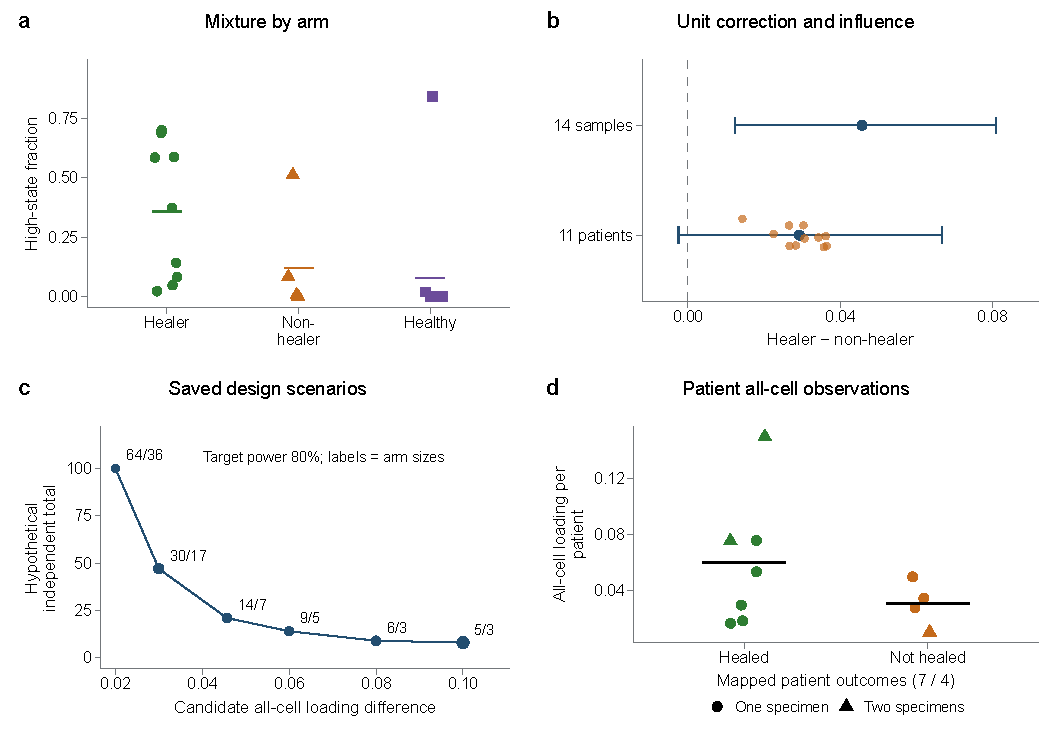
\includegraphics[width=\linewidth]{journal-figures/paper1_figure4_outcome_counterexample.pdf}
\caption{State abundance, analysis unit and saved design scenarios. (a) High-state fractions for 9 healing, 5 non-healing and 11 healthy specimens, with arm means. The healthy maximum 0.841 challenges exclusivity to healing ulcers. (b) All-cell mean-loading effects and bootstrap 95\% intervals for 14 specimens versus 11 patients; orange points retain all 11 patient omissions, not additional outcomes. (c) Six previously calculated all-cell loading-difference scenarios targeting 80\% power; labels show hypothetical healed/non-healed arm sizes. The specimen-derived spreads and independent-observation assumption are not patient-population variance estimates. These scenarios differ from the historical 24.9\% power calculation for a 9-versus-5 high-state-fraction design and are not clinical minimum important differences. (d) All-cell scores of the 7 healed and 4 non-healed patients, with arm means and symbols for one or two contributing specimens. a and d have different cell denominators; none of these displays supplies independent prognostic validation.}\label{fig:p1f4}\end{figure}

\begin{figure}[htbp]\centering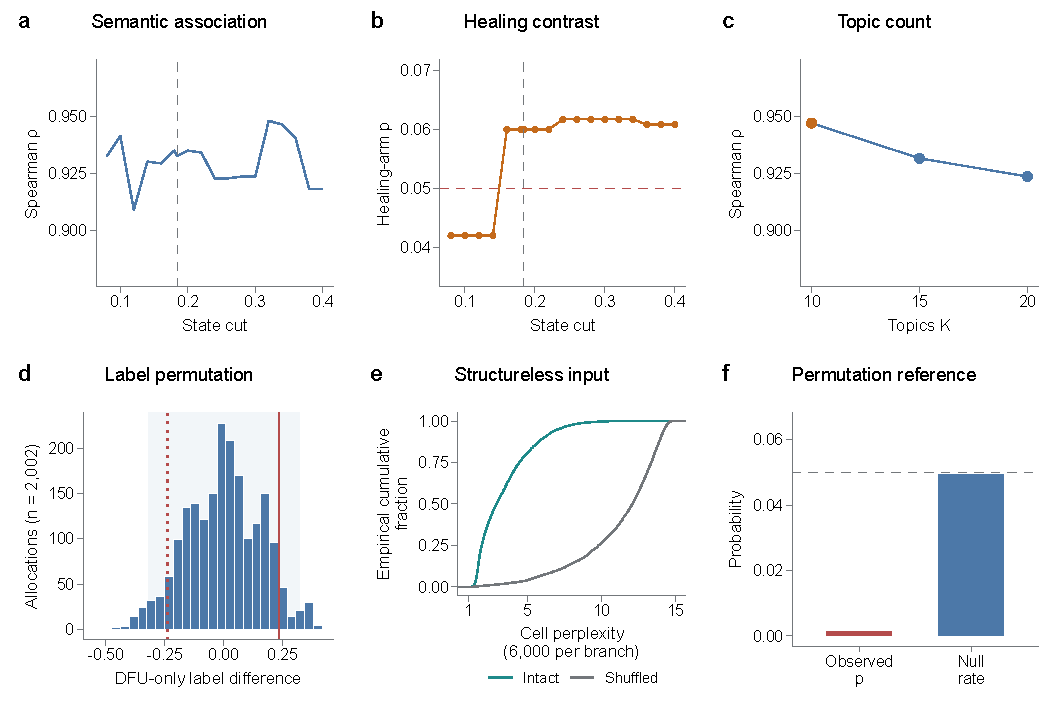
\includegraphics[width=\linewidth]{journal-figures/paper1_figure6_sensitivity_negative_controls.pdf}
\caption{Threshold, capacity and negative-control analyses. (a) Mean--fraction correlation at 18 cuts across 25 specimens; dashed line: pooled cut. (b) Healing-arm Mann--Whitney probabilities for 9 versus 5 specimens; 4/18 are below 0.05. (c) Correlations at K=10, 15 and 20; orange marks K=10, where the healthy-skin maximum fails. (d) The complete saved distribution of 2,002 DFU-only label allocations, with central 95\% shading, positive observed difference and its negative counterpart for the two-sided comparison (p=0.1199). (e) Empirical cumulative perplexity distributions of the 6,000 intact and 6,000 gene-shuffled cells. Their mean perplexities are 3.44 and 11.23 of 15; shuffling also changes row-library variation, so this is not a complete technical null. (f) The separate anatomical specimen-level permutation reference: observed p=0.0015 and 5.0\% of permuted probabilities below 0.05. Cells and label allocations are computational units, not extra patients; repeated specimens limit inference, and no panel establishes pipeline-wide error control.}\label{fig:p1f6}\end{figure}

\begin{figure}[htbp]\centering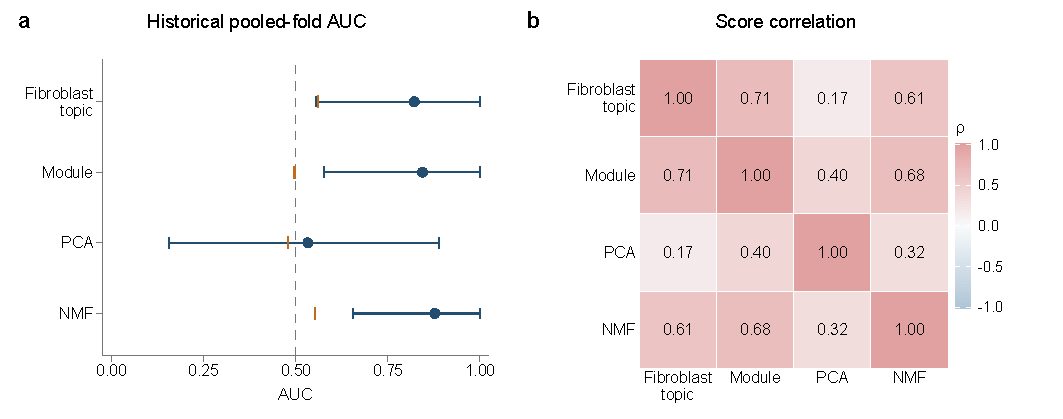
\includegraphics[width=\linewidth]{journal-figures/paper1_figure7_representation_inference.pdf}
\caption{Historical scoring diagnostics in 14 DFU specimens (9 healing, 5 non-healing). (a) Leave-one-sample-out ROC areas (AUCs) with percentile 95\% intervals from 4,000 arm-stratified bootstrap draws of fixed out-of-fold scores, using common resampling indices. Orange ticks: permutation-null means after rerunning outcome-dependent fitting and orientation; dashed line: 0.5, not the fitted null. Fibroblast topic is the frozen all-cell mean; Module is the specified fibro-inflammatory score; PCA and NMF denote principal component and nonnegative matrix readouts. Different fitted-fold coordinates and repeated patients prevent these pooled AUCs or intervals from supporting a representation ranking. (b) Spearman correlations of the same 14 specimen readouts; colours and numbers encode the same statistic. These are procedure diagnostics, not independent patient validation.}\label{fig:p1f7}\end{figure}

\begin{figure}[htbp]\centering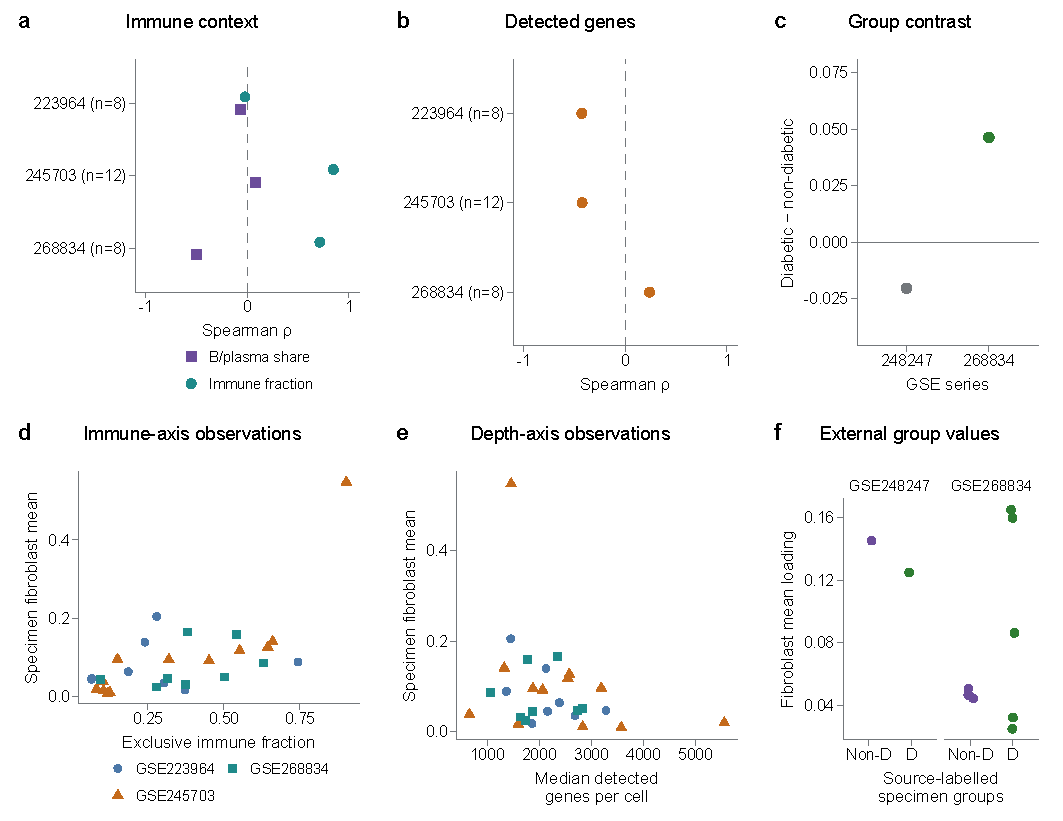
\includegraphics[width=\linewidth]{journal-figures/paper1_figure9_external_construct_audit.pdf}
\caption{External tissue-context projections, not healing validation. (a) Saved correlations with exclusive immune fraction and B/plasma share. (b) Saved correlations with median detected genes per cell. (c) Diabetic-minus-non-diabetic fibroblast contrasts: +0.0464 in GSE268834 and −0.0204 in GSE248247. (d) All specimen fibroblast means against exclusive immune fractions in the three cohorts (8, 12 and 8 specimens). (e) The same observations against median detected genes per cell. (f) Individual source-labelled diabetic and non-diabetic specimen values in the two group comparisons; GSE248247 has only one specimen per group. Correlations and raw points summarize the same data, not separate replications. Gene coverage, tissue sampling and cell yields differ, authoritative healing outcomes are absent, and no biological confidence intervals are inferred.}\label{fig:p1f9}\end{figure}

\begin{figure}[htbp]\centering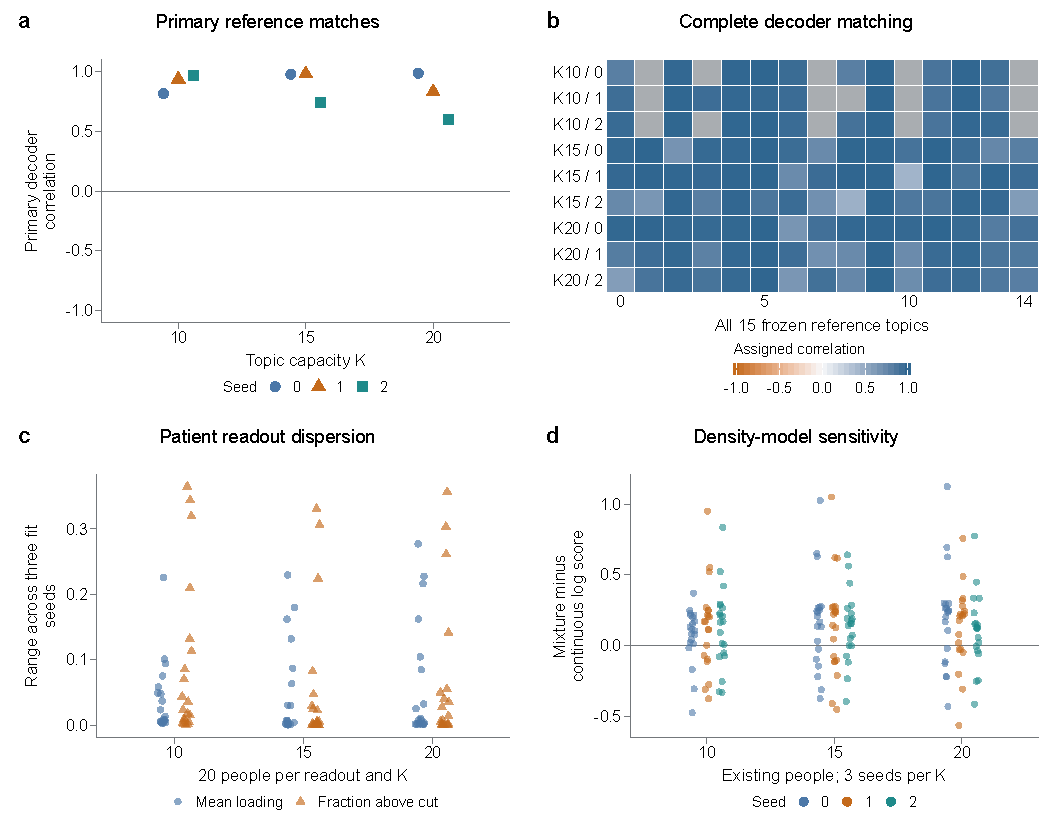
\includegraphics[width=\linewidth]{journal-figures/paper1_figure10_topic_stability.pdf}
\caption{Prespecified capacity and training-seed sensitivities in the original discovery cohort. (a) All nine 40,000-step fits retain their one-to-one assigned match to frozen reference topic 0, without favorable-seed selection. Correlation compares square-root decoder gene probabilities; a missing primary match is unavailable rather than rescued with a rowwise best match. (b) Every reference-topic assignment is shown; gray cells are unmatched or undefined, not low-valued assigned correlations. Capacity K=10 necessarily leaves at least five of the 15 reference topics unmatched. (c) Each point is one existing person's range across three seeds at a fixed K, separately for mean loading and fraction above the fit-specific fibroblast cut. The plotted population is fibroblast-only; complete all-cell counterparts and unavailable counts accompany the tables. Equal-specimen means within patient define this sensitivity experiment, not the primary cell-pooled outcome estimand. (d) Points are person-averaged held-cell log-score differences for a two-component mixture versus a continuous density, on fit-specific transformed topic scores. Positive values favor the mixture under that predictive density comparison. Cell splits and threshold exclusions do not make the full-discovery trained representation independent. Seeds, capacities and points do not add biological patients or validate a discrete state, healing biomarker or amputation endpoint.}\label{fig:p1f10}\end{figure}

\FloatBarrier
\begingroup\setlength{\bibsep}{0pt}

\section*{Supplementary Methods}

\subsection{Prespecified capacity and training-seed sensitivity}
A separate fixed grid uses K=10, 15 and 20, seeds 0--2, 40,000 optimizer steps, batches of 256, learning rate 0.001 and KL weight 0.01 in all nine fits. Every fit uses the existing full-discovery gene panel, cell QC, patient map and lineage labels. Healing labels are not used to choose a capacity, seed, topic match or stopping rule. The training budget is fixed, not a convergence guarantee. The square-root decoder probabilities are matched to the frozen 15-topic decoder by one-to-one Hungarian assignment using Pearson correlation. Primary reference topic 0 remains the reference regardless of assignment quality; unmatched, negative and undefined matches are retained without rowwise rescue. Smaller capacity necessarily leaves reference programmes unmatched. Full inference checkpoints, original cell identities and all topic weights are preserved in one canonical result tree and reprojected on CPU before reporting.

The descriptive midpoint is fitted to all fibroblast loadings within each fit and is not a held-patient or independently validated cut. The new sensitivity summaries average specimens equally within each of the 20 existing people, separately for fibroblast-only and all-cell populations. The same fibroblast-derived cut applied to all cells is an operational loading fraction, not fibroblast-state prevalence. These summaries do not replace the primary cell-pooled patient outcomes. Person-specific min--max ranges across three seeds quantify computational dispersion only. The existing density comparison is also repeated on each fitted score, retaining all five comparisons and unavailable specimens; its shape construction excludes the scored person's specimens, while the expression representation itself remains trained on full discovery expression. Mixture versus continuous held-cell likelihood therefore evaluates conditional score geometry, not independent biological state identity.

The conditional density audit uses logit scores clipped to $[10^{-7},1-10^{-7}]$, a maximum of 4,000 cells per specimen, at least 50 cells and 20 positive scores, and ten random cell half-splits scored in both directions. Reference shapes use only the other patients' specimens, pooled after the per-specimen cap. C1 shifts a shared centered density; C2 shifts and rescales it. M1 reweights two shared components derived from an outcome-blind two-Gaussian responsibility fit; M2 also shifts both components. H1 uses reference components separated at the reference-only cut, with its weight equal to the training-half fraction above that cut. The respective numbers of specimen-level parameters are one, two, one, two and one. Every family shares a Bernoulli zero-mass term when exact zero scores occur. Grid densities have a fixed $10^{-6}$ uniform interior contribution and $10^{-6}$ total exponential-tail mass with scale equal to training-grid width/8. Held-cell log predictive density is averaged equally across split directions and repetitions, then equally across specimens within person. Positive differences favor the first named family in transformed-score nats/cell. The five retained comparisons are M1--C1, M2--C2, M1--C2, H1--C1 and M1--H1; no sign-test probabilities or biological class labels are inferred.
\subsection{Cohort selection and independent units}
GSE165816 comprises 54 original samples and 27 author-mapped participants. The frozen model used 25 selected foot-skin samples in the non-diabetic, DFU-healing and DFU-non-healing groups: 81,602 cells before cell quality control and 76,461 afterwards. Cells required at least 200 detected genes and a mitochondrial count fraction at most 0.20; genes required detection in at least 10 cells before panel selection. The final panel contained 7,002 genes, obtained from a nominal 7,000-gene dispersion selection with retained anchor genes. The discovery outcome subset contained 9 healing and 5 non-healing samples.

The clinical supplement maps those 14 outcome samples to 11 patients: 7 healing and 4 non-healing. G4/G23, G7/G8 and G33/G34 are repeated samples from the same wound on the same day. We combine each patient's retained cells before computing the primary patient score. The outcome is the study's healing category within a 12-week follow-up window, not a measured individual healing time. Amputation events, time to amputation and amputation-risk prediction were not evaluated. Non-healing labels are not treated as amputation events. Series metadata describe a shared Emory 10x Chromium 3$'$ V2/V3 workflow and NovaSeq instrumentation; the absence of per-sample chemistry and flow-cell identifiers prevents run-specific batch adjustment.

\subsection{What the frozen neural topic model computes}
For nonnegative panel counts $x_{ig}$ with positive total, let $u_{ig}=x_{ig}/\sum_{h=1}^{G}x_{ih}$. The implemented model uses a diagonal-Gaussian encoder in unconstrained coordinates and a softmax decoder:
\begin{align}
q_\phi(z\mid u_i)&=\mathcal N\!\left(\mu_\phi(u_i),\operatorname{diag}\sigma_\phi^2(u_i)\right),\label{eq:p1encoder}\\
\theta_{ik}&=\frac{e^{z_{ik}}}{\sum_{\ell=0}^{K-1}e^{z_{i\ell}}},\qquad
\beta_{kg}=\frac{e^{b_{kg}}}{\sum_{h=1}^{G}e^{b_{kh}}},\qquad
\widehat u_{ig}=\sum_{k=0}^{K-1}\theta_{ik}\beta_{kg}.\label{eq:p1decoder}
\end{align}
Equations~\eqref{eq:p1encoder}--\eqref{eq:p1decoder} define the encoder, simplex coordinates and normalized topic-gene decoder used below. Thus $\theta_i\in\Delta^{K-1}=\{a\in\R^K:a_k\geq0,\sum_{k=0}^{K-1}a_k=1\}$ and every topic-gene row sums to one. The topic indices start at zero. A Gaussian mapped through softmax gives a logistic-normal representation. This differs from a Dirichlet prior, while retaining the mixture representation that motivates topic models. Training minimizes
\begin{equation}
\mathcal L(\phi,b)=\frac1N\sum_i\E_{q_\phi}\!\left[-\sum_g u_{ig}\log(\widehat u_{ig}+10^{-10})\right]
+0.01\,\frac1N\sum_i\operatorname{KL}\!\left(q_\phi(z\mid u_i)\,\|\,\mathcal N(0,I)\right).\label{eq:p1loss}
\end{equation}
Equation~\eqref{eq:p1loss} is the fitted objective: each cell contributes cross-entropy on its panel proportions, followed by a Gaussian regularizer. It is neither a depth-weighted count likelihood nor an unmodified evidence lower bound for such a likelihood. With encoder log-variance $\ell_{ik}=\log\sigma_{ik}^2$, the reparameterization and regularizer are
\begin{equation}
z_{ik}=\mu_{ik}+e^{\ell_{ik}/2}\epsilon_{ik},\quad \epsilon_i\sim\mathcal N(0,I),\qquad
\operatorname{KL}_i=\frac12\sum_k\left(\mu_{ik}^2+e^{\ell_{ik}}-1-\ell_{ik}\right).\label{eq:p1gaussian}
\end{equation}
Equation~\eqref{eq:p1gaussian} is the diagonal-Gaussian calculation used by the implementation; one noise draw per cell estimates the reconstruction expectation in each training batch. The encoder has widths 256 and 128, batch normalization, ReLU activations and dropout 0.1. The recorded fit used $K=15$, 40,000 Adam steps, learning rate $10^{-3}$ and batches of 512. Deterministic projection disables encoder dropout and uses $z=\mu_\phi(u)$ and $\theta=\operatorname{softmax}(\mu_\phi(u))$, which is not generally $\E_q[\operatorname{softmax}(z)]$. Missing panel genes in external projections are set to zero. Normalization and quality control can alter biological interpretations, so this definition is kept distinct from other variance-stabilizing methods.

Topic-gene perplexity is summarized as $\exp\{-K^{-1}\sum_{k,g}\beta_{kg}\log\beta_{kg}\}$; it measures concentration of decoder weights, not superiority over other representations. The latent coordinate $\mu\in\R^K$ is not the simplex coordinate $\theta$. Softmax is unchanged by adding a common scalar to all coordinates of a cell; reconstruction therefore does not identify that offset. The Gaussian penalty constrains the fitted coordinates but does not give them a unique biological interpretation. Topic weights are decoder coefficients, not independently calibrated probabilities of membership in a biological cell type.

\subsection{Separate budget and training-panel diagnostics}
Six previously completed diagnostic fits examine optimization budget and panel selection without replacing the frozen discovery measurement. An outcome-blind patient-identity split assigns 16 patients (60,861 cells) to optimization and four patients (15,600 cells) to evaluation across all clinical groups. Each fit uses $K=15$, batch size 128, Adam learning rate $10^{-3}$ and KL weight 0.01. Two seeds are fitted from initialization at 20,000 and 40,000 steps on the inherited 7,002-gene panel; two further 20,000-step fits use a 7,003-gene panel selected by support and dispersion only in training patients, retaining the prespecified anchor genes. The upstream gene universe, cell QC and lineage labels remain discovery-derived. This is not end-to-end independent or DFU-only clinical validation.

Fixed 128-cell evaluation draws per patient are scored with equal patient weight. Held reconstruction, excluding KL, is compared only with its own panel's training-cell mean and equal-training-patient mean nulls. Different panels change the probability space and normalization denominator, so their raw cross-entropies are not ranked. Decoder separation uses cosine between square-root topic-gene rows; effective usage is the exponential entropy of mean held topic weights. The engineering plateau screen requires each of the last five absolute 100-step objective movements to be at most 0.001, separately for training and held patients. It is neither a stopping rule nor proof of mathematical convergence. Reference-topic matching uses a discovery-trained decoder that includes held expression and is not used to select a seed or panel. The historical diagnostic patient readouts equally weight specimens, unlike the cell-pooled primary measurement. All six fits and failed screens are reported (Supplementary Table~S33).

A saved-evidence pooling bridge reaggregates the existing deterministic coordinates for all six fits without a new model fit, encoder call, checkpoint reload or threshold fit. Within each patient, the fibroblast mean and high-score fraction pool recovered fibroblasts across specimens; the comparison equally weights specimen fibroblast summaries. The high rule is strictly above each fit's saved training-only cut. The saved one-to-one topic assignment and cut are retained, not selected or harmonized across fits. Report artifacts, source manifests and completion records are checked against SHA-256 bindings, including each fit's receipt-bound topic/cut contract. All 120 patient--fit rows reuse the same 20 patients; training and held summaries retain the fixed 16/4 partition. These are weighting comparisons conditional on each diagnostic representation, not replacements for the primary frozen discovery values or independent healing tests (Supplementary Table~S36, S37 and~S38).

Complete saved patient-fit pooling comparisons are provided in Supplementary Table~S38.

\subsection{Threshold fractions and the exact mean decomposition}
Let $Y_{si}=\theta_{si,\star}$ for fibroblast-gated cell $i$ in sample $s$. The discovery lineage gate averages marker expression standardized across the selected discovery cells, then assigns the highest-scoring lineage. Its markers are disjoint from the tested topic-gene list by an explicit overlap check. The gate remains an expression-based operational definition; its reference population can change its assignments, and the frozen encoder alone does not freeze the complete tissue measurement. A pooled two-Gaussian fit provides a descriptive cut $c=0.1842958$, the midpoint of the fitted component means. Gaussian components approximate a bounded score distribution and are not assumed to be literal biological populations.
\begin{equation}
\bar Y_s=\frac1{n_s}\sum_iY_{si},\qquad
\widehat w_s(c)=\frac1{n_s}\sum_i\ind\{Y_{si}>c\}.\label{eq:p1fraction}
\end{equation}
Equation~\eqref{eq:p1fraction} defines both the sample mean and the reported hard-threshold fraction; the latter is not an average posterior responsibility of the Gaussian mixture. Define $\bar Y_{s,L}$ and $\bar Y_{s,H}$ as means below/at and above the cut. Then, with empty-component contributions interpreted as zero,
\begin{equation}
\bar Y_s=(1-\widehat w_s)\bar Y_{s,L}+\widehat w_s\bar Y_{s,H}.\label{eq:p1identity}
\end{equation}
Equation~\eqref{eq:p1identity} is exact. Only under an additional approximate component-stability assumption, $\bar Y_{s,L}\approx m_L$ and $\bar Y_{s,H}\approx m_H$, does it reduce to $\bar Y_s\approx m_L+(m_H-m_L)\widehat w_s$. Consequently, a large correlation between the two summaries cannot independently prove stable intensity: both summaries use the same cells. Persistence of overlapping low-state tails supplies complementary distributional evidence. The 10th percentile of a high-loading sample (0.029) overlaps the scale of the 90th percentile in a low-loading sample (0.119); this observation alone is not a formal test of multimodality.

To quantify the term omitted by a constant-state approximation, let $m_L,m_H$ be the cell-pooled means in the two threshold bins across the 19,410 discovery fibroblasts. They are empirical bin means, not the fitted Gaussian means. For each specimen,
\begin{align}
A_s&=(1-\widehat w_s)m_L+\widehat w_sm_H,\notag\\
R_s&=(1-\widehat w_s)(\bar Y_{s,L}-m_L)+\widehat w_s(\bar Y_{s,H}-m_H),\qquad \bar Y_s=A_s+R_s.\label{eq:p1residual}
\end{align}
Equation~\eqref{eq:p1residual} separates a specified constant-state approximation from its exact residual. An empty bin contributes zero and its undefined mean is omitted from the corresponding mean range. We summarize all 25 specimens using specimen-weighted residual RMS and bin-mean ranges. These are finite-data descriptions without a test of state invariance or a causal allocation of variance (Supplementary Table~S19).

The semantic statistic is $\rho_{\rm sem}=\operatorname{cor}_{\rm Spearman}(\bar Y_s,\widehat w_s)$ across 25 samples. A 10,000-draw sample-row percentile bootstrap, 10,000 row permutations and leave-one-sample-out recalculation characterize its stability. These do not create independent patients. The patient-collapsed correlation of 0.937 across 20 mapped patients and its descriptive patient-resampling interval are the primary uncertainty summary; the earlier specimen resampling is historical.

A separate patient-resampling analysis collapses the 25 specimen means and high-state fractions to 20 patients using fibroblast counts as within-patient weights. It draws 10,000 patient samples with replacement (seed 217) and reports the percentile interval for their Spearman correlation. Leave-one-patient-out analyses recompute this correlation across the remaining 19 patients and separately recompute the all-cell healing contrast across the remaining 10 outcome patients. The reported omission range is a sensitivity diagnostic, not an interval estimate (Supplementary Table~S16).

\subsection{Technical controls and constant sensitivity}
Dissociation-induced programmes and ambient transcripts motivate the technical controls. The stress comparison uses a standardized mean difference (SMD) with rejection bound 0.8; the doublet-oriented control compares PTPRC-positive rates with ratio bound 2.0. Exact panel-count matching reprojects downsampled counts, comparing cell labels and sample fractions. The historical 31-covariate screen retains its specimen-row asymptotic p values and BH transforms for auditability, not as valid patient-level significance or false-discovery-rate control: repeated patients violate the naive independent-row premise. Removing any cell carrying a specified immune transcript tests invariance to that exclusion rule. This cannot by itself identify ambient contamination or exclude every doublet. Residual mixture checks with immune covariates are compared with four unrelated placebo covariates; similarly flattened residuals limit claims of statistical separability.

Sensitivity fits use 18 cuts between 0.08 and 0.40 (including the rounded fitted cut) and $K\in\{10,15,20\}$. The TIMP1-carrying topic is tracked descriptively across capacities; topic labels are not assumed exchangeable or biologically identical across $K$. The anatomical positive-control calibration uses 20,000 shuffles. The raw-count structure control selects a fixed 6,000-cell subset by the recorded source order, then permutes each gene's observed values across cells with a seeded permutation; this preserves the marginal multiset for each gene but does not preserve row-wise library sizes. The resulting topic concentration, row-wise library-size and detection-rate summaries are compared with real input; no new topology audit is performed. The separate outcome-label calibration exhaustively enumerates all 2,002 allocations of the 9 healing and 5 non-healing specimens, retaining repeated specimens as a specimen-unit null. It is not a patient-level clinical test or proof of pipeline-wide error control. The DFU-only label null excludes all healthy controls before allocation and reports the 9/5 specimen result as secondary to the 7/4 patient test. For each specimen, a continuous-score construction applies the inverse-logit transform to its observed mean on the logit scale plus independent standard-normal noise, retaining its cell count; 200 seeded draws are made without a latent class or mixture fit. The constructed mean need not equal the observed mean. This is an illustrative non-identification example, not a fitted null model or a calibrated probability. These analyses are retrospective computational controls, not a registered clinical trial.

For marker-reference sensitivity, expression is normalized per cell to 10,000 counts and transformed by log1p. Each lineage score averages its marker-wise standardized values, followed by exclusive maximum-score assignment. The pooled marker means and SDs are frozen before applying the same reference to each specimen; this implementation check is compared with re-estimating means and SDs separately within each specimen. The topic encoder and state threshold remain fixed. Patient contrasts are recomputed after count-weighted pooling under each annotation reference, with the three readouts forming a separate BH family within each gate. This evaluates dependence on the annotation reference without an independent cell-identity truth set (Supplementary Table~S26).

The exploratory covariate scan retains the original rounded rule $Y_{si}\geq0.184$, used by the technical-control analyses, rather than substituting the fitted cut 0.1842958. It correlates the sample high-state fraction with 14 other fibroblast topic means, 11 whole-sample lineage fractions, total and fibroblast cell counts, fibroblast dissociation score, median UMI count, PTPRC-positive fraction and the numeric G specimen label. Two-sided Spearman probabilities are adjusted across all 31 comparisons by Benjamini--Hochberg. The 25 rows are specimens, include repeated patients, and receive no clinical-outcome adjustment. The G label is an identifier covariate, not a verified sequencing batch or collection time. Topic coordinates and lineage fractions have compositional dependence.

The patient-level descriptive update retains the same 31-covariate family without selecting significant rows. It uses the current deterministic coordinates and fitted midpoint: fibroblast topic means and high fractions pool recovered fibroblasts within patient, whereas lineage fractions pool lineage counts and divide by all patient cells. Cell-count covariates sum across specimens. Dissociation, PTPRC positivity and median-UMI summaries are fibroblast-count-weighted averages of their saved specimen values; the UMI summary is not a pooled-patient median. The G-number summary averages specimen labels equally within patient. Spearman correlations and all 20 leave-one-patient-out recalculations are descriptive. This unblinded scan supplies no p values, BH discoveries, adjusted associations or new biological replication (Supplementary Table~S32).

The saved DFU-only extension restricts that same family and unchanged high-fraction target to the 11 author-mapped DFU patients (14 specimens; seven healed, four non-healed), excluding nine non-diabetic patients. Healing labels define the subset but are not the correlation endpoint. It preserves the existing patient aggregation and cut 0.184295848, reports every pairwise-finite denominator and retains all 31 full correlations and 341 single-patient omissions. The mixed-20 comparator and its omission summaries were reproduced against the producing report before restriction; report/source/completion SHA-256 bindings are verified before export. Omission extrema and sign changes describe influence, not confidence intervals. Removing the non-diabetic arm does not remove within-DFU technical, compositional or clinical confounding. No p values, BH discoveries, outcome regression, causal interpretation, new fit or resampling is added (Supplementary Table~S34 and~S35).

Complete omission-level correlations are provided in Supplementary Table~S35.

\subsection{Full released-count depth sensitivity}
The full-pipeline stress test starts from all 81,602 released count columns in the 25 selected specimens, including cells failing the original analysis QC. These are processed count matrices, not pre-cell-calling droplets or sequencing reads. Baseline reconstruction must reproduce retained cell identities, lineage assignments and deterministic coordinates before perturbation. Each nonzero count is independently thinned with a binomial probability of 0.75, 0.50, 0.25 or 0.10, with three fixed computational seeds per rate. Every rate starts from the original counts; no cells or patients are resampled. QC is rerun using at least 200 detected genes and a mitochondrial fraction at most 0.20. The discovery marker reference, exclusive maximum-score gate, panel, encoder and high-state threshold remain unchanged; there is no new margin or outcome-guided label rule.

The full-pipeline population includes all current QC survivors and uses newly computed labels. Separate conditional branches retain original QC cells and labels, retain the QC intersection with original labels, or re-gate the same intersection. Lost and newly admitted cells, lineage transitions and fibroblast entry/exit are reported separately. Zero detected annotation markers and tied winning scores are diagnostics, not evidence of valid cell identity. A zero panel total makes a score missing, rather than assigning the encoder output of a zero vector. Readouts preserve their selected-cell denominators and are non-estimable if required scores are missing. Patient aggregation pools the appropriate all-cell or fibroblast counts across repeated specimens. The same seven healed and four non-healed patients supply 330 exhaustive label allocations; the three seed ranges describe perturbation sensitivity, not biological confidence intervals or new outcome tests. Uniform thinning does not model upstream cell calling, cell-type-specific capture, ambient RNA, doublets or independent tissue sampling.

\subsection{Patient contrast, permutation and equivalence sensitivity}
Let $\mathcal C_p$ contain all retained cells in the mapped DFU foot specimens of patient $p$. The separate all-cell score is $S_p=|\mathcal C_p|^{-1}\sum_{i\in\mathcal C_p}\theta_{i\star}$, so repeated specimens contribute in proportion to retained cell counts. This all-cell readout differs from $\bar Y_s$ restricted to fibroblasts and from $\widehat w_s$. For healing set $H$ and non-healing set $N$,
\begin{equation}
\widehat\Delta=\frac1{|H|}\sum_{p\in H}S_p-\frac1{|N|}\sum_{p\in N}S_p.\label{eq:p1delta}
\end{equation}
Equation~\eqref{eq:p1delta} defines the all-cell patient contrast, separate from the fibroblast-restricted readouts. All $\binom{11}{7}=330$ patient-label allocations are enumerated, including the observed assignment and ties:
\begin{equation}
p_{\rm exact}=\frac{\sum_{\pi\in\Pi}\ind\{|\widehat\Delta_\pi|\geq|\widehat\Delta|\}}{|\Pi|}.\label{eq:p1permutation}
\end{equation}
Equation~\eqref{eq:p1permutation} is the exhaustive two-sided probability reported here. Archived legacy calculations used an add-one convention, but that extra correction is unnecessary for exhaustive enumeration and is not a second inferential result in this article. Exchangeability remains an assumption for observational labels. A 30,000-draw bootstrap resamples patients within outcome arms; bootstrap intervals and permutation tests need not be dual.

The saved exhaustive enumeration gives the numerical all-cell comparison:
\begin{equation}
p_{\rm exact}=\frac{\#\{\pi\in\Pi:|\widehat\Delta_\pi|\geq|\widehat\Delta|\}}{|\Pi|}=\frac{90}{330}=0.272727.\label{eq:p1exact}
\end{equation}
Equation~\eqref{eq:p1exact} includes the observed allocation and numerical ties. It distinguishes exhaustive enumeration from randomly sampled permutations; the primary comparison uses exhaustive enumeration without an add-one correction. Neither convention makes observational healing labels randomized or tests a causal effect. Supplementary Table~S20 reports the independent arithmetic check, including the Welch quantities below.

For a symmetric equivalence margin $M$, the Welch two-one-sided-test procedure uses $SE=(s_H^2/n_H+s_N^2/n_N)^{1/2}$ and Welch degrees of freedom $\nu$:
\begin{equation}
p_L=1-F_{t_\nu}\!\left(\frac{\widehat\Delta+M}{SE}\right),\qquad
p_U=F_{t_\nu}\!\left(\frac{\widehat\Delta-M}{SE}\right).\label{eq:p1tost}
\end{equation}
Equation~\eqref{eq:p1tost} gives the two one-sided tests used for a prespecified margin. Both must be below 0.05 to reject non-equivalence. Writing $v_H=s_H^2/n_H$ and $v_N=s_N^2/n_N$ makes the degrees of freedom and margin boundary explicit:
\begin{equation}
\nu=\frac{(v_H+v_N)^2}{v_H^2/(n_H-1)+v_N^2/(n_N-1)},\qquad
M_*=|\widehat\Delta|+t_{\nu,0.95}SE.\label{eq:p1margin}
\end{equation}
Equation~\eqref{eq:p1margin} is the infimum margin containing the two-sided 90\% Welch interval; strict rejection requires $M>M_*$. Independent calculation gives $SE=0.019446$, $\nu=8.113833$ and $M_*=0.065375$ for the 11-patient comparison. The deterministic specimen-unit boundary is 0.079644. A margin selected after seeing these data is a sensitivity summary, not a clinically justified equivalence claim. No clinical minimum important difference has been supplied.

\subsection{Discrimination, anatomy and design simulations}
For held-out prediction scores $r$, AUC is the empirical probability that a healing score exceeds a non-healing score, with half credit for ties:
\begin{equation}
\widehat{\rm AUC}=\frac1{n_Hn_N}\sum_{h\in H,n\in N}\left[\ind\{r_h>r_n\}+\tfrac12\ind\{r_h=r_n\}\right].\label{eq:p1auc}
\end{equation}
Equation~\eqref{eq:p1auc} is the pairwise empirical AUC used for the held-out scores. Topic orientation, module preprocessing and the choice of PCA/NMF components are determined inside each training fold. The topic encoder itself was trained without outcomes on the discovery cohort, including held-out patients' expression: this is an internal discrimination audit of a frozen discovery representation, not fully external representation validation. Bootstrap intervals resample fixed out-of-fold scores with common arm-stratified indices across methods; the entire fitting/orientation process is rerun for label permutations. All allocations are used for topic and module readouts; PCA and NMF use 200 sampled relabellings. Sample-level comparisons use 14 specimens and patient-level comparisons use 11 mapped patients; they are not interchangeable.

PCA scaling and basis fitting, and NMF fitting, use training rows only. The historical pooled out-of-fold AUC nevertheless compares scores from different fitted folds; those scores are not calibrated clinical risks. Separate PCA and NMF fits can change the selected coordinate, origin and scale between folds. AUC is invariant to a common increasing transformation, but not to separate fold-specific transformations. These raw-coordinate AUCs and their fixed-score bootstrap contrasts are retained as historical scoring diagnostics, not evidence for a representation ranking.

The revised patient discrimination audit instead leaves out one healing patient $h$ and one non-healing patient $n$ together. Each of the $7\times4=28$ folds fits one scoring function $r^{(-h,-n)}$ to the remaining nine patients (six healing, three non-healing), and that unchanged function scores both excluded patients:
\begin{equation}
\widehat A_{\rm pair}=\frac1{28}\sum_{h\in H,n\in N}\left[\ind\{r^{(-h,-n)}_h>r^{(-h,-n)}_n\}+\tfrac12\ind\{r^{(-h,-n)}_h=r^{(-h,-n)}_n\}\right].\label{eq:p1pairauc}
\end{equation}
Equation~\eqref{eq:p1pairauc} averages within-model pair orderings; no raw scores from different fitted models are compared. Patient expression inputs are cell-count-weighted means of per-cell proportions on the fixed panel. Topic orientation, module gene standardization and orientation, PCA standardization and fitting, and NMF fitting and component selection use training patients only. The PCA rule selects the largest absolute training-arm mean difference among five components. NMF uses five components and tolerance $10^{-4}$; the initial 1,000-iteration cap was raised uniformly to 10,000 after three training fits reached the cap, without using held-pair discrimination to select it. The initial run is retained, and no final fit emitted a convergence warning. Fitted basis rows are normalized to unit Euclidean norm before independent nonnegative-least-squares projection of each row. The component is selected by the absolute training-arm mean difference divided by the training-patient SD, making selection invariant to positive component rescaling. The direction is set by the training contrast, and exact ties receive half credit. The fixed gene panel, topic representation and study-specific analysis choices remain discovery-derived. The 28 pairs share 11 patients and overlapping training sets, so they are not 28 independent outcomes; no pair-binomial uncertainty, fixed-score bootstrap interval or significance probability is supplied for this revised estimand. Changing component normalization and selection as well as fold structure means the difference from the historical AUC cannot identify the contribution of one correction alone. Reusing the same cohort to inspect readouts limits confirmatory interpretation.

The paired anatomical control tests foot-minus-forearm differences in 10 mapped patients using all $2^{10}$ sign allocations and the same add-one convention. Across 15 topics, Benjamini--Hochberg adjustment is $q_{(i)}=\min\{1,\min_{j\geq i}15p_{(j)}/j\}$, with the usual assumptions required for false-discovery-rate interpretation.

The historical high-state-fraction power calculation uses 9 versus 5 specimens, Gaussian location shifts with pooled SD 0.283 and a two-sided Mann--Whitney test. Its 24.9\% power and $\operatorname{MDE}_{0.8}=0.519$ apply to this approximate design, not to the 11-patient all-cell contrast. Gaussian simulation can leave the unit interval, so it is a design-scale sensitivity approximation. A separate next-cohort simulation uses specimen-derived arm SDs of deterministic all-cell mean scores, 0.05170 and 0.01686, Welch testing or Welch equivalence testing, and 4,000 draws per candidate size. These descriptive spreads include repeated specimens and are not independent-patient variance estimates. The candidate totals are approximate conditional calculations, not validated recruitment targets (Supplementary Table~S6).

\subsection{External projections and limits of identification}
Every external cohort is projected into the frozen panel/model without outcome-guided retuning. The immune and B/plasma gates exclude promiscuous markers such as CD74, CD37, CD38 and SDC1 and assign non-overlapping compartments. Immune fraction uses all retained cells as its denominator; B/plasma share within immune cells uses only that compartment. Their correlations estimate different quantities. Negative depth correlations cannot by themselves exclude depth confounding, because a marginal sign is not a conditional adjustment.

GSE231643 supplies eight title-labelled specimens but lacks an authoritative patient mapping. GSE241132 contributes an acute-wound, three-donor construct summary. GSE223964, GSE245703 and GSE268834 lack qualifying patient-level healing endpoints, and GSE248247 has only two samples. We do not pool these correlations or describe them as independent prognostic validation. No analysis identifies a treatment effect, a time-to-healing model or a causal effect of immune infiltration.

\subsection{Observed-cell and expression displays}
The biological displays reuse the saved 15-topic cell proportions and operational lineage assignments. For visualization only, each proportion vector is transformed to centered log ratios,
\begin{equation}
c_{ik}=\log\theta_{ik}-K^{-1}\sum_{\ell=0}^{K-1}\log\theta_{i\ell}.\label{eq:p1display}
\end{equation}
Equation~\eqref{eq:p1display} removes the geometric mean of the positive coordinates before a Euclidean-distance UMAP with 30 neighbors, minimum distance 0.3 and random seed 17. All 76,461 cells enter the embedding; a uniform subset of 2,000 cells is drawn for the printed vector panels, using the same cells and coordinates for lineage and loading colors. The sampling affects only display. Neither embedding separation nor displayed point density enters the outcome tests, gate, threshold or model fitting. Two-dimensional maps can distort relationships in the input space and do not establish cell types or trajectories.

Raw discovery matrices are reloaded under the original tissue, disease and cell-quality criteria. We require the retained sample and arm order and all recomputed marker-based labels to match the saved cell table. For each displayed gene, dot size is the fraction of cells with a positive count; color is the mean of cellwise $\log(1+10^4 x_{ig}/\sum_h x_{ih})$, scaled from its smallest to largest lineage mean. The denominator uses the source gene matrix, not only the frozen modeling panel. The 18-gene display includes compartment markers and programme-associated genes without an outcome-based selection step. It illustrates measured expression and cannot independently validate labels derived from some of the same markers. Specimen composition retains each specimen as a separate column, and loading histograms use all assigned fibroblasts in fixed bins of width 0.02.

\subsection{Patient-unit extension of the lineage readouts}
The retrospective extension fixes three readouts before computing their new outcome comparisons: within-fibroblast mean loading, the fraction above the existing mixture midpoint, and fibroblast composition among all retained cells. Let $\mathcal S_p$ denote patient $p$'s specimens, $n_s^F$ their fibroblast counts and $n_s^A$ their all-cell counts. With specimen means $m_s$, threshold fractions $w_s$ and composition fractions $f_s=n_s^F/n_s^A$, the pooled patient summaries are
\begin{equation}
M_p=\frac{\sum_{s\in\mathcal S_p}n_s^F m_s}{\sum_{s\in\mathcal S_p}n_s^F},\quad
W_p=\frac{\sum_{s\in\mathcal S_p}n_s^F w_s}{\sum_{s\in\mathcal S_p}n_s^F},\quad
F_p=\frac{\sum_{s\in\mathcal S_p}n_s^A f_s}{\sum_{s\in\mathcal S_p}n_s^A}.\label{eq:p1lineagepatients}
\end{equation}
Equation~\eqref{eq:p1lineagepatients} pools the appropriate denominators within patient while giving each of the 11 outcome patients equal weight in the group contrast. The representation, annotations and loading cut are unchanged. We enumerate all 330 allocations of seven healed labels among 11 patient rows, counting absolute contrast ties within a numerical tolerance of $10^{-12}$. For this new exhaustive enumeration the probability is the exceeding count divided by 330, without the add-one convention retained in the historical all-cell analysis. The three new probabilities form one Benjamini--Hochberg family. Observational group exchangeability is an assumption, not random assignment of healing outcomes.

Percentile intervals use 10,000 patient resamples separately within the seven healed and four non-healed groups, with seed 17. They are small-sample descriptive intervals, not externally calibrated prediction intervals. Sensitivities replace within-patient count weights by equal specimen weights, omit each patient in turn, and require every retained specimen to have at least 100 fibroblasts. Common random draws are used when the patient arrays coincide. We report when an eligibility sensitivity removes no specimen. The 20-patient descriptive table includes non-diabetic participants, but only the 11 DFU patients enter healing contrasts; no healthy participant is assigned a healing outcome.

\subsection{Patient distributions, cell yield and repeated sampling}
To assess the loading distribution without selecting one state threshold, let $F_p(c)$ be the empirical cumulative distribution of all recovered fibroblast loadings pooled within patient $p$. Each patient contributes a normalized distribution regardless of cell yield. We compare the two equally weighted patient-group distributions using
\begin{equation}
T=\sup_{c\in\mathcal C}\left|\frac1{7}\sum_{p:H_p=1}F_p(c)-\frac1{4}\sum_{p:H_p=0}F_p(c)\right|,\label{eq:p1ecdf}
\end{equation}
where $\mathcal C$ contains every distinct observed loading. Equation~\eqref{eq:p1ecdf} uses the same 11 patients and frozen scores. Its exact probability enumerates all 330 patient-label allocations; this is a patient-level permutation statistic, not a cell-level Kolmogorov--Smirnov test. We also report high-fraction contrasts at cuts 0.05, 0.10, 0.15, 0.20, 0.30, 0.40, 0.50 and 0.60, together with the original midpoint. Comparing each absolute contrast with the permutation distribution of $T$ gives a max-statistic probability across the complete loading support. These retrospective sensitivities and their unadjusted probabilities are shown in Supplementary Table~S23.

Cell-yield sensitivity uses 250 draws of exactly 100 fibroblasts without replacement from each of the 14 DFU specimens, with random seed 29. Each draw averages specimen means and high-state fractions equally within patient before recomputing the 7-versus-4 contrast and exact probability. This changes the contribution of recovered cells, without changing clinical labels or the frozen threshold. Fibroblast composition is not recomputed from this deliberately selected cell subset. Separately, three patients have two specimens each; all $2^3=8$ choices of one specimen per patient are evaluated for all three original readouts. Supplementary Table~S24 gives complete contrast and probability ranges. The draws and specimen choices assess finite-cell and sampling sensitivity, not new patients or confidence bounds.


Repeated-specimen diagnostics retain all five mapped pairs, including three DFU pairs. For each pair we compare fibroblast means, high-state fractions and the supremum difference between empirical loading distributions. Within each specimen, 250 seeded random partitions create disjoint fibroblast halves without replacement; their absolute mean differences provide a conditional cell-sampling reference. We compare each observed between-specimen difference with both within-specimen 97.5th percentiles. These partitions are not biological replicates, patient confidence intervals or an intraclass correlation estimate (Supplementary Table~S28).

\subsection{Selection-aware inference and tissue-context projection}
To examine sensitivity to topic searching, each of the 330 allocations of 7 healed among the 11 DFU patients was scored by the largest healed/non-healed ratio of patient means over all 15 topics. The maximum-calibrated $p$ for named topic 0 is the fraction of allocations whose largest ratio is at least its observed ratio. A global maximum test instead compares with the largest observed ratio, which can belong to a different topic. These patient-weighted statistics are distinct from the original cell-weighted arm selection, and do not reproduce every discovery decision. Topic-specific fraction cuts are fixed from discovery expression before label permutation; they are not independent state definitions. In a separate loop the topic was chosen on ten patients and scored on the held-out eleventh, while the encoder and upstream gene panel remained discovery-trained. The eight intact foot-skin specimens from diabetic donors and all eleven forearm specimens were projected through the frozen QC, gate and model; reprocessing the archive reproduced the primary cells, fibroblasts and labels exactly. Group contrasts use exact permutation of patient means and exact rank tests; presence of high-scoring fibroblasts is a fraction above 0.02. Variance shares follow the exact mean decomposition: with prevalence $w_s$, low- and high-bin means $L_s$ and $H_s$ and their pooled values $\bar L$ and $\bar H$, the fibroblast mean is $A_s+R_s$ with $A_s=(1-w_s)\bar L+w_s\bar H$, and the shares are $\operatorname{Var}(A)$, $\operatorname{Var}(R)$ and $2\operatorname{Cov}(A,R)$ over $\operatorname{Var}(A+R)$. Refit contrasts use each fit's assigned topic and its own cut.


OpenAI Codex (OpenAI) assisted with code development, execution and checking of computational analyses, suggestions for analytical and methodological checks, manuscript drafting and restructuring, extensive language editing, and LaTeX and figure preparation. Reported numerical results were checked against saved outputs, and scripts and document builds were verified using the procedures described in this article and its Supplementary Information. AI-assisted critique and verification are preparation aids and do not constitute independent human peer review. The author directed the work and retains responsibility for the study design, data provenance, choice of analyses, scientific interpretation and final manuscript. No generative images were used as research data.

\bibliographystyle{naturemag}
\bibliography{references_paper1}
\endgroup
\end{document}
